\chapter{Automating Observations of Transient Events}
\label{chap:events}
\chaptoc{}

% ########################################

\newpage
\section{Introduction}
\label{sec:events_intro}
\begin{colsection}

% ~~~~~~~~~~~~~~~~~~~~

\begin{colsection}

In this chapter I outline my work on the systems that allow GOTO to automatically follow up alerts of transient events, specifically gravitational wave detections and gamma-ray bursts. \aref{sec:gototile} describes the \software{Python} module GOTO-tile, which is used to create the all-sky grid that probability skymaps are mapped onto. The module was originally created by Darren White and then expanded by Evert Rol before I took over development, and the functions to create Gaussian skymaps were originally written by Yik Lun Mong. \aref{sec:gotoalert} describes another \software{Python} module GOTO-alert, which contains the structures and functions to process alerts published by LIGO, NASA and other sources. This module was originally based on work by Alex Obradovic before I took over the code and developed it to work with the other GOTO modules. All work described in this chapter is my own and has not been published before anywhere else.

\end{colsection}

% ~~~~~~~~~~~~~~~~~~~~

\subsection{Transient astronomy}
\label{sec:transient_astronomy}
\begin{colsection}

For the last few decades the number of detections of transient astronomical sources has been rapidly increasing. From space-based gamma-ray burst monitors such as \textit{Fermi} and \textit{Swift} to wide-field survey telescopes such as the \gls{ptf} or \gls{asassn}, increasing numbers of time-critical events have been detected and therefore had to be rapidly sent to other observing partners for follow-up campaigns. Historically this was done, at a much slower pace, through physical post and telegrams --- hence the names of some of the current services offering modern, email-based alternatives: the Astronomer's Telegram \citep{ATel} GCN Circulars \citep{GCN}.

Today the global system has evolved to increasingly remove the human factor entirely in order to reduce the delay between events being detected and telescope observations being triggered. Robotic telescopes are now common and can be triggered automatically by machine processing of alerts generated automatically by the detection instruments. The \gls{ivoa} VOEvent protocol for transient alerts has become the standard language for such inter-robotic communications \citep{voevent}, allowing telescopes around to world to respond within seconds to transient alerts. Even then new projects such as the \gls{ztf}, itself paving the way for the imminent addition of the \gls{lsst}, will produce millions ove events per night requiring even faster and more efficient systems \citep{ZTF_alerts}.

GOTO's priority is of course detecting optical counterparts to gravitational wave events. Such events are published by the LIGO-Virgo Collaboration as VOEvents through the GCN Notice system, and the G-TeCS sentinel (see \aref{sec:sentinel}) is the system in charge of listening for and acting on those events when they occur, adding new pointings to the observation database to trigger the counterpart search.

In order for the \gls{goto} imaging pipeline to identify new sources that might be related to a gravitational wave signal it needs previous observations of the same point in the sky to compare to. Therefore for a majority of the time \gls{goto} observes an all-sky survey corresponding to a fixed grid, to build up an archive of reference images. Then as new exposures are taken they can be compared to these references, allowing new sources to be detected through difference imaging (see \aref{fig:difference_imaging}).


\begin{figure}[t]
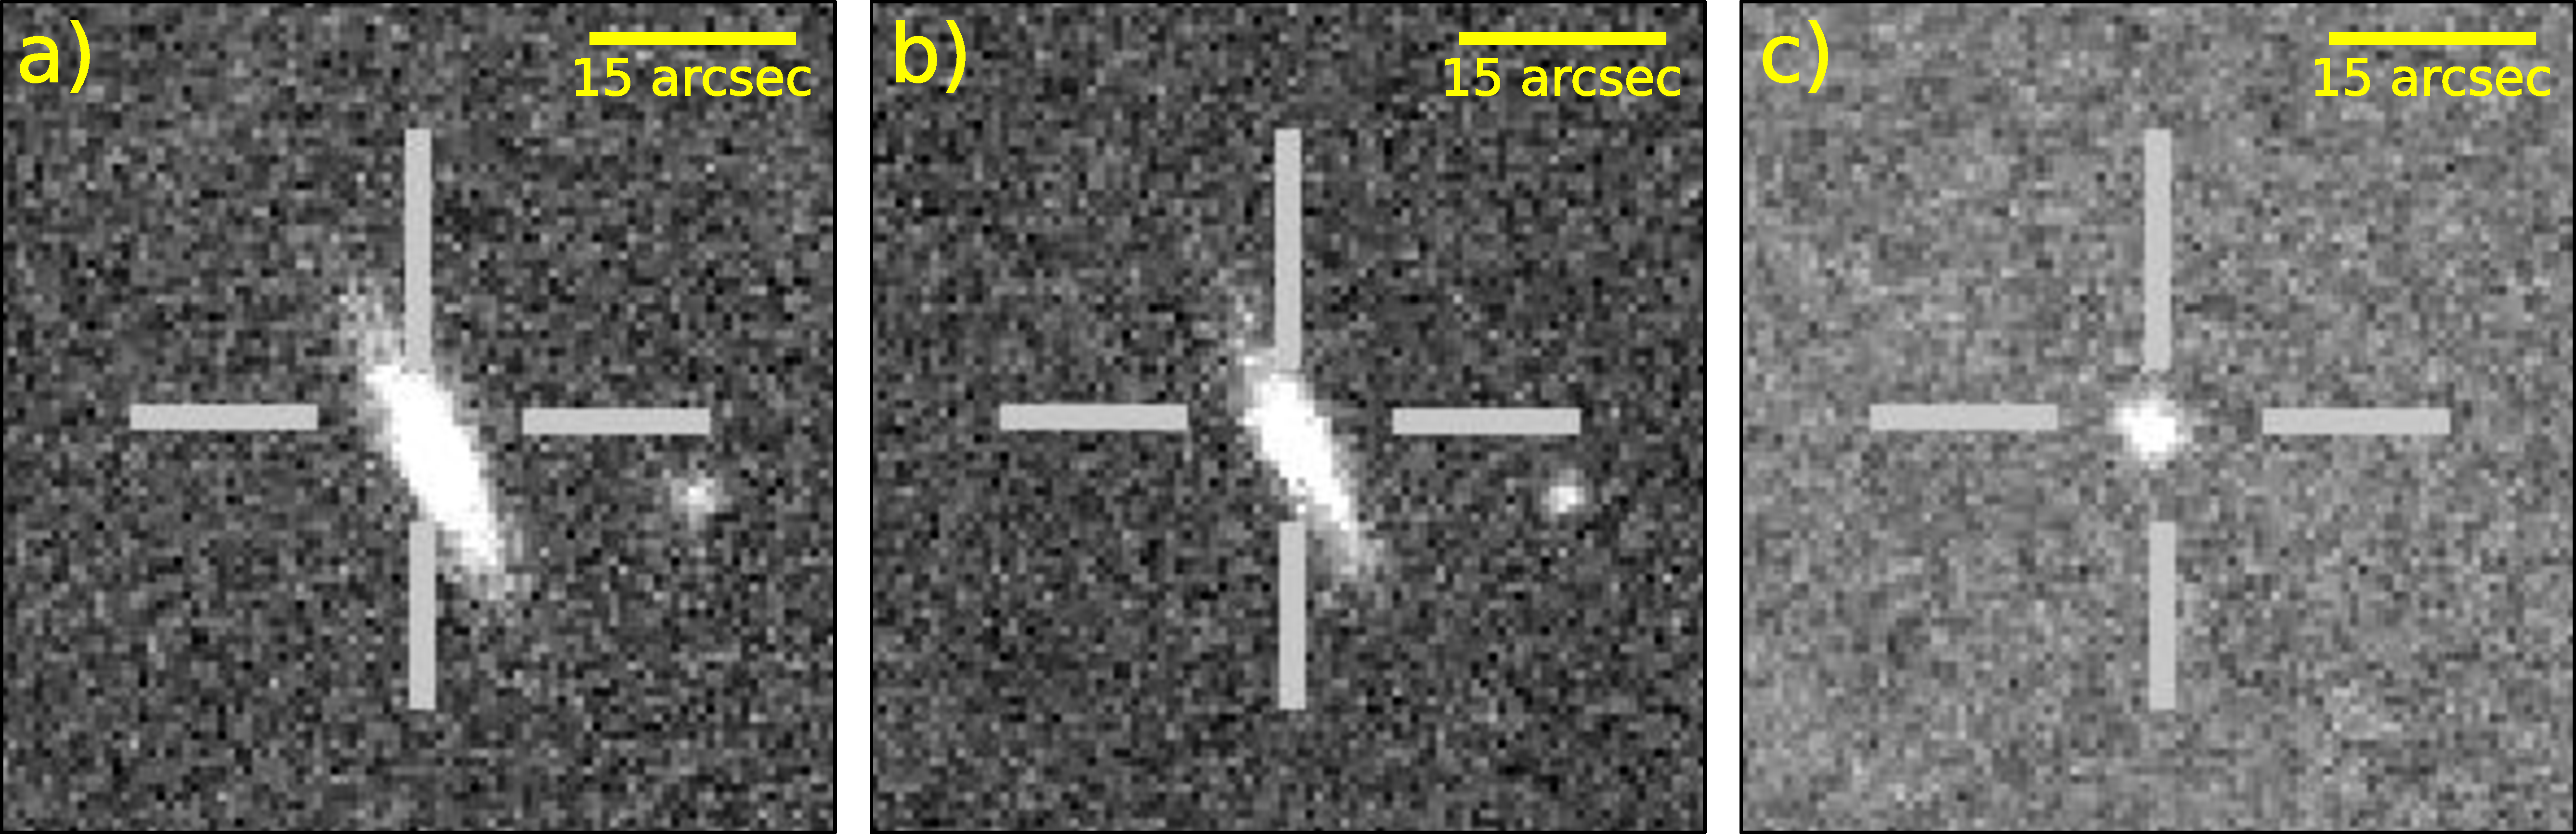
\includegraphics[width=\linewidth]{images/diffimg.pdf}
\caption[The detection of SN 2019bpc through difference imaging]{The detection of Type Ia supernova SN 2019bpc by the GOTOphoto difference imaging pipeline. The new exposure on the left (a) has the reference image (b) subtracted to give the difference image on the right (c), where the new source is clearly visible.}
\label{fig:difference_imaging}
\end{figure}


\end{colsection}

% ~~~~~~~~~~~~~~~~~~~~

\end{colsection}

% ########################################

\newpage
\section{Tiling the sky with GOTO-tile}
\label{sec:gototile}
\begin{colsection}

% ~~~~~~~~~~~~~~~~~~~~

\begin{colsection}

GOTO-tile is a \proglang{Python} module (\pkg{gototile} \rtxt{footnote url?}) created for the \gls{goto} project to contain all the functions and frameworks related to tiling the sky. It was originally developed by Darren White as a way to process \gls{ligo} \gls{gw} skymaps for \gls{goto}, and then maintained by Evert Rol who rearranged it into a module usable for some other telescopes including SuperWASP on La Palma and a proposed southern GOTO node. My contributions to the module have been more fundamental: reworking the foundations to improve how grids are defined and skymaps are applied to them, as well as adding different ways to create skymaps.

\end{colsection}

% ~~~~~~~~~~~~~~~~~~~~

\subsection{Creating sky grids}
\label{sec:grids}
% different ways to make grids
\begin{colsection}

The core of GOTO-tile as it now exists is the \code{SkyGrid} class. This is used to define a sky grid, a collection of `tiles' defined as points on the celestial sphere (\aref{fig:sphere}). These tiles are aligned to the celestial right ascension/declination coordinates, and are designed to create a base framework for observations to be mapped to.

The most important parameter required when defining a sky grid is the field of view of the telescope, which is taken as the size of the tiles that make up the grid. This is defined by giving a width and height value in degrees, meaning the tiles can only be square or rectangular. This is typically fine for the \gls{goto} array, although there was a period when having three \glspl{ut} in an `L'-shape was considered. This was abandoned due mainly to the complexity of tiling the grid based on abstract shapes.

The second parameter required to define a sky grid is the desired overlap between the tiles. This is given as a value between zero and one in both the right ascension and declination directions, with zero meaning no overlap and one meaning all the tiles are completely overlapping (as this would lead to infinite tiles being created in practice the overlap is restricted to no more than $0.9$). This is used to define the spacing between the tile centrers, although exactly how depends on the algorithm used.

As GOTO-tile has been developed the algorithm used to define tile centres has evolved and improved, but the basic method has remained the same:

\begin{enumerate}
    \item Define equally spaced lines of constant declination, separated by the value $\Delta\delta$ (\aref{fig:deltadelta}). These lines are the basis for the grid, which is defined in ``strips'' of tiles. Exactly how $\Delta\delta$ is defined based on the field of view and overlap parameters depends on the algorithm, in particular how to deal with the poles in case $\Delta\delta$ is not a factor of \SI{90}{\degree}.
    \item Once the strips are defined, then each is filled equally spaced points separated by the value $\Delta\alpha$ (\aref{fig:deltaalpha}). This value is constant for each strip but is (in most algorithms) a function of declination ($\Delta\alpha(\delta)$), meaning that moving away from the equator to the poles each strip will contain a reducing number of points.
    \item These points are then defined as the centre of the tiles, the size of which is given by the field of view (\aref{fig:tiledsphere}).
\end{enumerate}

Once the grid has been created it is encapsulated within the GOTO-tile \code{SkyGrid} class. Each tile is defined by a coordinate at its centre, and each is also given a unique name of the form \code{`T0001'}. The grid itself is also given a name formed using the input field of view and overlap parameters, so a grid created with a field of view of \SI{3.7}{\degree}$\times$\SI{4.9}{\degree} and overlap factor of 0.1 (this is the grid used for the \gls{goto} 4-\gls{ut} all-sky survey) is given the name \code{`allsky-3.7x4.9--0.1--0.1'}. In this way a given tile in a given grid can be recreated just from the names, which is used when storing the grid and tile details in the observation database (see \aref{sec:obsdb}). % chktex 29

% ---------

\begin{figure}[p]
\begin{center}
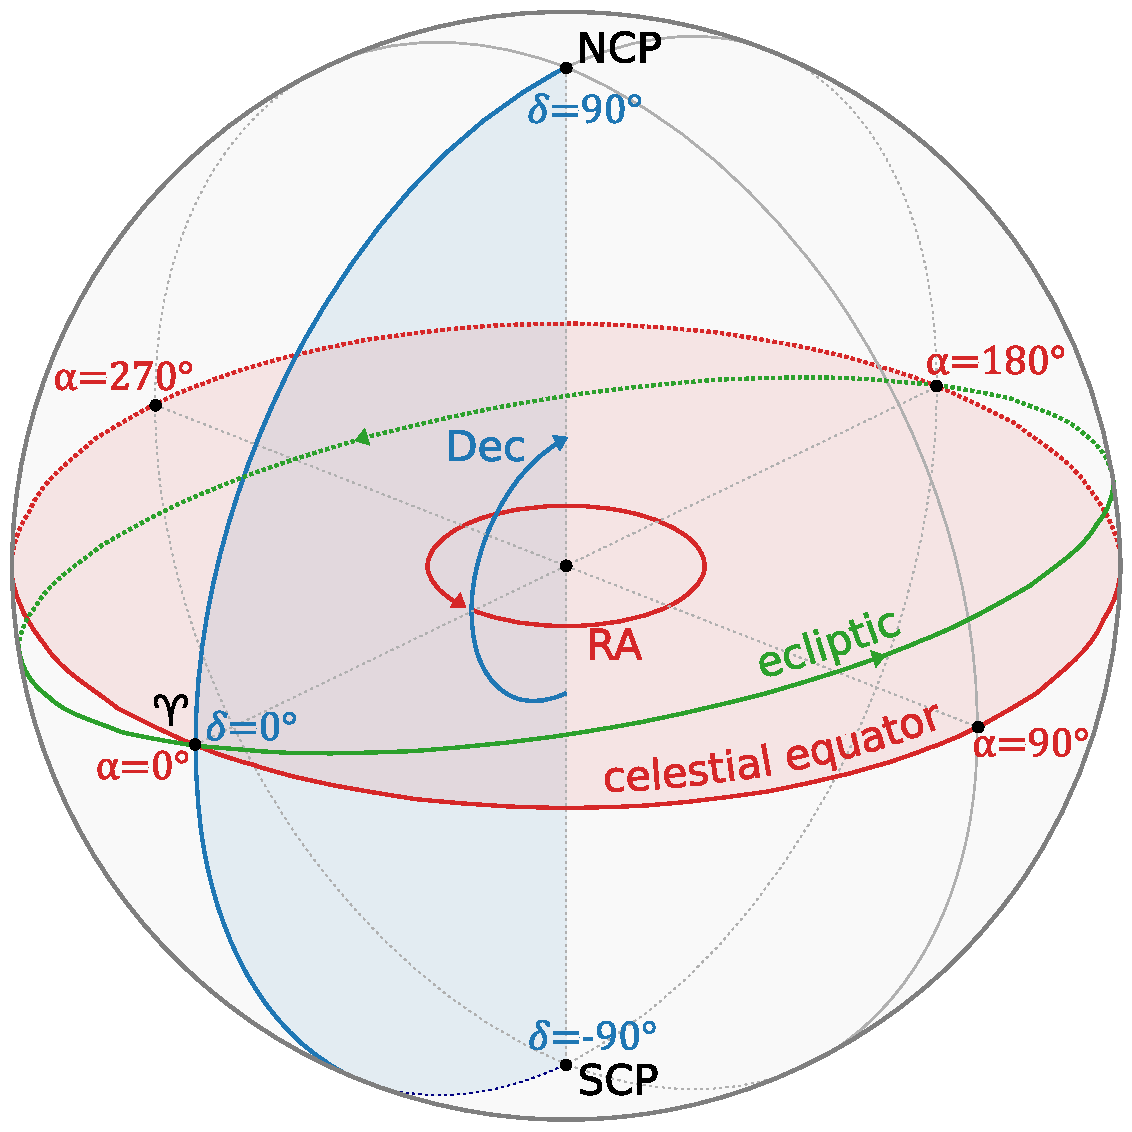
\includegraphics[width=\linewidth]{images/globe1.pdf}
\end{center}
\caption[The celestial sphere]{The celestial sphere. The celestial equator is marked in \textcolor{red}{red}, the vernal equinox (where the ecliptic (not shown) crosses the equator) is marked with the symbol \Aries{} and the meridian that intercepts the vernal equinox is marked in \textcolor{blue}{blue}. The northern and southern celestial poles are marked as NCP and SCP respectively. The definition of the equatorial coordinate system is shown: declination (Dec, $\delta$) is defined as the angle from the equator, ranging from \SI{-90}{\degree} at the SCP to \SI{90}{\degree} at the NCP, and right ascension (RA, $\alpha$) is defined as angle east from the vernal equinox between \SI{0}{\degree} and \SI{360}{\degree}.
}
\label{fig:sphere}
\end{figure}

\begin{figure}[p]
\begin{center}
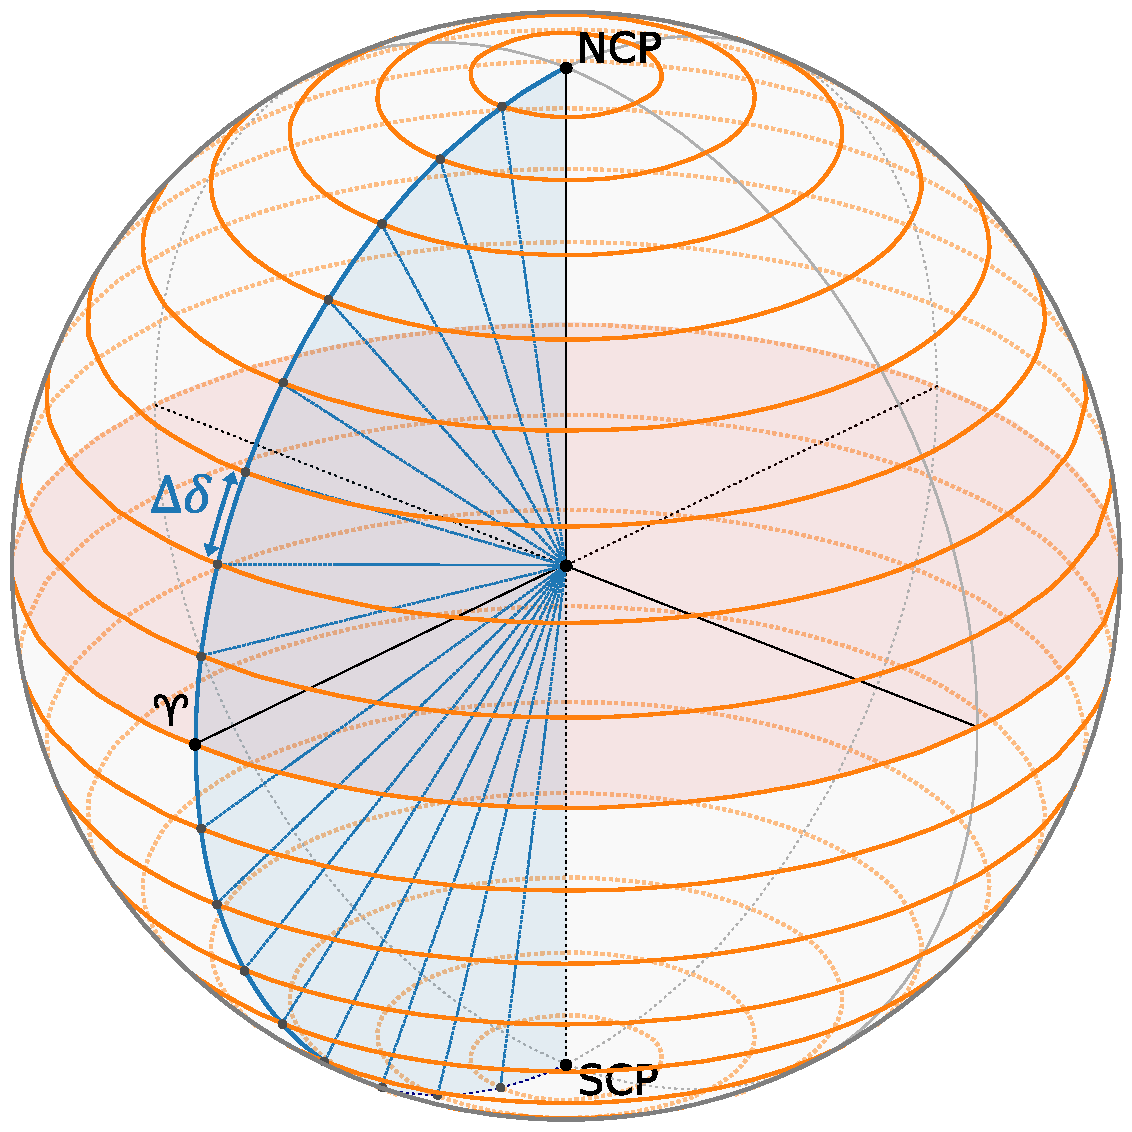
\includegraphics[width=\linewidth]{images/globe2.pdf}
\end{center}
\caption[Defining declination strips]{The first stage when creating a sky grid is defining the declination strips. This is done by dividing the full range of declination (\SI{-90}{\degree} to \SI{90}{\degree}) equally by a constant spacing value $\Delta\delta$. In this example $\Delta\delta =$ \SI{10}{\degree}, and so strips are defined at $\delta=$ \SI{0}{\degree}, \SI{10}{\degree}, \SI{20}{\degree} etc\ldots, and mirrored in the southern hemisphere. There is always a strip with $\delta=0$. Exactly how the strips are defined when $\Delta\delta$ is not an integer factor of \SI{90}{\degree} depends on the algorithm used, in this case using the ``minverlap'' algorithm the strips range from \SI{-90}{\degree} to \SI{90}{\degree} and include a ``strip'' at the poles which will contain single tile (as shown in \aref{fig:tiledsphere}).
}
\label{fig:deltadelta}
\end{figure}

\begin{figure}[p]
\begin{center}
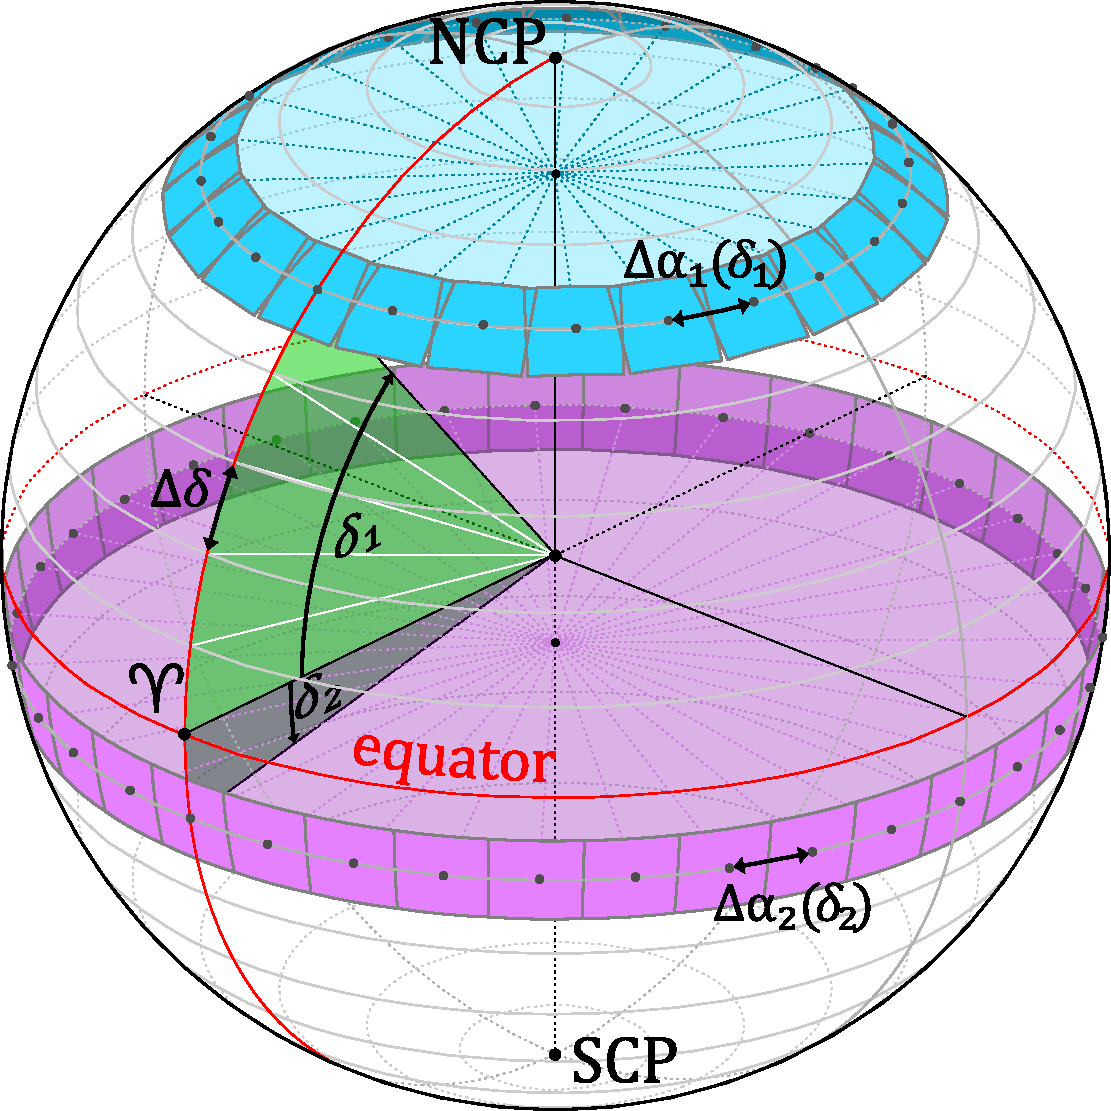
\includegraphics[width=\linewidth]{images/globe3.pdf}
\end{center}
\caption[Defining the spacing between tiles]{After the declination strips are defined (see \aref{fig:deltadelta}) for each strip tile centres are defined with a set spacing $\Delta\alpha(\delta)$. Unlike $\Delta\delta$, which is fixed across the sphere, $\Delta\alpha$ varies as a function of declination meaning strips closer to the poles will contain fewer tiles. Two examples of defining tiles are shown above, one at declination $\delta_1$ (\SI{50}{\degree}, in \textcolor{cyan}{light blue}) in the northern hemisphere and another at $\delta_2$ (\SI{-10}{\degree}, in \textcolor{Plum}{purple}) in the southern hemisphere. The results of the ``minverlap'' algorithm are shown, previous algorithms had different ways of defining $\Delta\alpha$ that would have resulted in different spacings.
}
\label{fig:deltaalpha}
\end{figure}

\begin{figure}[p]
\begin{center}
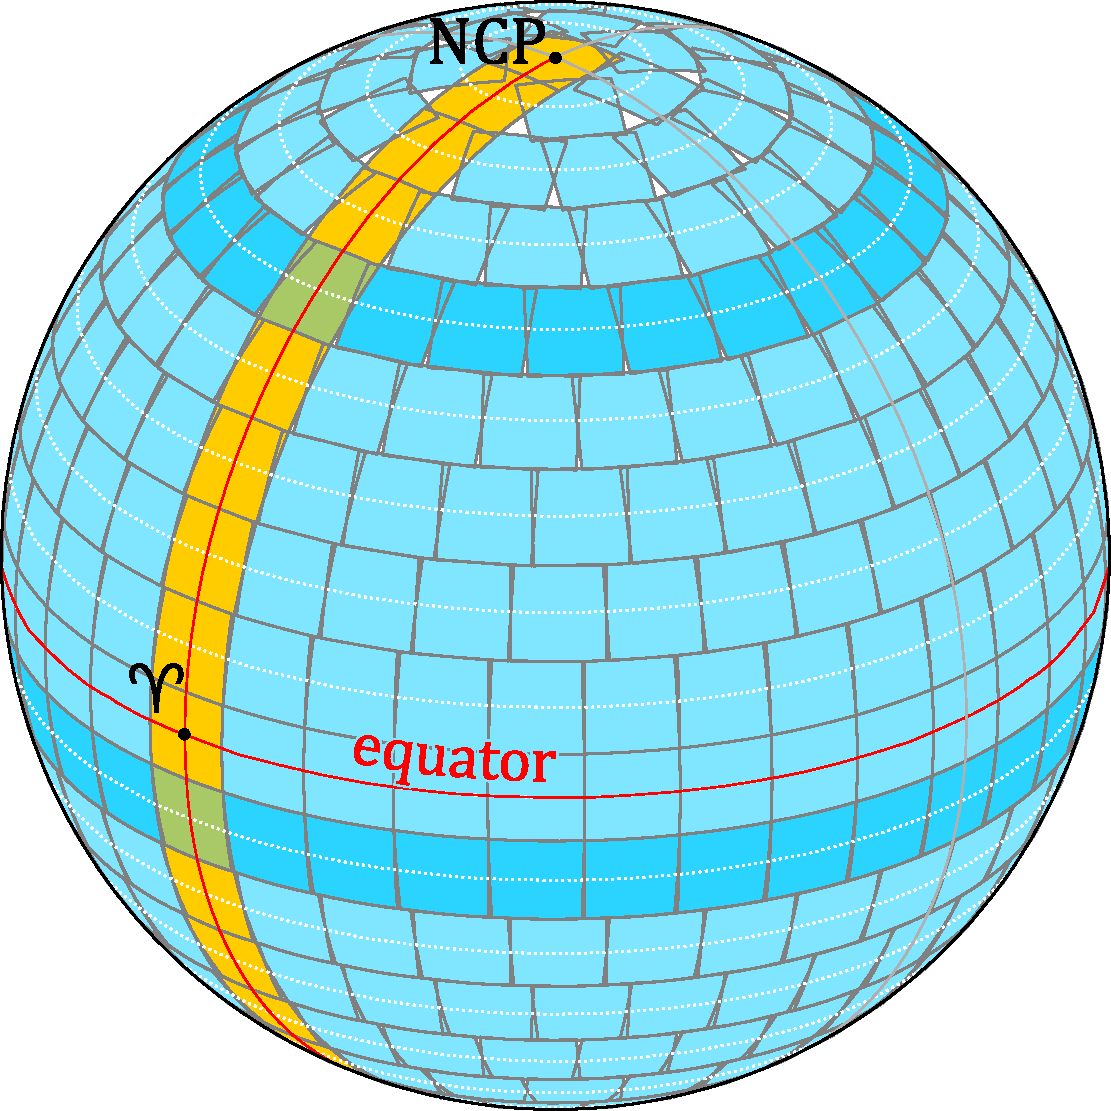
\includegraphics[width=\linewidth]{images/globe4.pdf}
\end{center}
\caption[A fully tiled sphere]{Once every declination strip is complete the full grid is defined, as shown above. The same two strips are shown in \textcolor{cyan}{light blue} and \textcolor{Plum}{purple} as in \aref{fig:deltaalpha}. Due to each strip starting the tile spacing at RA$=0$, there is a fully aligned column of tiles along the vernal equinox, shown in \textcolor{orange}{yellow}. The grid in these examples was defined using the ``minverlap'' algorithm, with each tile having a field of view of \SI{10}{\degree} $\times$ \SI{10}{\degree} and the overlap was set to zero for clarity (note this can lead to gaps between tiles towards the poles, as visible here). In this case the complete grid contains 424 tiles.
}
\label{fig:tiledsphere}
\end{figure}

\newpage

\end{colsection}

% ~~~~~~~~~~~~~~~~~~~~

\subsection{Defining gridding algorithms}
\label{sec:algorithms}
\begin{colsection}

There have been three primary algorithms defined in GOTO-tile's history.

% ---------
\subsubsection{The product algorithm}

The first has since retroactively been called the ``\textbf{product}'' algorithm, and was used when Darren White first wrote GOTO-tile. It first defines the declination step size as

\begin{equation}
    \Delta\delta = f_\text{dec}(1-v_\text{dec}),
    \label{eq:product_deltadelta}
\end{equation}

where $f_\text{dec}$ and $v_\text{dec}$ are respectively the field of view and overlap parameters in the declination direction. The declination strips are then defined by taking steps of this size from the equator towards the poles, stopping when $|\delta| > 90$. The equivalent formula is used to calculate the steps in right ascension

\begin{equation}
    \Delta\alpha = f_\text{RA}(1-v_\text{RA}).
    \label{eq:product_deltaalpha}
\end{equation}

The clear downside of this method is that $\Delta\alpha$ does not vary depending on declination. In effect this algorithm attempts to define the grid as if it was on a flat plane, where the tiles could be arranged in orthogonal rows and columns. In practice when applied to a sphere this leads to a vast number of redundant tiles at the poles, as shown in \aref{fig:product}.

% ---------
\subsubsection{The cosine algorithm}

Due to the obvious problems with the previous algorithm a replacement was written by Evert Rol, which I have since called the ``\textbf{cosine}'' algorithm. It is a more refined version of the ``product'' algorithm, and the declination strips are calculated in the same manor using \aref{eq:product_deltadelta}. However \aref{eq:product_deltaalpha} is modified to depend on declination into

\begin{equation}
    \Delta\alpha(\delta) = \frac{f_\text{RA}(1-v_\text{RA})}{\cos(\delta)}.
    \label{eq:cosine_deltaalpha}
\end{equation}

This produces a much more sensible grid as shown in \aref{fig:cosine}. However there remained an issue of asymmetry: the strips are arranged increasing and decreasing from $\delta=0$ and the tiles are then arranged within the strips starting from $\alpha=0$. As visible in \aref{fig:cosine} this leads to varying overlaps when the the tiles within the strips overlap as $\alpha$ approaches \SI{360}{\degree}. Although more subtle there are similar issues at the north and south poles, and it's common for there to be small gaps between the tiles at high and low declinations.

% ---------
\subsubsection{The minverlap algorithm}

Due to these problems I created a new method to create the grid, called the ``\textbf{minverlap}'' (minimum overlap) algorithm. The same grid created with this algorithm is shown in \aref{fig:minverlap}. The intention of the new algorithm was to solve these issues by adjusting the spacing between tiles to prevent odd gaps. The previous two algorithms both treat the given overlap parameter as as unegotiable, and if the resulting spacings don't give an integer number of tiles within the ranges available then there are uneven gaps at the edges. This is shown more clearly in \aref{fig:cosine_spacing}, where a tricky spacing results in gaps at the poles and variable overlaps on the meridian. The ``minverlap'' algorithm solves this by treating the given overlap parameter not as fixed but as the \textit{minimum} required overlap between tiles. If a grid is requested with an overlap of $0.2$ (20\%), but the odd field of view of the tiles doesn't fit neatly into the ranges then the overlap can be incensed until the tiles fit.

In order to do this mathematically, it is first necessary to find the number of tiles $n$ that would fit into the range using the previous spacing, and then if it isn't an integer number round it up to the next whole number. In declination this is calculated as

\begin{equation}
    n_\text{dec} = \left \lceil \frac{90}{f_\text{dec}(1-v_\text{dec})} \right \rceil,
    \label{eq:minverlap_ndec}
\end{equation}

where $\lceil x \rceil$ is the mathematical ceiling function. This is a modification of the previous \aref{eq:product_deltadelta} but one that will always find an integer number of tiles. For example, with $f_\text{dec} = $ \SI{13}{\degree} and $v_\text{dec} = 0.2$ the previous spacing $\Delta\delta = 13 \times (1-0.2) = $ \SI{10.4}{\degree}. This clearly doesn't divide into the \SI{90}{\degree} range without a remainder, which is \SI{6.8}{\degree} as shown in \aref{fig:cosine_spacing}. The problem is that \SI{90}{\degree} $/$ \SI{10.4}{\degree} $= 8.65$. So the previous algorithms will fit in 8 tiles and have over half a tile remaining at the poles. Instead the minverlap algorithm rounds this up to $n_\text{dec} = 9$ tiles, and then simply calculates the spacing using

\begin{equation}
    \Delta\delta = \frac{90}{n_\text{dec}}.
    \label{eq:minverlap_deltadelta}
\end{equation}

In this case the new $\Delta\delta = $ \SI{10}{\degree}, which gives an even arrangement of tiles from the equator to the poles, as shown in \aref{fig:minverlap_spacing}. The other benefit of this method is that, in addition to there always being a declination strip at $\delta=0$, there will always be ``strips'' at \SI{+90}{\degree} and \SI{-90}{\degree}, which results in a single tile being located covering the poles and ensuring there are no major gaps in coverage.

Right ascension is treated similarly. The integer number of tiles that can fit into a given declination strip is given by

\begin{equation}
    n_\text{RA}(\delta) = \left \lceil \frac{360}{f_\text{RA}(1-v_\text{RA})/\cos(\delta)} \right \rceil + 1,
    \label{eq:minverlap_nra}
\end{equation}

where the $+1$ is here necessary to account for tiles being located both at $\alpha=$\SI{0}{\degree} and $\alpha=$\SI{360}{\degree}. The logic is exactly the same as with declination, and the revised spacing is given by

\begin{equation}
    \Delta\alpha(\delta) = \frac{360}{n_\text{RA}(\delta)}.
    \label{eq:minverlap_deltaalpha}
\end{equation}

The effect of this is also shown in \aref{fig:minverlap_spacing}, and tiles are uniformly spaced around the declination strip. Note here the ceiling function does produce a slight degeneracy in $\Delta\alpha$ being a function of $\delta$. Using the same parameters as the previous example $\Delta\delta=$\SI{10}{\degree}, so declination strips start at \SI{0}{\degree} and continue to \SI{\pm10}{\degree}, \SI{\pm20}{\degree} \ldots (mirrored in both hemispheres). From \aref{eq:minverlap_nra} the number of tiles on the equator is $n_\text{RA}(\delta=\SI{0}{\degree}) = \lceil 360/(10.4/\cos(0)) \rceil + 1 = \lceil 34.6 \rceil + 1 = 36$. But on the next strip up (or down) $n_\text{RA}(\delta=\SI{\pm10}{\degree}) = \lceil 360/(10.4/\cos(\pm10)) \rceil + 1 = \lceil 34.1 \rceil + 1 = 36$ as well. This is a natural occurrence as there are only a limited number of ways to fit an integer number of fixed tiles into a given range, and so as shown in \aref{fig:minverlap} the three strips around the equator align perfectly with the same number of tiles.

% ---------
\subsubsection{Limitations of the minverlap algorithm}

The new ``minverlap'' algorithm is an improvement on the previous versions, in particular as it reduces the occurrences of gaps in coverage closer to the poles that happened when using the ``cosine'' algorithm. However the new algorithm is not perfect and gaps can still occur if the starting overlap parameter is very low. For example, \aref{fig:tiledsphere} shows a sphere tiled using the ``minverlap'' algorithm and an overlap parameter of 0. In this case gaps are visible in the strips of tiles just below the northern celestial pole. A proposed solution to this problem would be to force tiles to meet at their lower corners (in the northern hemisphere, upper corners in the south), therefore overlapping further and removing the possibility of gaps forming due to the angle between the tiles. An attempt to make this change and create an ``enhanced minverlap'' algorithm was tested, however ultimately it proved unnecessary. Although the current algorithm is deficient at low overlap values, this is only an issue for large tiles and very low overlaps. The \SI{10}{\degree} $\times$ \SI{10}{\degree} tiles and 0\% overlap used for \aref{fig:tiledsphere} are extreme values, and even for the roughly \SI{8}{\degree} $\times$ \SI{5}{\degree} full field of view of a full GOTO telescope the overlap has to be less than 10\% before noticeable gaps start appearing. As well, from the site on La Palma the northern celestial pole is actually below \glspl{goto} nominal horizon of \SI{30}{\degree}, therefore meaning tiles close to the pole will never be visible and the gaps in coverage were irrelevant. Should GOTO-tile be applied in the future to other projects then this issue would need to be revisited, but it was not a priority to fix within the context of this work.

% ---------

\begin{figure}[p]
\begin{minipage}[c]{0.46\textwidth}
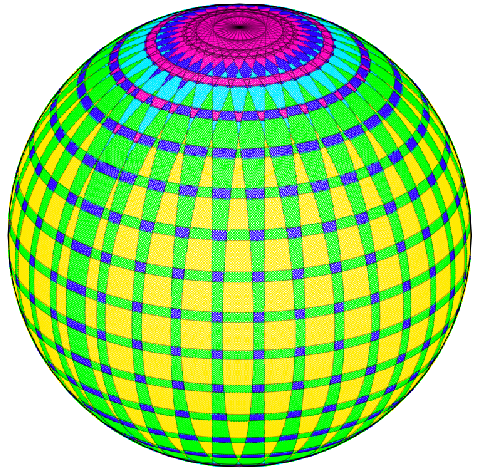
\includegraphics[width=\linewidth]{images/algo_product.pdf}
\end{minipage}
\hfill
\begin{minipage}[c]{0.50\textwidth}
\caption[The ``product'' gridding algorithm]{A sky grid of tiles defined using the ``product'' gridding algorithm. The inputs were a field of view of \SI{13}{\degree} $\times$ \SI{13}{\degree} and an overlap factor of $0.2$ in both axes. The colours show overlapping coverage: \textcolor{Yellow}{yellow} areas are within only one tile, \textcolor{green}{green} two, \textcolor{blue}{blue} three, \textcolor{cyan}{cyan} four and \textcolor{RubineRed}{pink} five or more. This grid contains 595 tiles. Note the constant spacing of tiles in RA and the huge number of redundant tiles at the pole.}
\label{fig:product}
\end{minipage}
\end{figure}

\begin{figure}[p]
\begin{minipage}[c]{0.50\textwidth}
\caption[The ``cosine'' gridding algorithm]{A sky grid of tiles defined using the ``product'' gridding algorithm. The input parameters and colours are the same as in \aref{fig:product}. This grid contains 393 tiles. Note the asymmetric ``seam'' along the $\alpha=0$ meridian, and the \textcolor{red}{red} areas near the pole that are not within the area of any tiles.}
\label{fig:cosine}
\end{minipage}
\hfill
\begin{minipage}[c]{0.46\textwidth}
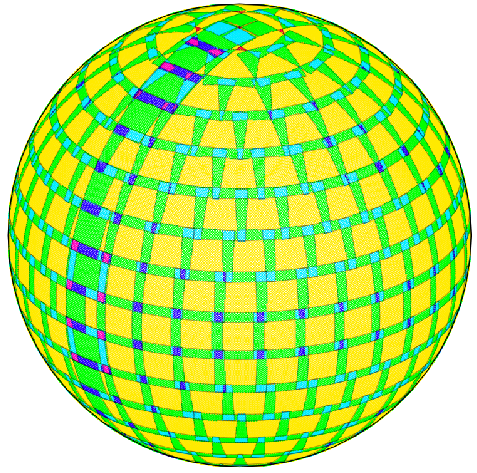
\includegraphics[width=\linewidth]{images/algo_cosine.pdf}
\end{minipage}
\end{figure}

\begin{figure}[p]
\begin{minipage}[c]{0.46\textwidth}
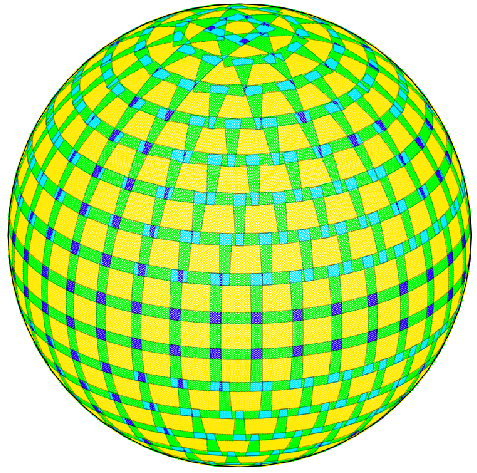
\includegraphics[width=\linewidth]{images/algo_minverlap.pdf}
\end{minipage}
\hfill
\begin{minipage}[c]{0.50\textwidth}
\caption[The ``minverlap'' gridding algorithm]{A sky grid of tiles defined using the ``minverlap'' gridding algorithm. The input parameters and colours are the same as in \aref{fig:product}. This grid contains 407 tiles.  Note the even spacing of tiles even over the $\alpha=0$ meridian, and the better coverage at the pole.}
\label{fig:minverlap}
\end{minipage}
\end{figure}

% ---------

\begin{figure}[p]
\begin{center}
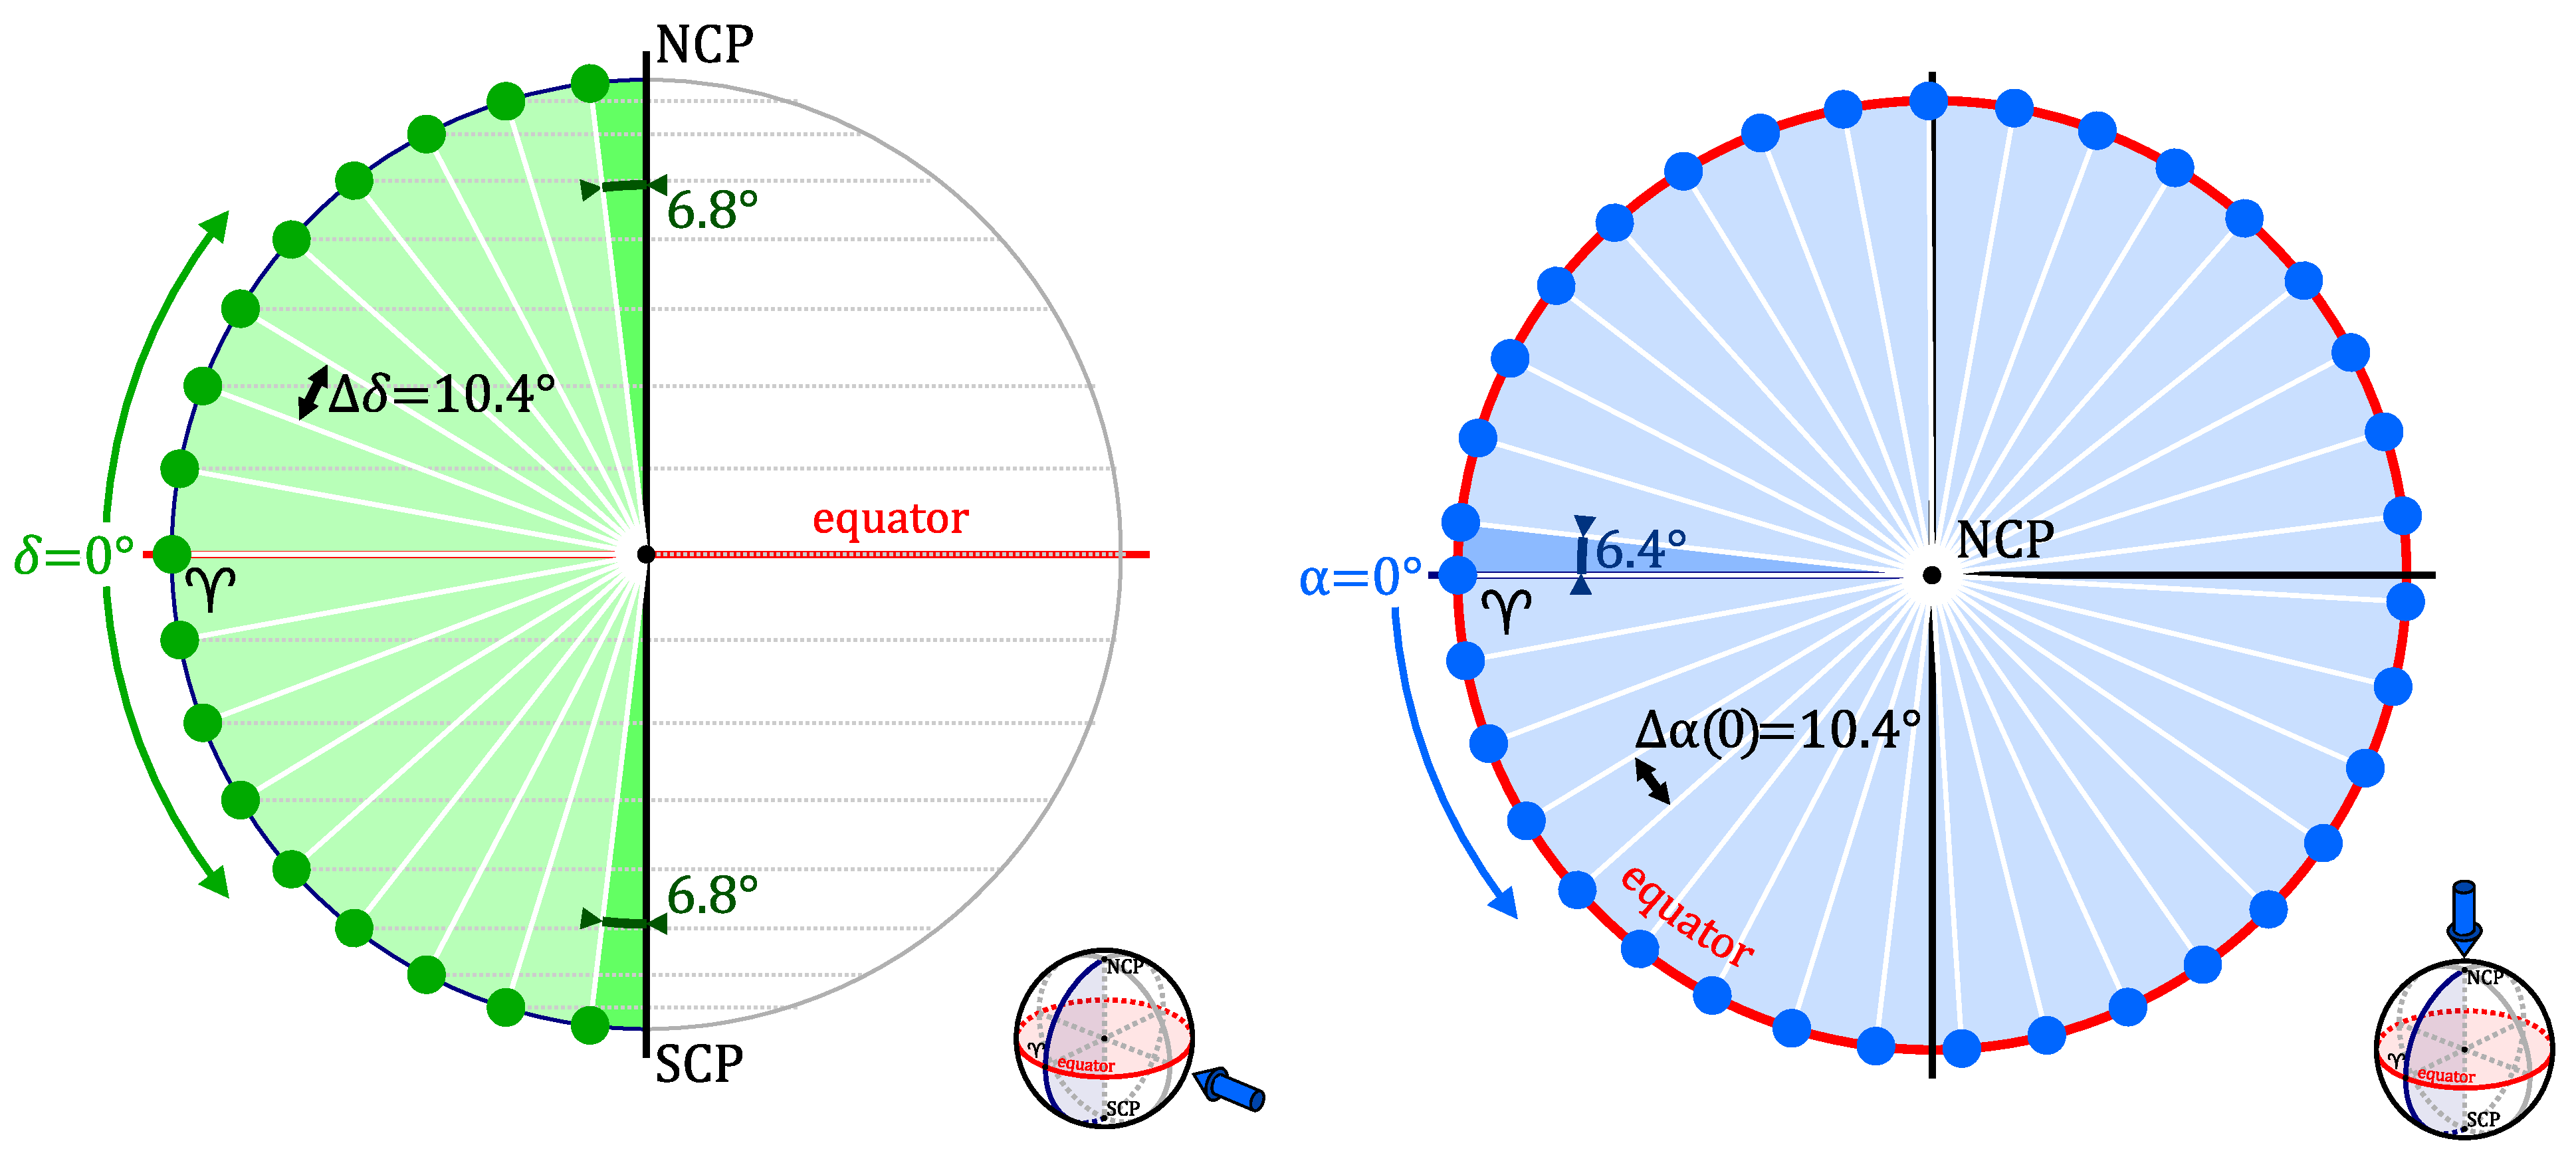
\includegraphics[width=\linewidth]{images/spacing_cosine.pdf}
\end{center}
\caption[Tile spacing with the ``cosine'' algorithm]{Tile spacing with the ``cosine'' algorithm, with a \SI{13}{\degree}$\times$\SI{13}{\degree} FoV and $0.2$ overlap.
\\
\textbf{Left}: \aref{eq:product_deltadelta} gives $\Delta\delta = $ \SI{10.4}{\degree}, which does not divide into \SI{90}{\degree} without a remainder. 17 strips are defined moving away from $\delta=0$, with last being \SI{6.8}{\degree} from the poles. As this is less than half of the field of view (\SI{6.5}{\degree}) the poles themselves will not fall within the area of any tile.
\\
\textbf{Right}: \aref{eq:cosine_deltaalpha} gives $\Delta\alpha = $ \SI{10.4}{\degree} on the equator ($\delta=0$). This results in 35 tiles and a reduced spacing of \SI{6.4}{\degree} to the west of the $\alpha=0$ meridian. This remainder will be different for each strip as $\delta$ changes, as visible in \aref{fig:cosine}.
}
\label{fig:cosine_spacing}
\end{figure}

\begin{figure}[p]
\begin{center}
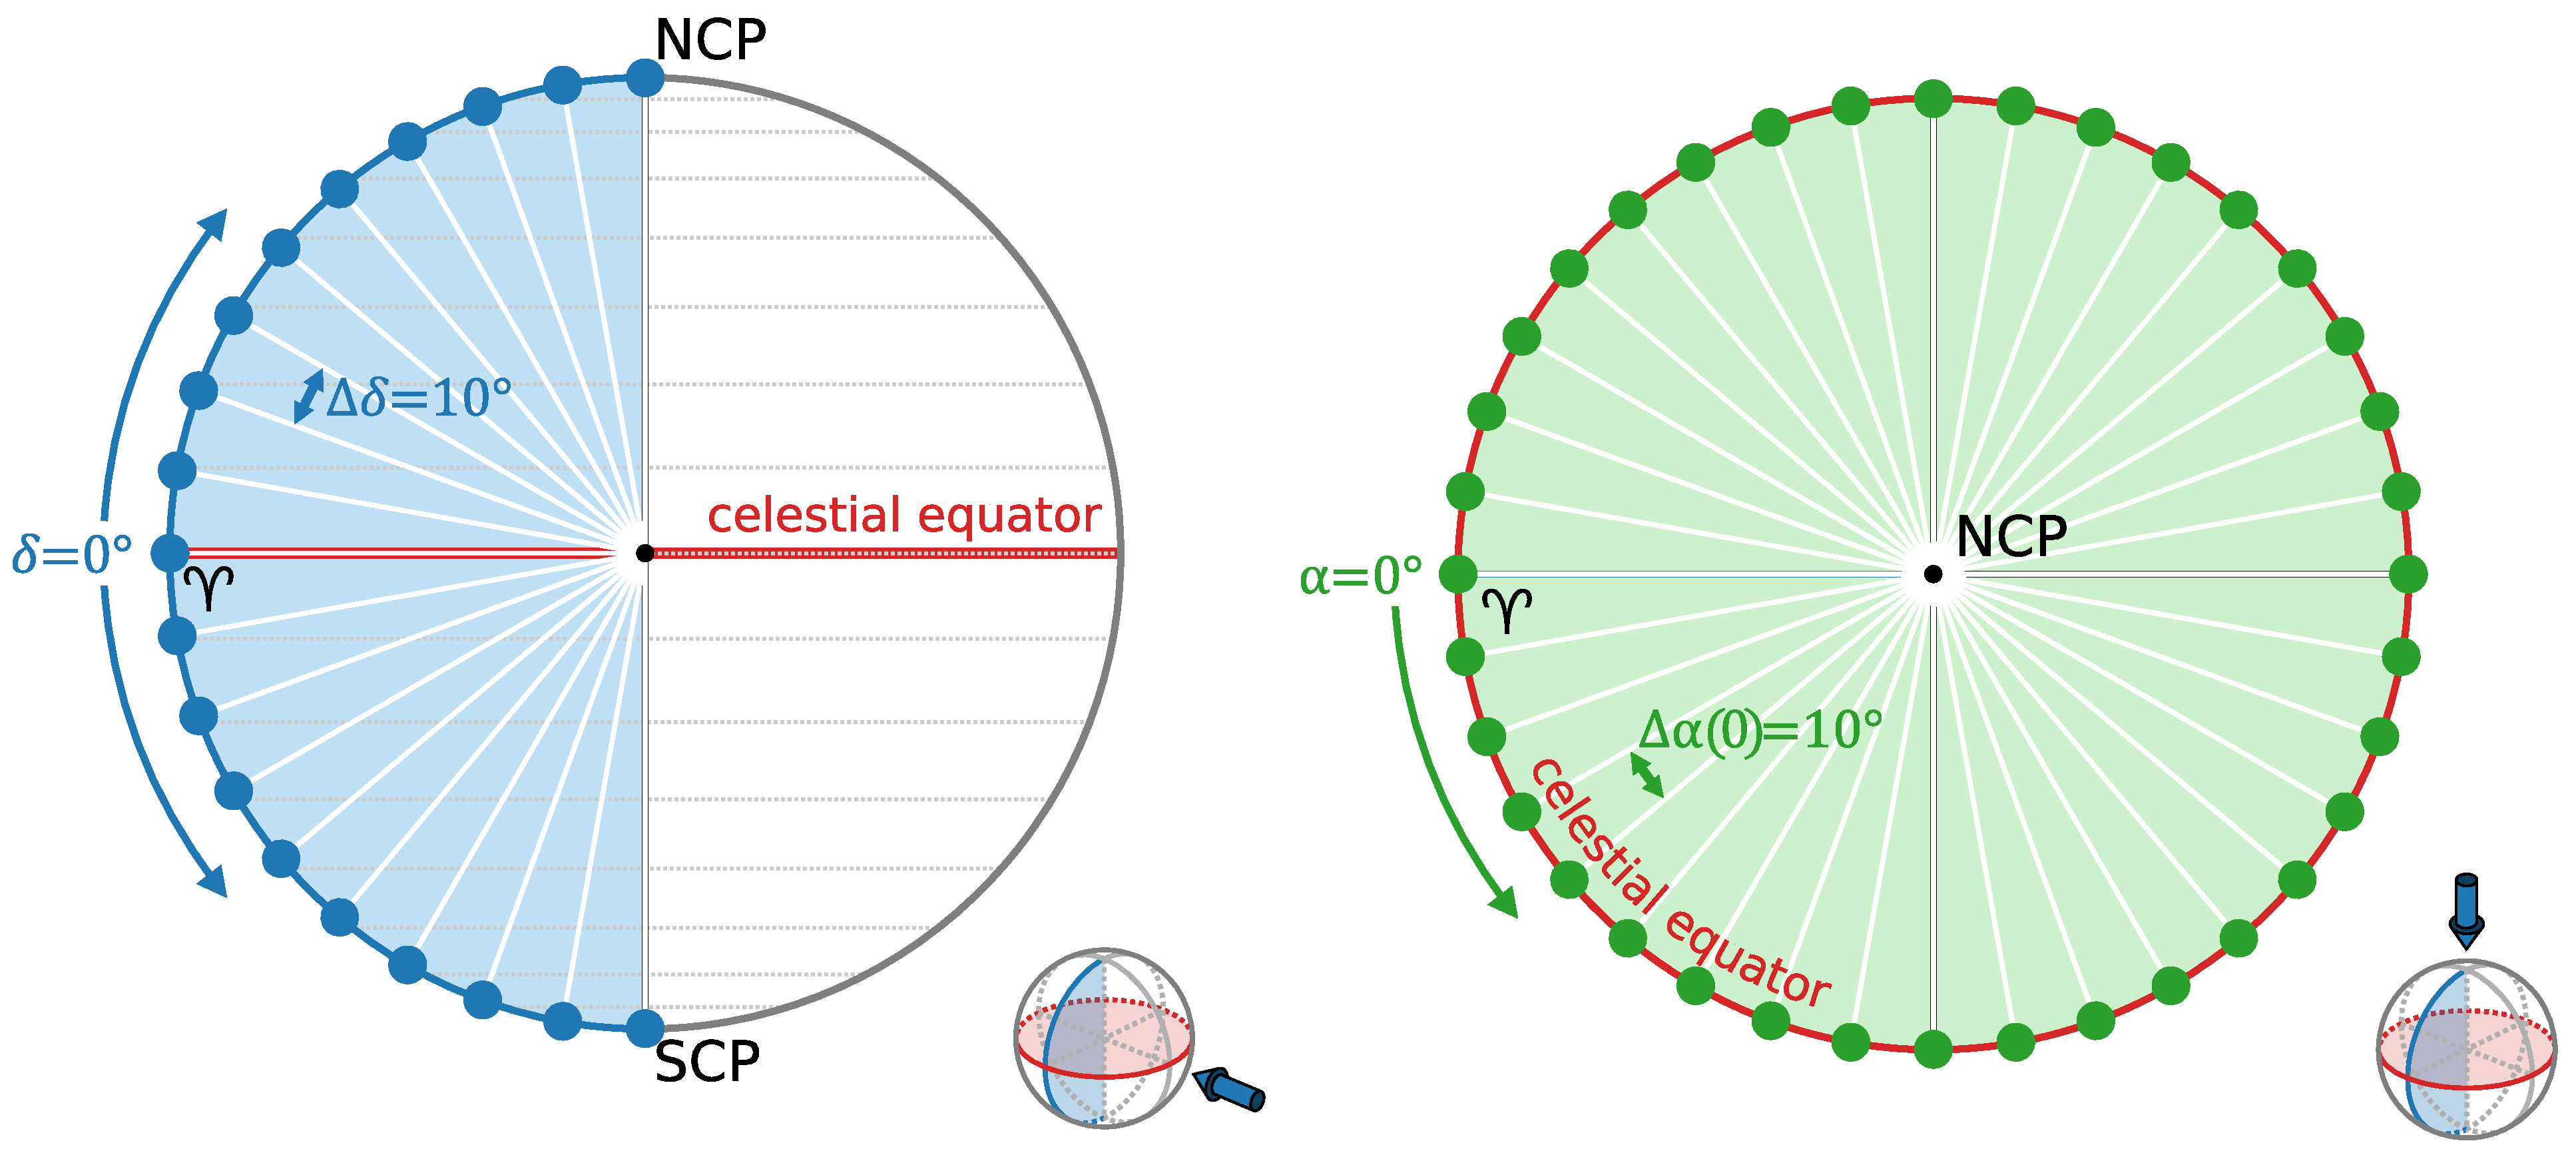
\includegraphics[width=\linewidth]{images/spacing_minverlap.pdf}
\end{center}
\caption[Tile spacing with the ``minverlap'' algorithm]{Tile spacing with the ``minverlap'' algorithm, with the same parameters as \aref{fig:cosine_spacing}.
\\
\textbf{Left:} \aref{eq:minverlap_deltadelta} gives $\Delta\delta = $ \SI{10}{\degree}, therefore neatly arranging 19 strips between \SI{-90}{\degree} and \SI{90}{\degree}.
\\
\textbf{Right:} \aref{eq:minverlap_deltaalpha} also gives $\Delta\alpha = $ \SI{10}{\degree} on the equator ($\delta=0$), so 36 tiles are uniformly arranged around the circumference of the sphere.
}
\label{fig:minverlap_spacing}
\end{figure}

\newpage

\end{colsection}

% ~~~~~~~~~~~~~~~~~~~~

\subsection{HEALPix and probability skymaps}
\label{sec:skymaps}
\begin{colsection}

\gls{healpix} is a system used to define pixelised data on the surface of a sphere~\citep{HEALPix}. Developed at NASA JPL for microwave background data, it is now widely used for other applications including for gravitational wave skymaps produced by the \gls{lvc}. HEALPix divides the sphere into a series of nested (hierarchical) equal-area (although not equal-shape) pixels arranged in declination strips (``isoLatitude''). Shown in \aref{fig:healpix} are the first four orders of spheres, starting from a base resolution with 12 pixels and increasing as each pixel is split into four. The resolution of the sphere is defined using the $N_\text{side}$ parameter, which is given by the number of pixels along the side of one of the 12 base pixels in the given resolution. At every resolution each base-resolution pixel contains $N_\text{side}^2$ pixels, so the total number of pixels in a sphere is given by

\begin{equation}
    N_\text{pix} = 12 N_\text{side}^2.
    \label{eq:healpix_npix}
\end{equation}

Each pixel therefore has an equal area of

\begin{equation}
    \Omega_\text{pix} = \frac{4\pi}{12 N_\text{side}^2} = \frac{\pi}{3 N_\text{side}^2},
    \label{eq:healpix_area}
\end{equation}

on a unit sphere where the radius $r=1$. Taking the celestial sphere, the circumference in degrees is $\SI{360}{\degree} = 2 \pi r$ meaning the area of the whole sky is given by

\begin{equation}
    A_\text{sky} = 4 \pi r^2 = 4 \pi \left ( \frac{\SI{360}{\degree}}{2 \pi} \right )^2 = \frac{129600}{\pi}~\text{sq deg} \approx 41252~\text{sq deg} , %chktex 3
    \label{eq:sky_area}
\end{equation}

and therefore the area of each HEALPix pixel is

\begin{equation}
    A_\text{pix} = \frac{129600}{12 \pi N_\text{side}^2}~\text{sq~deg} \approx \frac{3438}{N_\text{side}^2}~\text{sq~deg}.
    \label{eq:healpix_area_degrees}
\end{equation}

\aref{fig:healpix} shows only the first four orders of HEALPix pixelisation, up to $N_\text{side} = 8$ where the sphere is split into 768 pixels each with an area (which can be considered the resolution of the grid) of 53.7~sq deg. An initial, low-resolution \gls{lvc} skymap might use a grid with $N_\text{side} = 64$ (49 thousand pixels) and resolution (pixel area) of 0.84~sq~deg, where as a final output skymap will have $N_\text{side} = 1024$, 12.5 million pixels and a resolution of $3.27 \times 10^{-3}$~sq~deg (11.7 square arcminutes).

% ---------

\begin{figure}[t]
\begin{center}
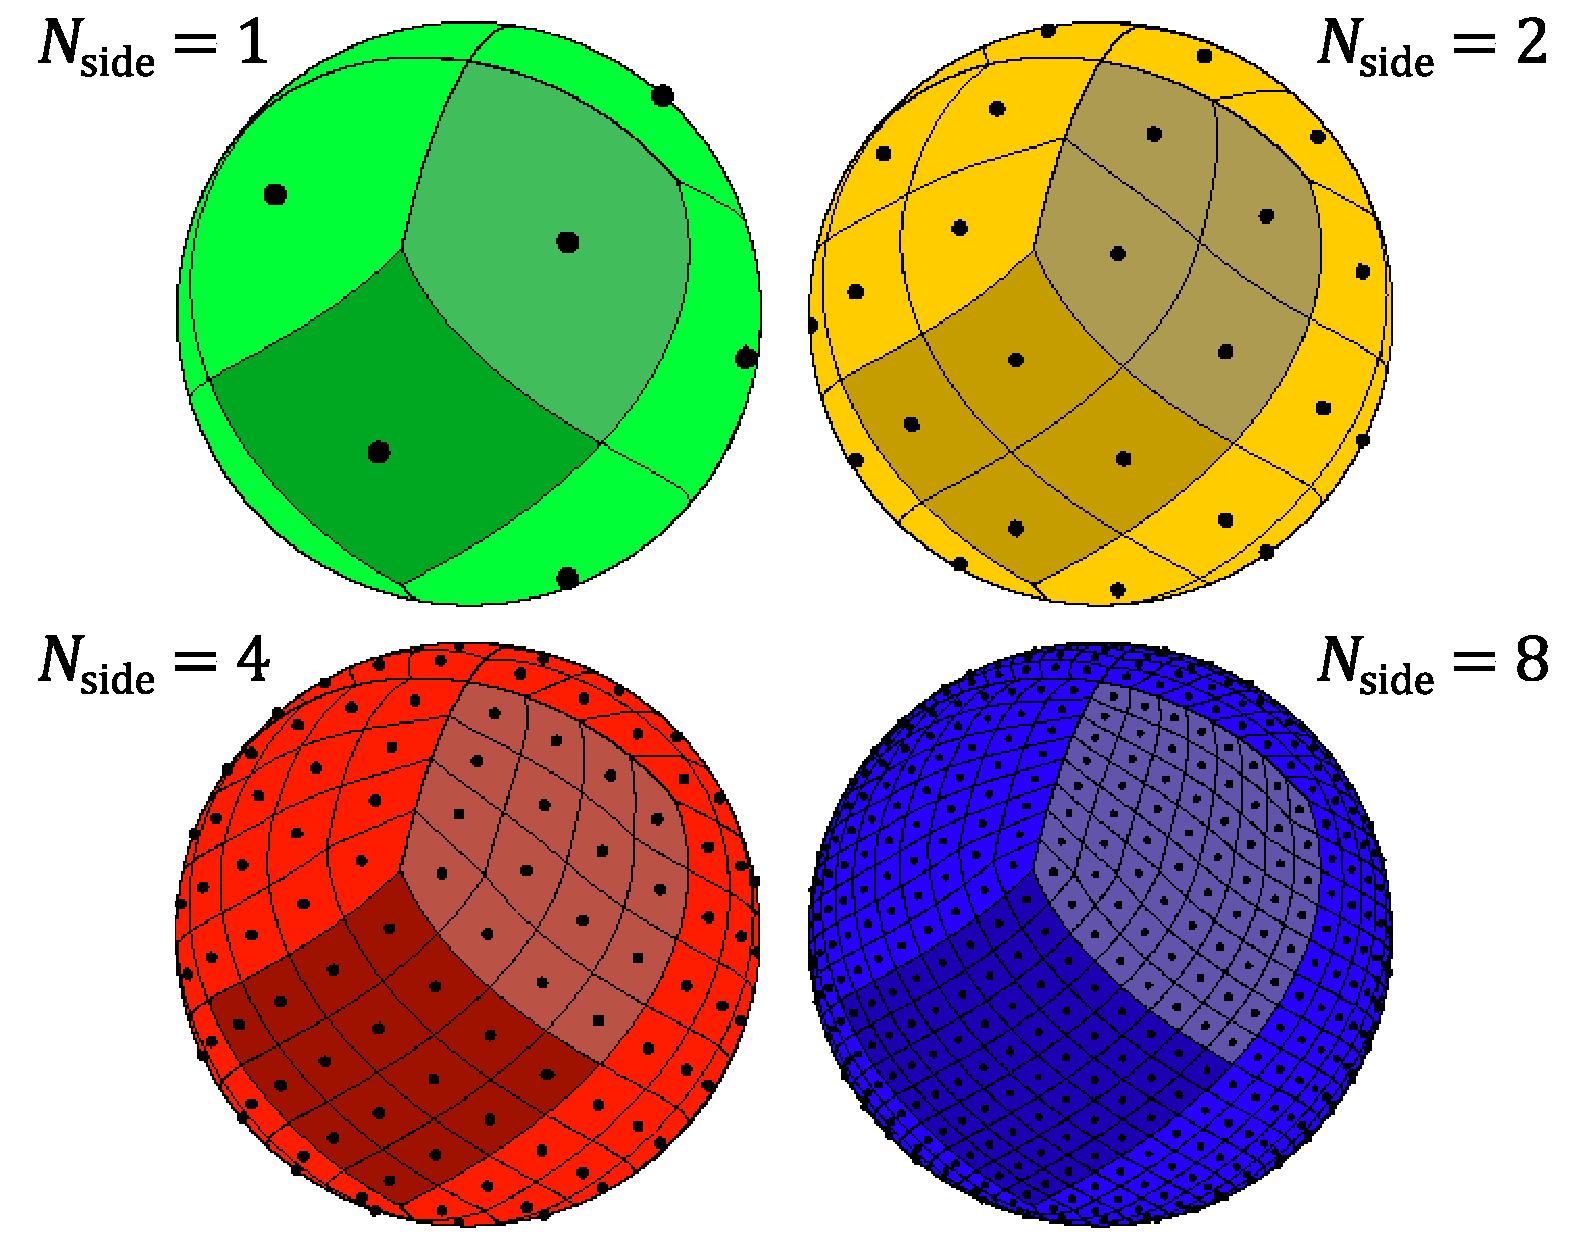
\includegraphics[width=0.7\linewidth]{images/healpix.pdf}
\end{center}
\caption[HEALPix partitions of a sphere]{HEALPix partitions of a sphere, of increasing order and $N_\text{side}$ resolution parameter. Note that as the resolution increases each pixel on the previous sphere is split into four on the new sphere, and $N_\text{side}$ is the number of pixels along the side of a base-resolution pixel (two of which are highlighted). Adapted (colourised) from Figure~4 of \citet{HEALPix}.
}
\label{fig:healpix}
\end{figure}

% ---------

In addition to being a way to divide the sphere, each HEALPix pixel has a unique index from one of two different numbering schemes: either the ring (counting around each ring from the north to the south) or nested (based on the sub-pixel tree) system.

HEALPix is used to provide localisation of sky probabilities for transient astronomical events, in the form of ``skymaps''. Each point on the HEALPix grid is assigned a probability between 0 and 1 that the counterpart object is located within that pixel, and the whole sphere should sum to unity. \aref{fig:skymap_regrade} shows an example \gls{lvc} skymap, for the gravitational wave event S190521r, at various HEALPix $N_\text{side}$ parameters.

% ---------

\begin{figure}[p]
\begin{center}

\begin{tabular}{cc}

$N_\text{side} = 1$: &
$N_\text{side} = 2$:
\\

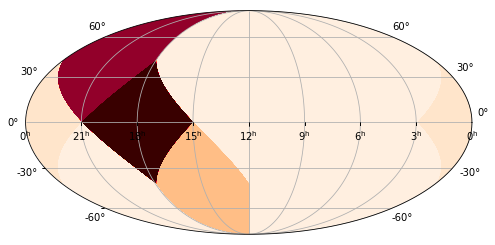
\includegraphics[width=0.45\linewidth]{images/regrade/1.png} &
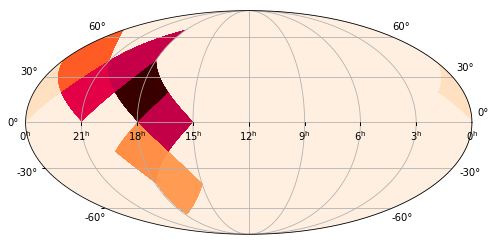
\includegraphics[width=0.45\linewidth]{images/regrade/2.png}
\\
\\

$N_\text{side} = 4$: &
$N_\text{side} = 8$:
\\

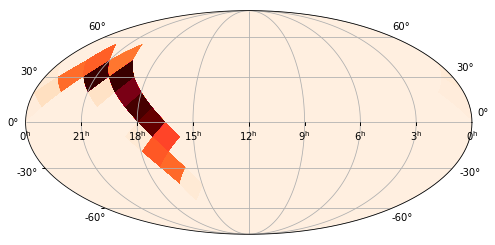
\includegraphics[width=0.45\linewidth]{images/regrade/4.png} &
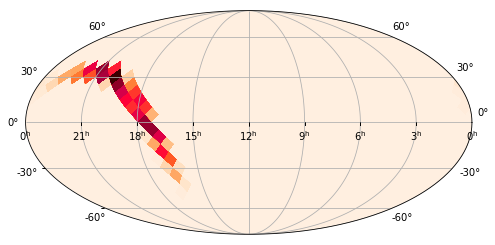
\includegraphics[width=0.45\linewidth]{images/regrade/8.png}
\\
\\

$N_\text{side} = 16$: &
$N_\text{side} = 32$:
\\

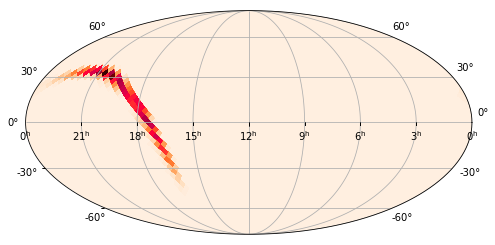
\includegraphics[width=0.45\linewidth]{images/regrade/16.png} &
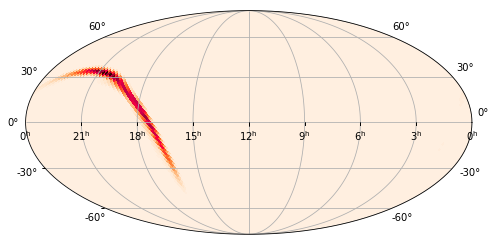
\includegraphics[width=0.45\linewidth]{images/regrade/32.png}
\\
\\

$N_\text{side} = 64$: &
$N_\text{side} = 128$:
\\

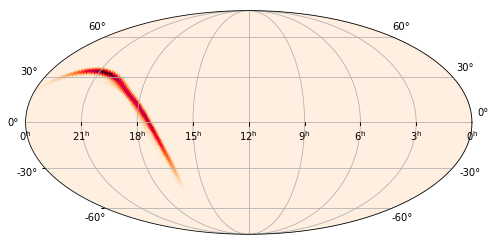
\includegraphics[width=0.45\linewidth]{images/regrade/64.png} &
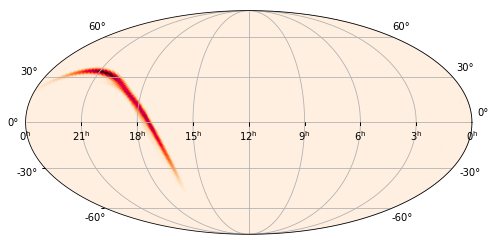
\includegraphics[width=0.45\linewidth]{images/regrade/128.png}
\\

\end{tabular}

\end{center}

\caption[Regrading a gravitational wave skymap]{Changing the HEALPix resolution of a gravitational wave skymap (also known as regrading). At every stage each pixel is assigned a probability value as shown by the colour scale, which indicates the probability the source is located within that pixel. At lower $N_\text{side}$ individual pixels are visible, but as the resolution increases the structure is less visible.
}
\label{fig:skymap_regrade}
\end{figure}

% ---------

\clearpage

As well as the individual probabilities assigned to each pixel, it is also useful to consider the overall spread of the probability. This is done by considering the probability contour areas, typically at the 50\% and 90\% levels. The 50\% contour area of a skymap is defined by encircling the smallest number of pixels so that the total probability within the area is 50\% of the overall skymap probability. When a skymap is defined using GOTO-tile as well as the individual probability values each pixel also has a contour value. This is calculated by sorting all the pixels by probability from highest to lowest, the contour value for each pixel is then cumulative sum of the probability within the pixels above it. This contour value can be considered as the lowest contour area that each pixel is within, meaning the pixels that are contained within the 50\% contour area are those with contour values of less than 50\%. \aref{fig:sim_skymap_probs} and \aref{fig:sim_skymap_conts} illustrate how the contours are calculated for an cartoon 2-dimensional skymap.

% -----

\begin{figure}[p]
\begin{center}

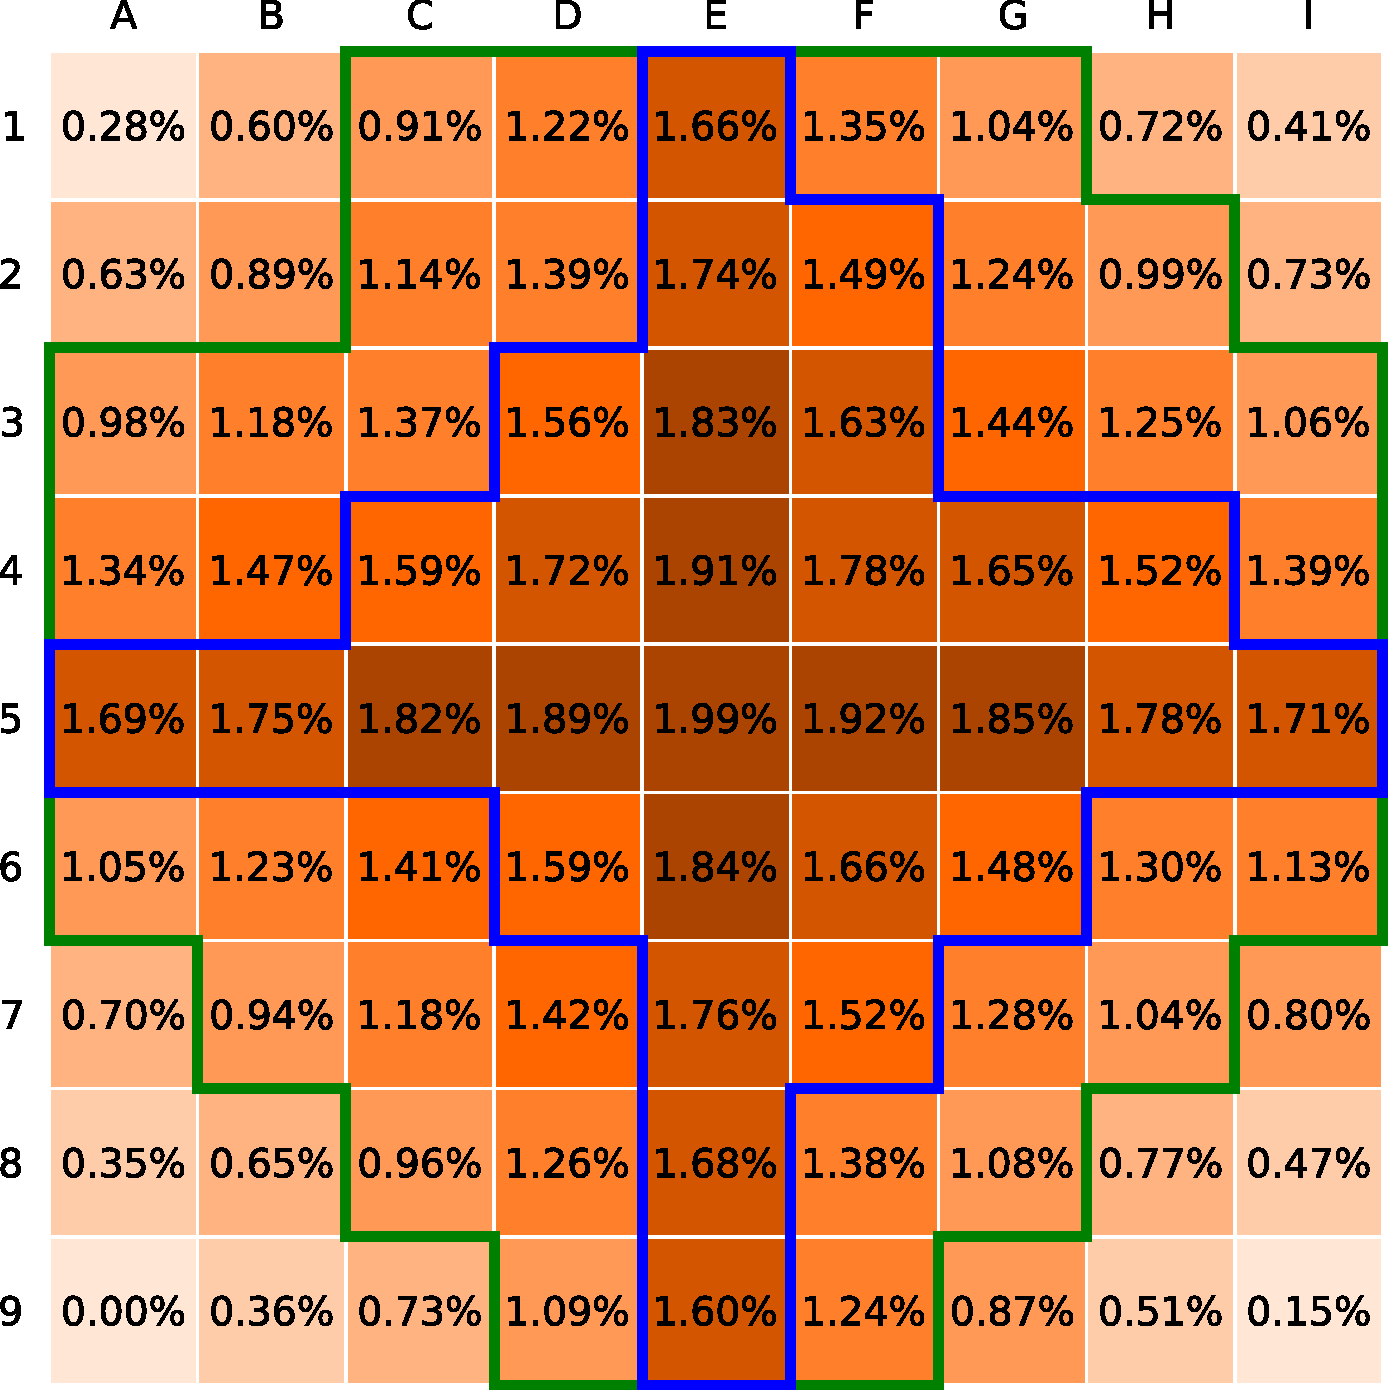
\includegraphics[width=0.95\linewidth]{images/sim/sim_skymap_probs.pdf}

\end{center}

\caption[An example 2D probability skymap]{A cartoon 2-dimensional skymap. Each pixel (represented by one of the 81 squares) has an assigned probability, and together they all sum to 100\%. The inner blue thick contour line contains 50\% of the probability, while the outer green contour line contains 90\% of the probability. These contours are created based on the values shown in \aref{fig:sim_skymap_conts}.
}
\label{fig:sim_skymap_probs}
\end{figure}

% -----

\begin{figure}[p]
\begin{center}

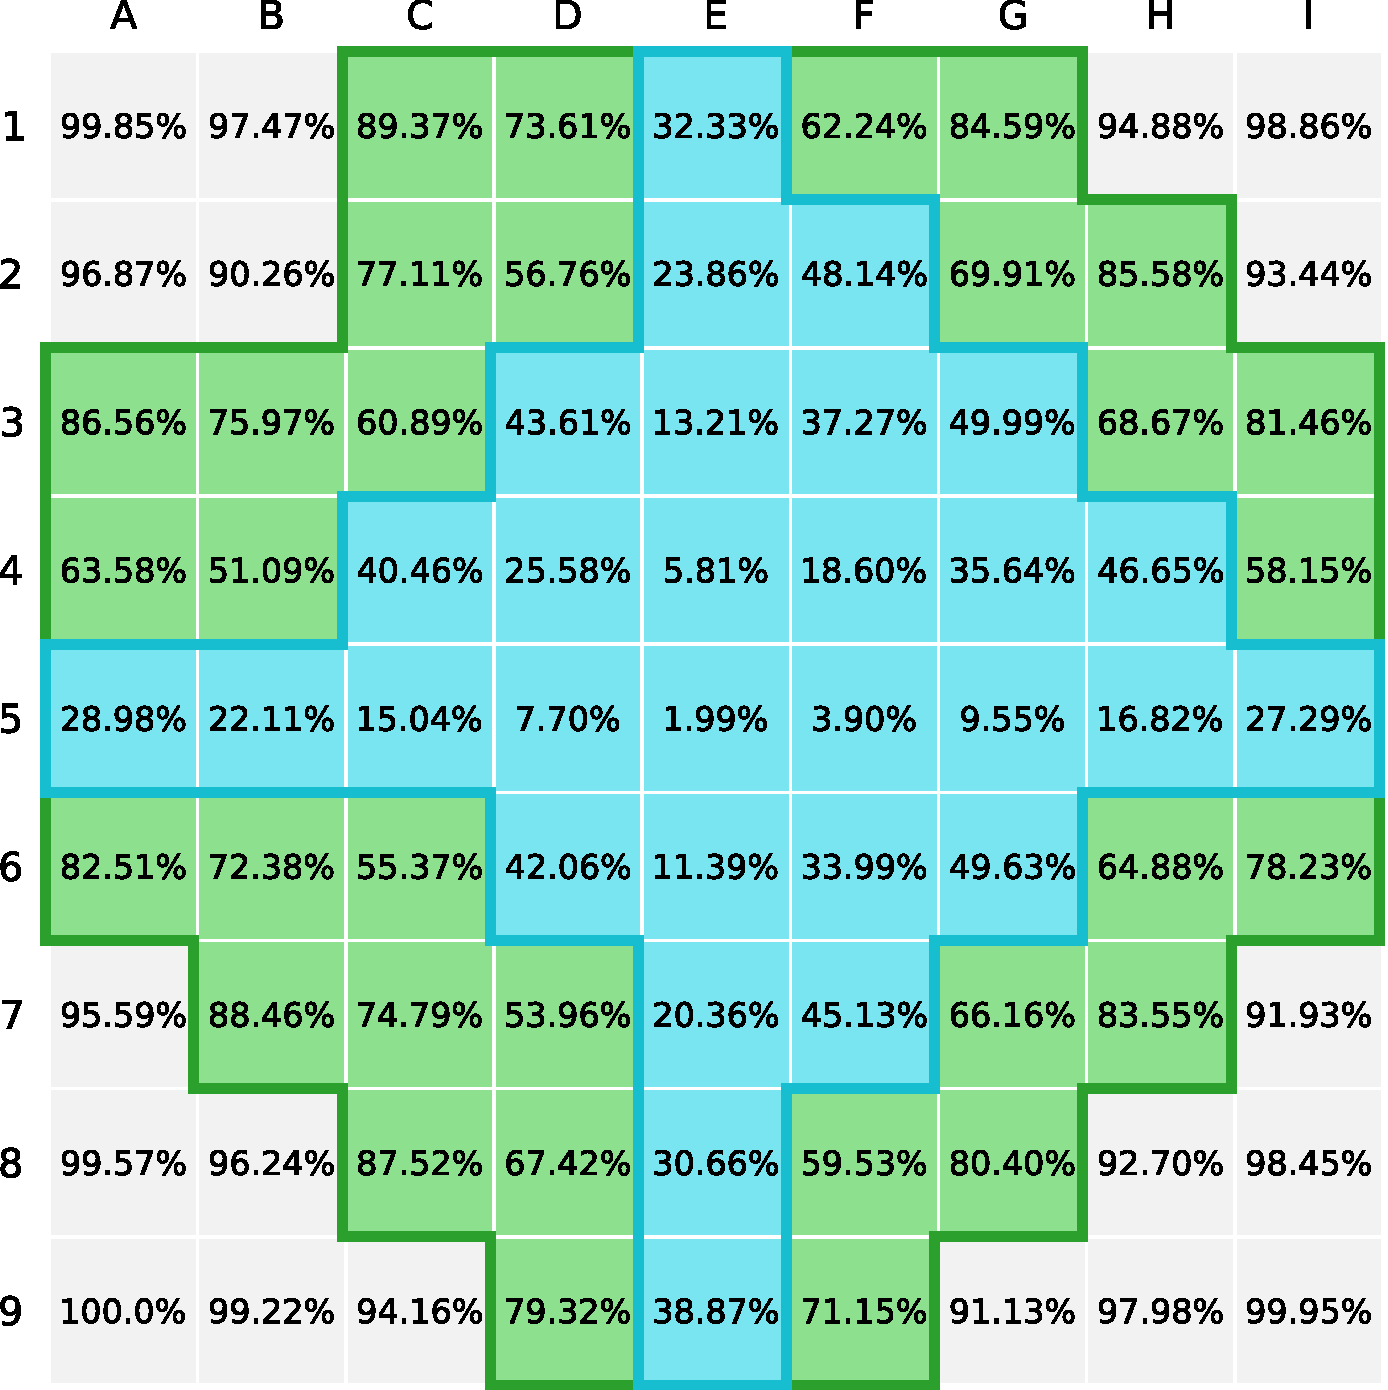
\includegraphics[width=0.95\linewidth]{images/sim/sim_skymap_conts.pdf}

\end{center}

\caption[An example 2D skymap with pixel contour values]{The same cartoon skymap as in \aref{fig:sim_skymap_probs}, but now each pixel contains its contour value. These are calculated by sorting the pixels by probability and assigning each the value of the cumulative sum. The pixel with the highest probability (E5) has the same contour value as its probability value, the second highest (F5) has the sum of the probability values of both E5 and F5, and this continues to the pixel with the lowest probability value (A9) which has a contour value of 100\%. The thick blue line is the 50\% probability contour, which encloses all pixels with a contour value of less than 50\%. The green line likewise encloses all pixels with a contour value of less than 90\%.
}
\label{fig:sim_skymap_conts}
\end{figure}

% -----

\end{colsection}

% ~~~~~~~~~~~~~~~~~~~~

\subsection{Mapping skymaps to grids}
\label{sec:mapping_skymaps}
\begin{colsection}

When gravitational wave signals are detected the \gls{lvc} analysis pipelines create HEALPix skymaps to describe the sky localisation, and these are then distributed with the public VOEvent (see \aref{sec:voevents}). GOTO-tile is used to map the skymaps onto the previously-defined sky grid used for the all-sky survey. This requires finding which HEALPix pixels fall within each tile, which is done by defining polygons that match the projected tile areas and using the \pkg{healpy} \code{query\_polygon} function. Then it is simple to sum the probability of these pixels for each tile to give the total probability contained within it. As sky grids might contain overlapping tiles a given pixel may fall within multiple tiles, and therefore contribute to the total probability of more than one tile.

Finding which contour each tile is in is not as simple, and there are multiple ways to define the contour value for the tiles. \aref{fig:sim_skymap_tiles} shows calculating the contained probabilities for tiles using the previous 2D skymap, as well as two methods to calculate the contour values: taking the minimum or the mean of the contained pixel contour values. Using the mean is preferred as it is less susceptible to single outlier pixels.

% -----

\begin{figure}[p]

\begin{center}
\begin{tabular}{cccccc}
\multicolumn{3}{c}{Pixel probabilities (from \aref{fig:sim_skymap_probs}):} &
\multicolumn{3}{c}{Pixel contours (from \aref{fig:sim_skymap_conts}):}
\\
\multicolumn{3}{c}{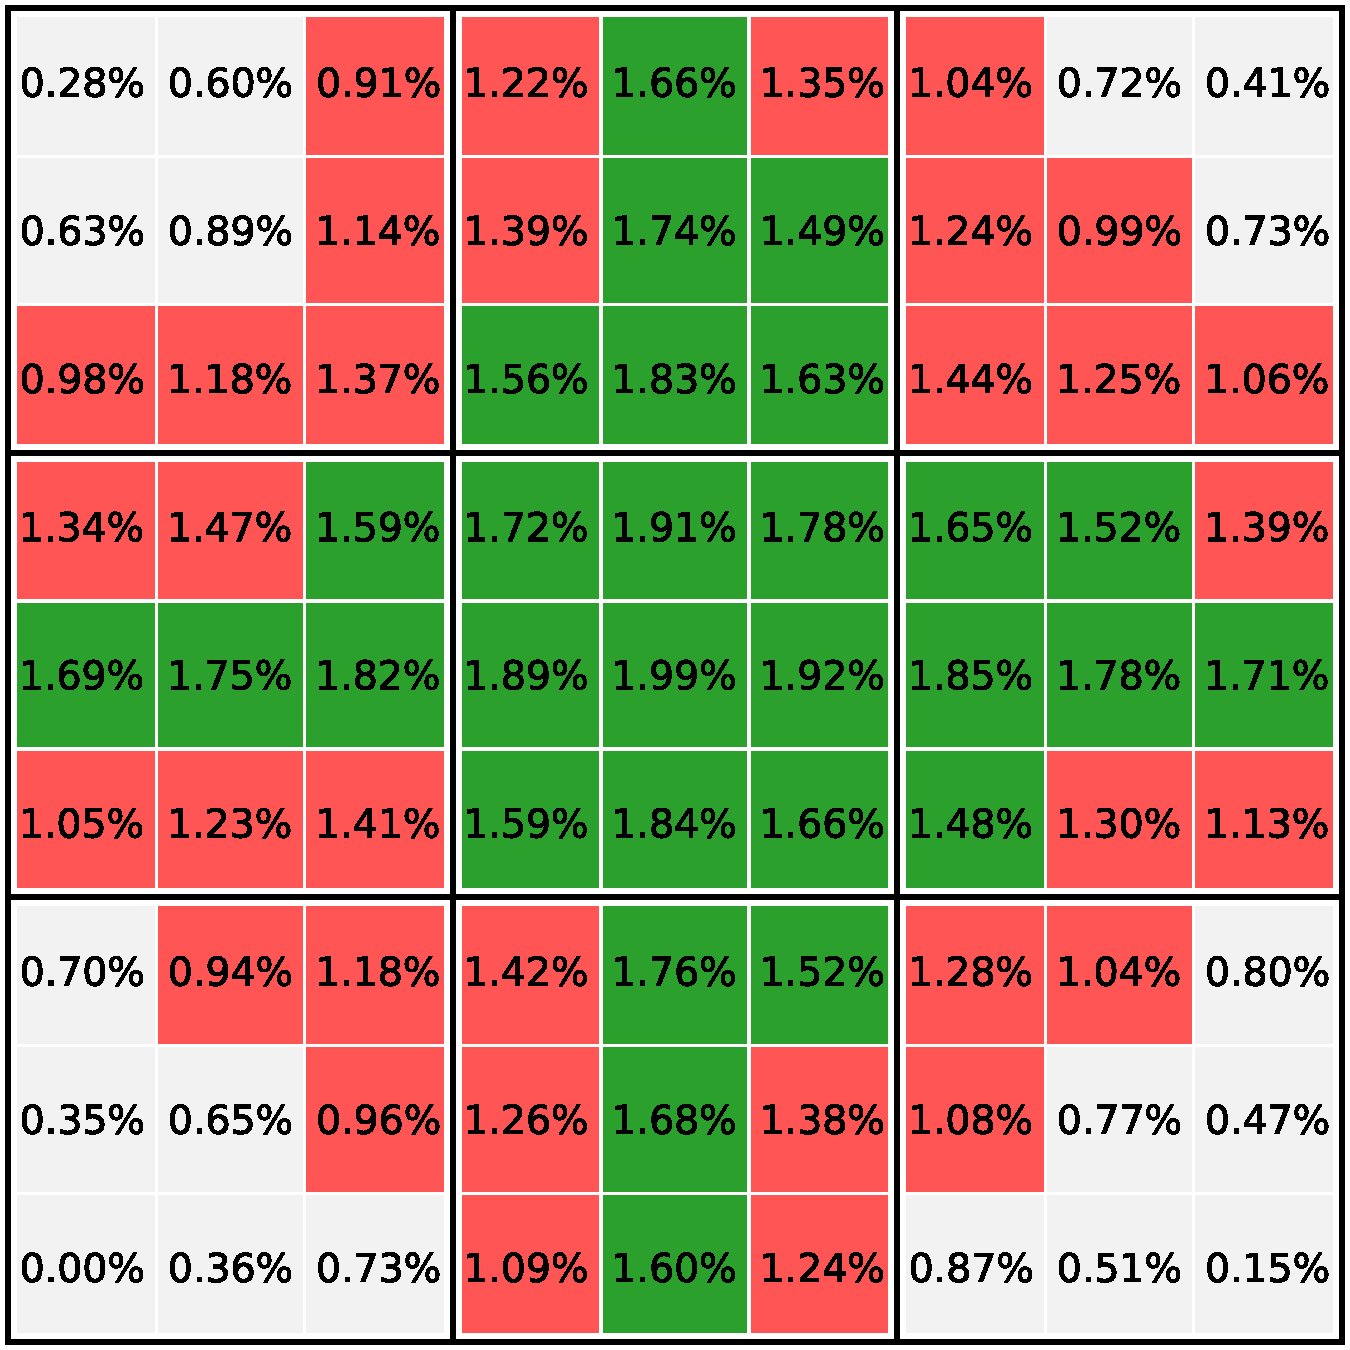
\includegraphics[width=0.46\linewidth]{images/sim/sim_skymap_pix_probs.pdf}} &
\multicolumn{3}{c}{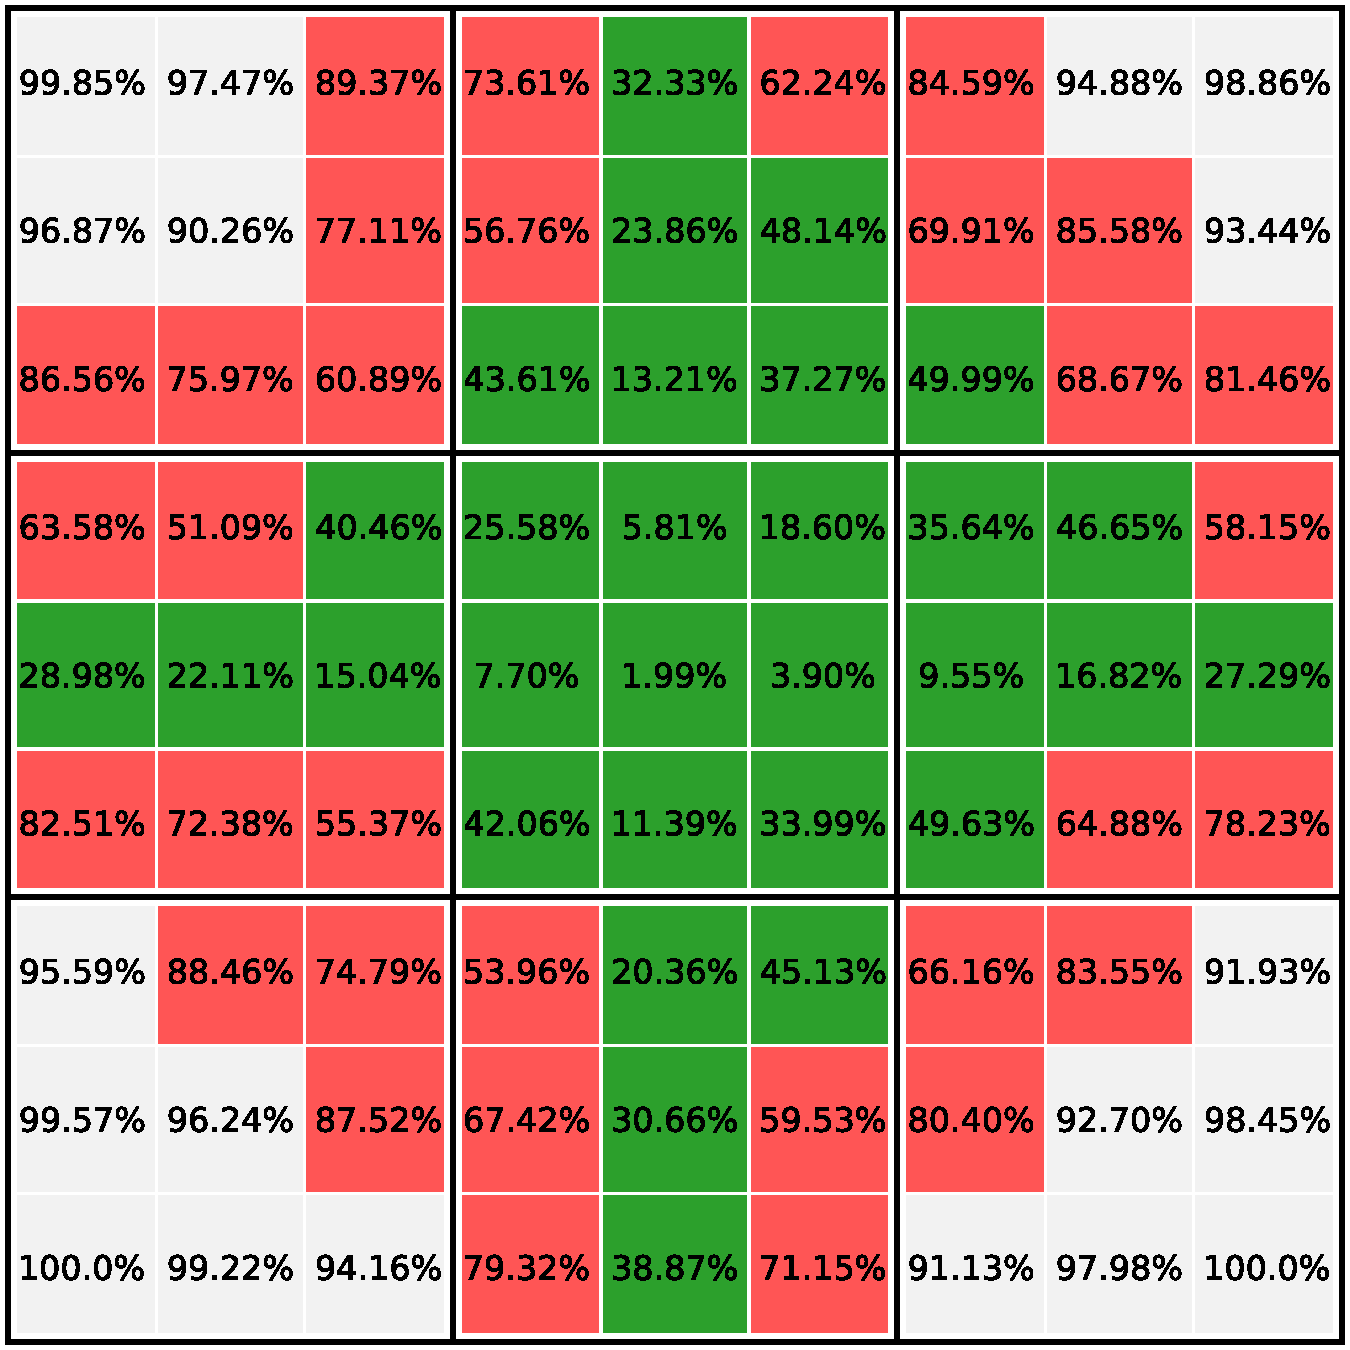
\includegraphics[width=0.46\linewidth]{images/sim/sim_skymap_pix_conts.pdf}}
\\
\multicolumn{2}{c}{Tile contained probabilities:} &
\multicolumn{2}{c}{Tile minimum contours:} &
\multicolumn{2}{c}{Tile mean contours:}
\\
\multicolumn{2}{c}{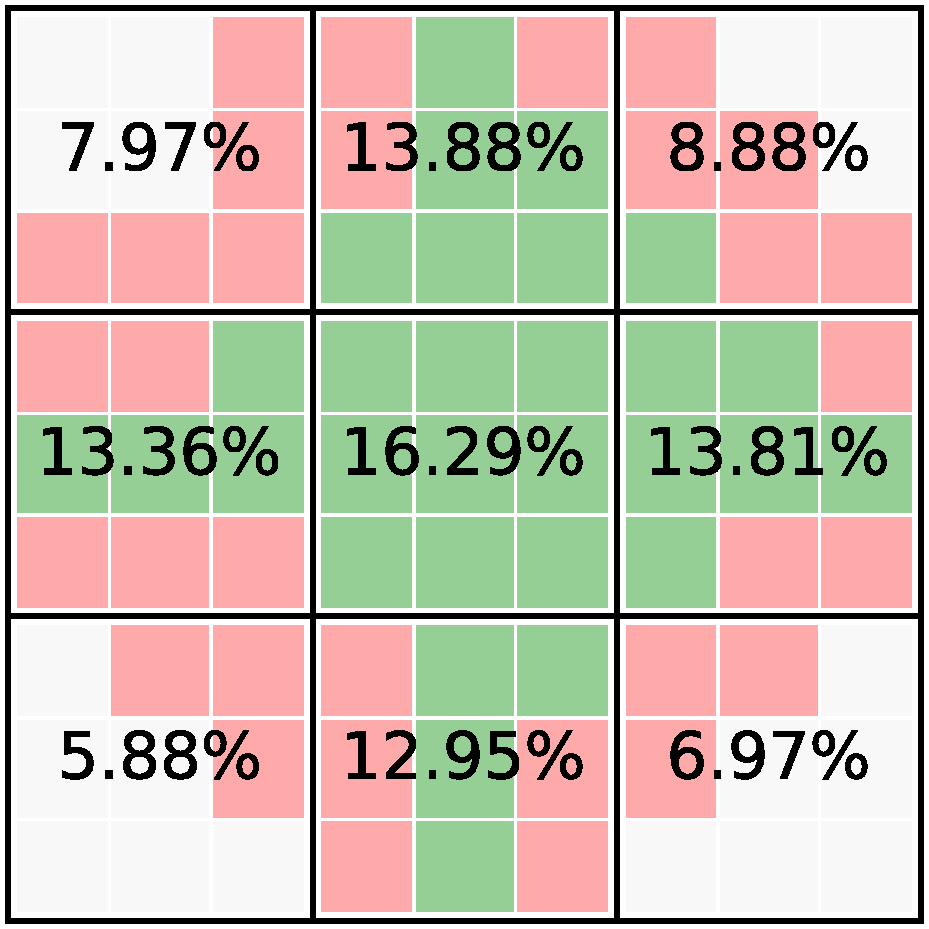
\includegraphics[width=0.3\linewidth]{images/sim/sim_skymap_tile_probs.pdf}} &
\multicolumn{2}{c}{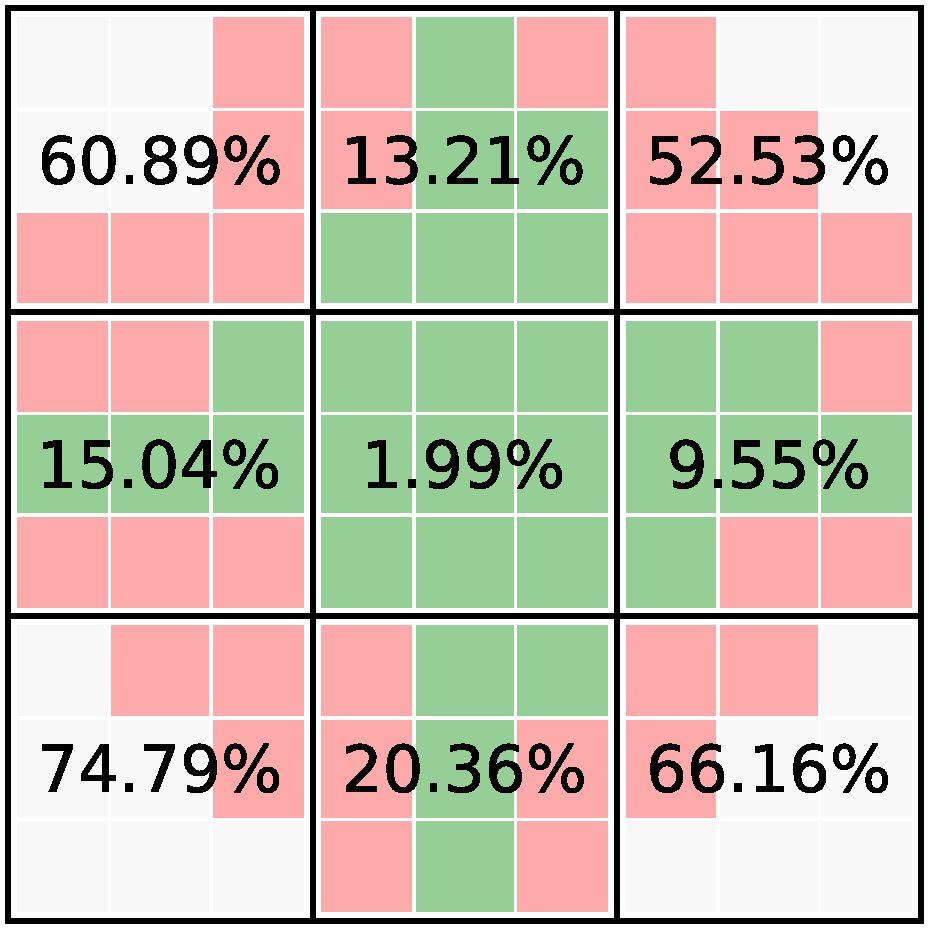
\includegraphics[width=0.3\linewidth]{images/sim/sim_skymap_tile_minconts.pdf}} &
\multicolumn{2}{c}{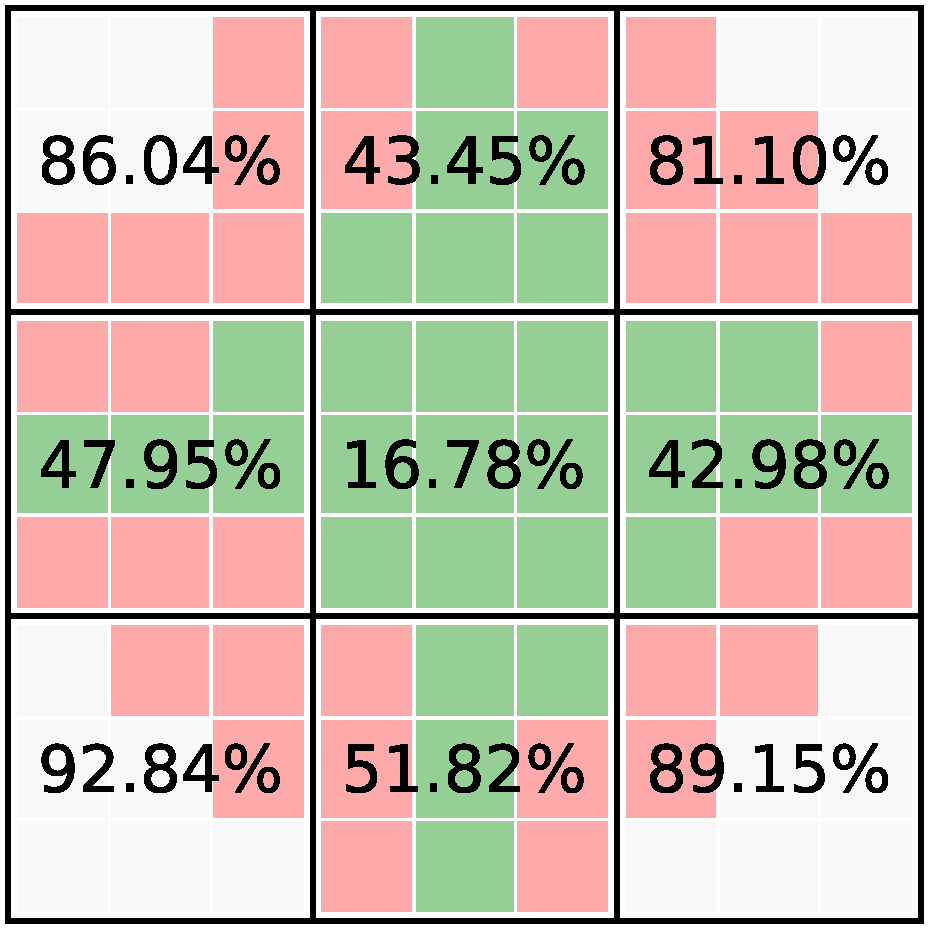
\includegraphics[width=0.3\linewidth]{images/sim/sim_skymap_tile_meanconts.pdf}}
\\
\end{tabular}
\end{center}

\caption[Calculating tile probabilities and contours for a 2D skymap]{Tiling the same cartoon 2D skymap as \aref{fig:sim_skymap_probs} and \aref{fig:sim_skymap_conts}.\\
\textbf{Top}: These plots show the pixel probabilities and contour values, coloured with the pixels within the 50\% contour in green and the pixels within the 90\% contour in green or red. The 81 total pixels are divided into 9 tiles, with no overlap for simplicity.\\
\textbf{Lower-right}: The contained probability within each tile is the sum of the pixel probabilities, in this case each tile contains the sum of the 9 pixels contained within. Overlapping tiles would mean a single pixel might fall within multiple tiles and therefore contribute probability to each.\\
\textbf{Lower-centre}: One way of finding which contour area each tile is within is to find the minimum contour value of the 9 pixels contained within it. This corresponds to the contour value of the pixel with the highest probability within each tile.\\
\textbf{Lower-right:} An alternative method is to calculate the mean contour value of the pixels within each tile and use that as the tile contour value. This is less susceptible to single pixels affecting the value than taking the minimum.
}
\label{fig:sim_skymap_tiles}
\end{figure}

% -----

\clearpage

\aref{fig:170817_gw} shows an example of GOTO-tile applied to the skymap for the GW170817 event \citep{GW170817}. The points within each tile were identified and summed in order to find the total contained probability within each tile. There is some redundancy due to the overlap between tiles, however this is typically negligible (the final GW170817 skymap used was notably smaller than usual LVC skymaps due to the coincident \textit{Fermi} localisation, which makes the overlaps more pronounced).

\begin{figure}[p]
\begin{center}
\includegraphics[width=\linewidth]{images/skymaps_170817_gw.pdf}
\end{center}
\caption[Tile probabilities for GW170817]{Tile probabilities using the final skymap for GW170817 \citep{GW170817}. The sphere shows the whole skymap for this event, with each pixel coloured by probability, and the location of the source of the event is shown with the blue star. Overlaid is the GOTO-4 sky grid, with tiles of \SI{3.7}{\degree} $\times$ \SI{4.9}{\degree} and overlap of $0.1$. The inset shows the tiles coloured by their contained probability (the sum of all pixels within). The four tiles with contained probability of higher than 5\% are highlighted in red.
}
\label{fig:170817_gw}
\end{figure}

\clearpage

\end{colsection}

% ~~~~~~~~~~~~~~~~~~~~

\subsection{Creating skymaps for GRB events}
\label{sec:gaussian_skymaps}
\begin{colsection}

This system described in the previous sections works well for gravitational wave events using \gls{lvc} skymaps, and it has since ben expanded to other types of events. As part of the commissioning observations (\rtxt{see commissioning}) when the LIGO-Virgo detectors were down \gls{goto} also followed-up \gls{grb} events from the \textit{Fermi} satellite \gls{gbm} \citep{Fermi_GBM}. These events however do not include probability skymaps, instead they only include a central right ascension, declination and error radius. Yik Lun Mong and I developed code in order to create a skymap from these Fermi events, therefore allowing them to be processed by GOTO-tile using the same methods already created for gravitational wave events.

Instead of loading a skymap from a FITS file, a function was written to create a probability skymap based on a 2D Gaussian profile. First, the error radius ($r$, the 68\% containment radius) is converted into the standard deviation of the distribution $\sigma$ using

\begin{equation}
    \sigma = \frac{r}{\sqrt{2.3}}.
    \label{eq:gaussian_sigma}
\end{equation}

The distance $d$ between a given point on the sphere ($\alpha, \delta$) and the central coordinates of the distribution ($\alpha_c, \delta_c$) is given by

\begin{equation}
    \sin^2 \left ( \frac{1}{2} d \right )
    = \sin^2 \left ( \frac{\delta-\delta_c}{2} \right)
      + \cos (\delta) \cos (\delta_c) \sin^2 \left ( \frac{\alpha-\alpha_c}{2} \right),
    \label{eq:gaussian_distance}
\end{equation}

and the probability at each point is given by

\begin{equation}
    P(\alpha, \delta) = \frac{1}{2\pi\sigma} \exp \left ( \frac{d^2}{2\sigma^2} \right ).
    \label{eq:gaussian_prob}
\end{equation}

In order to create a HEALPix skymap this probability is calculated for every point on the grid, which creates the skymap array. This can then be processed with GOTO-tile exactly like an \gls{lvc} skymap.

Using this above method, skymaps can be created for any single-target alert that has a given error radius. Several sources of transient events, such as \textit{Gaia} or \textit{Swift}, produce very well-localised events with error regions well below the field of view of GOTO, so creating skymaps is less important. The skymaps for \glspl{grb} from \textit{Fermi} however cover much larger areas. For example, the \gls{gbm} detection of GRB~170817A that helped localise the GW170817 gravitational wave detection produced an initial alert with an error radius of \SI{17.45}{\degree}, later reduced to \SI{11.58}{\degree} in the final alert\footnote{GCN Notices available at \url{https://gcn.gsfc.nasa.gov/other/524666471.fermi}}, which corresponded to a 50\% confidence region of $\sim$500~square~degrees \citep{GW170817_Fermi}. The error values given in \gls{gbm} GCN Notices however only account for statistical errors for that event, not systematic errors. The \gls{gbm} systematic errors are described in \citet{Fermi_localisation} to be well modelled by a core Gaussian with a radius of \SI{3.71}{\degree} and a non-Gaussian tail extending to \SI{14}{\degree}. For the purposes of \gls{goto} tiling the tail is ignored, and a single Gaussian is produced with an error radius simply combining the statistical radius ($r_\text{notice}$) and this  systematic profile in quadrature as

\begin{equation}
    r = \sqrt{r_\text{notice}^2 + {(\SI{3.71}{\degree})}^2}.
    \label{eq:fermi_radius}
\end{equation}

This radius is then used with \aref{eq:gaussian_sigma} onwards to create the Gaussian skymap. It should be noted that in reality the probability areas from \textit{Fermi} are not perfectly symmetric Gaussian profiles, but until \gls{gbm} events start being published with \gls{healpix} skymaps this works as a reasonable approximation. For GRB~170817A the skymap and tiling solution is shown in \aref{fig:170817_grb}. Note that the source location falls quite far out of the peak of the \gls{grb} skymap, and had there not been the coincident gravitational wave detection it would be unlikely that the source of the gamma-ray burst would have been observed.

\begin{figure}[p]
\begin{center}
\includegraphics[width=\linewidth]{images/skymaps_170817_grb.pdf}
\end{center}
\caption[Tile probabilities for GRB 170817A]{Tile probabilities using the constructed Gaussian skymap for GRB 170817A \citep{GW170817_Fermi}. As in \aref{fig:170817_gw} the sphere shows the skymap and the GOTO-4 grid, with the identified source of GW170817 shown by the blue star. The tiles highlighted in red each contain more than 1\% of the probability instead of 5\% used in \aref{fig:170817_gw}, due to the greater spread of the skymap meaning no tile here contains more than 5\%.
}
\label{fig:170817_grb}
\end{figure}

\end{colsection}

% ~~~~~~~~~~~~~~~~~~~~

\end{colsection}

% ########################################

\newpage
\section{Alert processing with GOTO-alert}
\label{sec:gotoalert}
\begin{colsection}

% ~~~~~~~~~~~~~~~~~~~~

\begin{colsection}

GOTO-alert is another \proglang{Python} module (\pkg{gotoalert} \rtxt{footnote url?}) created for the \gls{goto} project to contain functions related to alert handling and VOEvents. It was originally created based on code written by Alex Obradovic (a student at Monash) for \gls{grb} events. After he uploaded his code I reworked it into an object-oriented Python module and integrated it into the wider \gls{goto} software ecosystem, specifically adding in functions related to the GOTO-tile and ObsDB modules as well as creating a more advanced strategy system.

\end{colsection}

% ~~~~~~~~~~~~~~~~~~~~

\subsection{GCN alerts}
\label{sec:gcn}
\begin{colsection}

The \gls{gcn}, also known as the Transient Astronomy Network or together GCN/TAN, is a system hosted by NASA originally to publish alerts relating to gamma-ray burst detections \citep{GCN}. It publishes events from a variety of telescopes including \textit{INTEGRAL}, \textit{Fermi} and \textit{Swift}, and more recently has expanded to neutrino and gravitational wave alerts --- including publishing alerts from the LIGO-Virgo Collaboration.

Alerts are produced by the projects and missions in the form of \gls{gcn} Notices, standard machine-readable text messages that are distributed by the network. Notices are designed to be written and sent out automatically by the instrument without the need for human intervention, and likewise can be received and acted on by automated systems run by follow-up projects such as \gls{goto}'s sentinel. Transmitting notices is only done by the projects that are part of the network.

There is a second form of alerts distributed by the network called \gls{gcn} Circulars. Unlike notices, circulars are designed to be written by humans and sent out by email to anyone subscribed to the distribution list. They act as a formal, citable way to share information about events: both the detection by the instrument but also follow-up activity from other groups.

\end{colsection}

% ~~~~~~~~~~~~~~~~~~~~

\subsection{VOEvents}
\label{sec:voevents}
\begin{colsection}

The GCN/TAN system broadcasts notices in multiple ways over many different channels, but the most useful for automated telescopes such as \gls{goto} uses the \gls{ivoa} VOEvent standard \citep{voevent}. VOEvents are a standard way to transmit information about transient astronomical events, in a structured format to make the reports easily machine-readable. Each event is assigned an \gls{ivorn} and follows a defined schema. By defining a standard template to follow diverse events can all be universally processed and robotic telescopes triggered without the need for human interpretation or vetting.

The structure to transmit these events is fairly flexible, but there are certain common roles. The names below are taken from \citet{voevent}:

\begin{itemize}
    \item \textbf{Authors} are the projects, instruments or institutions that create the original data worthy of reporting in the VOEvent.
    \item \textbf{Publishers} take the information about the astronomical event, put it into the VOEvent format and broadcast it from their servers.
    \item \textbf{Brokers} act as nodes in the communication web, they can take in events from multiple publishers and rebroadcast them in a single stream.
    \item \textbf{Subscribers} are the end users that listen to VOEvent servers (either directly to the publishers or a common broker).
\end{itemize}

In some cases roles can be combined, but for the case of \gls{goto} receiving \gls{lvc} events there are distinct actors: the LIGO-Virgo Collaboration is the author, NASA and the GCN/TAN system are the publishers and the \gls{goto} sentinel is the subscriber.

It is possible to listen directly to the GCN/TAN servers, in which case the sentinel would receive VOEvents from the NASA missions and other projects like \gls{ligo}. However there are other groups out there publishing their own VOEvents separate to the GCN system which we might want to receive. It would be possible to run multiple event listeners within the sentinel, each listening to other servers, but it is much easier to listen to a common broker that already does that and provides a single point of access to these pipelines. The broker chosen for the \gls{gtecs} sentinel is the same as for pt5m: the 4 Pi Sky VOEvents Hub \citep{4pisky}.

4 Pi Sky provides alerts from the GCN system\footnote{\url{https://gcn.gsfc.nasa.gov/burst_info.html}} as well as from the Gaia\footnote{\url{http://gsaweb.ast.cam.ac.uk/alerts/alertsindex}} and \gls{asassn}\footnote{\url{http://www.astronomy.ohio-state.edu/~assassin/transients}} projects. At the time of writing \gls{goto} only follows up \gls{lvc} \gls{gw} as well as \textit{Fermi} and \textit{Swift} \gls{grb} events, all of which are published through \glspl{gcn}, meaning there's technically no benefit of listening to 4 Pi Sky over listening directly to NASA.\@ However pt5m automatically followed up Gaia events meaning the 4 Pi Sky broker was necessary, and it has been suggested \gls{goto} could do the same.

In order to receive VOEvents from any source it is necessary to set up a VOEvent client. The most common way to do this is using the \software{Comet} software \citep{comet}, which allows both sending and receiving of events. For the \gls{gtecs} sentinel (see \aref{sec:sentinel}) all that was needed was a simple way to listen to and download alerts, which is why it instead uses code based on the \software{Python} module PyGCN (\pkg{pygcn}\footnote{\url{https://github.com/lpsinger/pygcn}}). Despite the name, PyGCN works perfectly fine to receive any VOEvents, not just those from the GCN servers. The sentinel uses PyGCN to open a socket to the 4 Pi Sky server and ingest binary packets, as well as sending the required receipt and ``\code{iamalive}'' responses to the server to ensure it keeps receiving events.

VOEvents take the form of a structured \gls{xml} document. \gls{xml} is a ``markup'' language similar to HTML, JSON or \LaTeX, meaning it is understandable by humans but follows a set schema and so can be easily read and processed by computers. A sample of a VOEvent is given in \aref{fig:voevent_xml}.

\begin{figure}[p]
\begin{lstlisting}[language=xml,
       tabsize=2,
       breaklines=true,
       keywordstyle={},
       stringstyle=\color{red},
       showstringspaces=false,
       basicstyle=\scriptsize,
       emph={voe,Who,What,WhereWhen,How,Citations},
       emphstyle={\color{magenta}}
       ]
<?xml version=\'1.0\'
      encoding=\'UTF-8\'?>\n<voe:VOEvent
      xmlns:xsi="http://www.w3.org/2001/XMLSchema-instance"
      xmlns:voe="http://www.ivoa.net/xml/VOEvent/v2.0"
      xsi:schemaLocation="http://www.ivoa.net/xml/VOEvent/v2.0
                          http://www.ivoa.net/xml/VOEvent/VOEvent-v2.0.xsd"
      role="observation"
      ivorn="ivo://gwnet/LVC#S190408an-2-Initial">
<Who>
 <Date>2019-04-08T20:21:42</Date>
 <Author>
  <contactName>LIGO Scientific Collaboration and Virgo Collaboration</contactName>
 </Author>
</Who>
<What>
 <Param name="Packet_Type" dataType="int" value="151"></Param>
 <Param name="internal" dataType="int" value="0"></Param>
 <Param name="Pkt_Ser_Num" dataType="string" value="2"></Param>
 <Param name="GraceID" dataType="string" value="S190408an" ucd="meta.id"></Param>
 <Param name="AlertType" dataType="string" value="Initial" ucd="meta.version"></Param>
 <Param name="HardwareInj" dataType="int" value="0" ucd="meta.number"></Param>
 <Param name="OpenAlert" dataType="int" value="1" ucd="meta.number"></Param>
 <Param name="EventPage" dataType="string" value="https://gracedb.ligo.org/superevents/S190408an/view/" ucd="meta.ref.url"></Param>
 <Param name="Instruments" dataType="string" value="H1,L1,V1" ucd="meta.code"> </Param>
 <Param name="FAR" dataType="float" value="2.81096164616e-18" ucd="arith.rate;stat.falsealarm" unit="Hz"></Param>
 <Param name="Group" dataType="string" value="CBC" ucd="meta.code"></Param>
 <Param name="Pipeline" dataType="string" value="gstlal" ucd="meta.code"></Param>
 <Param name="Search" dataType="string" value="AllSky" ucd="meta.code"></Param>
 <Group type="GW_SKYMAP" name="bayestar">
  <Param name="skymap_fits" dataType="string" value="https://gracedb.ligo.org/api/superevents/S190408an/files/bayestar.fits.gz" ucd="meta.ref.url"></Param>
 </Group>
 <Group type="Classification">
  <Param name="BNS" dataType="float" value="0.0" ucd="stat.probability"></Param>
  <Param name="NSBH" dataType="float" value="0.0" ucd="stat.probability"></Param>
  <Param name="BBH" dataType="float" value="0.99999999999" ucd="stat.probability"></Param>
  <Param name="MassGap" dataType="float" value="0.0" ucd="stat.probability"></Param>
  <Param name="Terrestrial" dataType="float" value="9.82357724531e-12" ucd="stat.probability"></Param>
 </Group>
 <Group type="Properties">
  <Param name="HasNS" dataType="float" value="0.0" ucd="stat.probability"></Param>
  <Param name="HasRemnant" dataType="float" value="0.12" ucd="stat.probability"></Param>
 </Group>
</What>
<WhereWhen>
 <ObsDataLocation>
 <ObservatoryLocation id="LIGO Virgo"/>
 <ObservationLocation>
 <AstroCoordSystem id="UTC-FK5-GEO"/>
 <AstroCoords coord_system_id="UTC-FK5-GEO">
 <Time><TimeInstant><ISOTime>2019-04-08T18:18:02.288180</ISOTime></TimeInstant></Time>
 </AstroCoords>
 </ObservationLocation>
 </ObsDataLocation>
</WhereWhen>
...
\end{lstlisting}
\caption[VOEvent XML sample]{A sample of VOEvent \gls{xml} text from an \gls{lvc} event, formatted so the core \gls{xml} structure is visible. Some of the key pieces of information are the role and \gls{ivorn} defined in the header, the URL of the skymap and the event classification probabilities.
}
\label{fig:voevent_xml}
\end{figure}

\newpage

\end{colsection}

% ~~~~~~~~~~~~~~~~~~~~

\subsection{Event handling}
\label{sec:event_handling}
\begin{colsection}

Once the VOEvent is received by the \gls{gtecs} sentinel the work of parsing and processing the event uses another \proglang{Python} module GOTO-Alert (\pkg{gotoalert}).

% ---------
\subsubsection{Event classes}

At the core of the GOTO-alert code is the \code{Event} object class. An Event is created from a raw binary payload from the PyGCN VOEvent client, and from the \gls{xml} a \proglang{Python} class is populated with the basic event information (\gls{ivorn}, type, source etc). Once the basic Event is created it is checked against an internal list of so-called ``interesting'' event packet types --- the ones we care about processing for \gls{goto}. At the time of writing these are \code{SWIFT\_BAT}, \code{FERMI\_GBM} and \code{LVC} events, as listed in \aref{tab:events}. If the event matches any of the recognised packet types then the Event is subclassed into a new object, which allows more specific properties and methods. The current classes are as follows:

\begin{itemize}
    \item \code{GRBEvent} is the class used for events relating to a Gamma-Ray Bust detections, specifically from \textit{Fermi} and \textit{Swift}. The VOEvents for these events contain a sky position in right ascension and declination as well as an error radius, so a HEALPix skymap is produced using the Gaussian method described in \aref{sec:gaussian_skymaps}. For \textit{Fermi} events the class also has an additional attribute extracted from the VOEvent: the \textbf{duration} of the burst (Long or Short). This property could then be used to select different observing strategies for either type of burst.

    \item \code{GWEvent} is the class used for \gls{lvc} gravitational wave events, for all three \gls{lvc} detection notice types (``Preliminary'', ``Initial'' and ``Update''). As these are events produced by LIGO-Virgo they should contain a \code{skymap\_fits} parameter which gives a URL for where the skymap can be downloaded from GraceDB, the \gls{ligo} event database (as shown in \aref{fig:voevent_xml}). The gravitational wave VOEvents also contain a variety of properties that are stored on the event class and which can be used to decide which observing strategy to use \citep{LVC_userguide}. These include:
    \begin{itemize}
        \item \textbf{\gls{far}}: a value provided to contain the estimated probability that this event is a false alarm i.e.\ not from a real astronomical source. Given in the form of an expected frequency or rate, so an event with a false alarm rate of 1 per year is much more tenuous than one with a \gls{far} of 1 per 10,000 years.
        \item \textbf{Instruments}: which of the three \gls{lvc} \gls{gw} instruments (\gls{ligo}-Livingston, \gls{ligo}-Hanford and Virgo) detected the signal. Non-detection in one or more instruments is accounted for in the \gls{far}.
        \item \textbf{Group}: which type of pipeline detected the event signal, either ``\gls{cbc}'' or ``Burst''. The following parameters only apply to \gls{cbc} events.
        \item \textbf{Classification}: the VOEvents for \gls{cbc} events contain probabilities that the source falls into one of five categories: \gls{bns} merger, \gls{nsbh} merger, \gls{bbh} merger, ``MassGap'' merger (one or other of the components is in the hypothetical ``mass gap'' between neutron stars and black holes, defined as 3--\SI{5}{\solarmass} \citep{GW_MassGap}) or ``Terrestrial'' (a non-astronomical source).
        \item \textbf{Properties}: \gls{cbc} events also contain two important properties: ``HasNS'', the probability one or both of components is consistent with a neutron star ($<$\SI{3}{\solarmass}), and ``HasRemnant'', the modelled probability a non-zero amount of material was ejected during coalescence and therefore an electromagnetic signal might be expected.
        \item \textbf{Distance}: The skymaps produced by the \gls{lvc} contain full three-dimensional localisation information \citep{GW_distance}. For deciding on event strategy only the mean distance is stored from the skymap \gls{fits} header, in megaparsec, along with the standard deviation.
    \end{itemize}

    \item \code{GWRetractionEvent} is a special Event subclass to deal with \gls{lvc} notices that are retractions of earlier events. They are effectively just a more limited version of the \code{GWEvent} class as they don't contain a skymap or any of the additional parameters listed above. Having retraction events occupy their own subclass makes it easier to identify and process them when sent through the event handler.

\end{itemize}

\begin{table}[t]
\begin{center}
\begin{tabular}{clll}

Packet type & Source              & Notice type                  & Event subclass           \\
\midrule
\code{61}   & NASA/\textit{Swift} & \code{SWIFT\_BAT\_GRB\_POS}  & \code{GRBEvent}          \\
\code{115}  & NASA/\textit{Fermi} & \code{FERMI\_GBM\_FIN\_POS}  & \code{GRBEvent}          \\
\code{150}  & \gls{lvc}           & \code{LVC\_PRELIMINARY}      & \code{GWEvent}           \\
\code{151}  & \gls{lvc}           & \code{LVC\_INITIAL}          & \code{GWEvent}           \\
\code{152}  & \gls{lvc}           & \code{LVC\_UPDATE}           & \code{GWEvent}           \\
\code{164}  & \gls{lvc}           & \code{LVC\_RETRACTION}       & \code{GWRetractionEvent} \\

\end{tabular}
\end{center}
\caption[GCN notices recognised by the GOTO-alert event handler]{GCN notices and corresponding classes recognised by the GOTO-alert event handler.}
\label{tab:events}
\end{table}

% ---------
\subsubsection{The event handler}

Once the correct Event class has been created the sentinel passes it to the GOTO-alert \code{event\_handler} function. Before processing the event the handler first has to filter out any uninteresting events, where ``interesting'' events are defined as those that fall into any of the above subclasses. If the event passed to the function is not one of those then it is rejected and the handler exits at this point. The handler will also reject an Event that is ``interesting'' if it has an incorrect role. \gls{lvc} sends out test VOEvents to allow full testing of any follow-up systems, these are identical to real events (even including simulated skymaps) but are explicitly marked as \code{test} events in their role. These can be optionally processed by the event handler, but in the live sentinel system they are also rejected at this point.

If the event passes the above filter the next step is to download the event's skymap (for \gls{gw} events) or create a corresponding Gaussian skymap (for \gls{grb} events). Doing this after filtering out uninteresting events saves time and processing power downloading or creating skymaps that aren't used, for example for \gls{lvc} test events.

Once the event has an associated skymap the observing strategy for the event can be generated. This can only happen after the skymap is downloaded as some parameters, notably the distance for \gls{gw} events, are only stored within the skymap headers instead of in the VOEvent \gls{xml}. The details of the different event strategies and how they are defined are given in \aref{sec:event_strategy}.

Finally the event handler inserts pointings and other information into the observation database, with parameters depending on the strategy determined in the previous stage. This is detailed in \aref{sec:db_insert}.

% ---------
\subsubsection{\software{Slack} alerts}

Throughout the event handling process GOTO-alert has the option of sending confirmation messages to Slack, in a similar way to the \gls{gtecs} pilot (see \aref{fig:pilot_slack}). This allows human observers to be informed of any new alerts processed by the sentinel, as well as the expected outcome of upcoming observations. The function deliberately spaces out the alerts it sends at different stages within the code, rather than sending them all at the end, to make sure it's obvious if a problem occurs and one or more alerts are missing. Four alerts are sent out in total:

\begin{enumerate}
    \item An initial alert is sent out by the sentinel as soon as an interesting event is received, and contains only one line reporting the IVORN of the event to be processed. Sending this first means there is a record should an error occur subsequently while handling the event.
    \item The first alert is sent out by GOTO-alert once the event has been created and the skymap downloaded. It contains the key information and properties of the event, as well as a plot of the event skymap produced by GOTO-tile.
    \item The next alert is sent out after the event observing strategy has been retrieved, and reports the contents of the strategy dictionaries (see \aref{sec:event_strategy}).
    \item The final alert is sent out after the event tiles have been added to the observation database (see \aref{sec:db_insert}). As well as showing the number of tiles selected and their combined skymap coverage this alert also contains predictions of which tiles will be visible from the GOTO site in La Palma over the valid period. Ultimately this could also include a second corresponding calculation of visibility from GOTO-South as well. Note this is only a rough prediction based on visible altitudes during the night, and therefore excluding weather conditions, the position of the Moon and the existence of any higher-priority pointings that would take precedence (see \aref{sec:scheduler} for how the \gls{gtecs} just-in-time scheduler operates).
\end{enumerate}

The three detailed alerts generated by GOTO-alert for an example \gls{gw} event are shown in \aref{fig:pilot_slack}.

Should a retraction notice be received for an event previously processed by the sentinel then strategy and visibility alerts would not be applicable. Instead once it has been handled a special alert will be sent out, clarifying that the retraction was received and any previously-inserted pointings have been deleted.

\begin{sidewaysfigure}[p]
\begin{center}
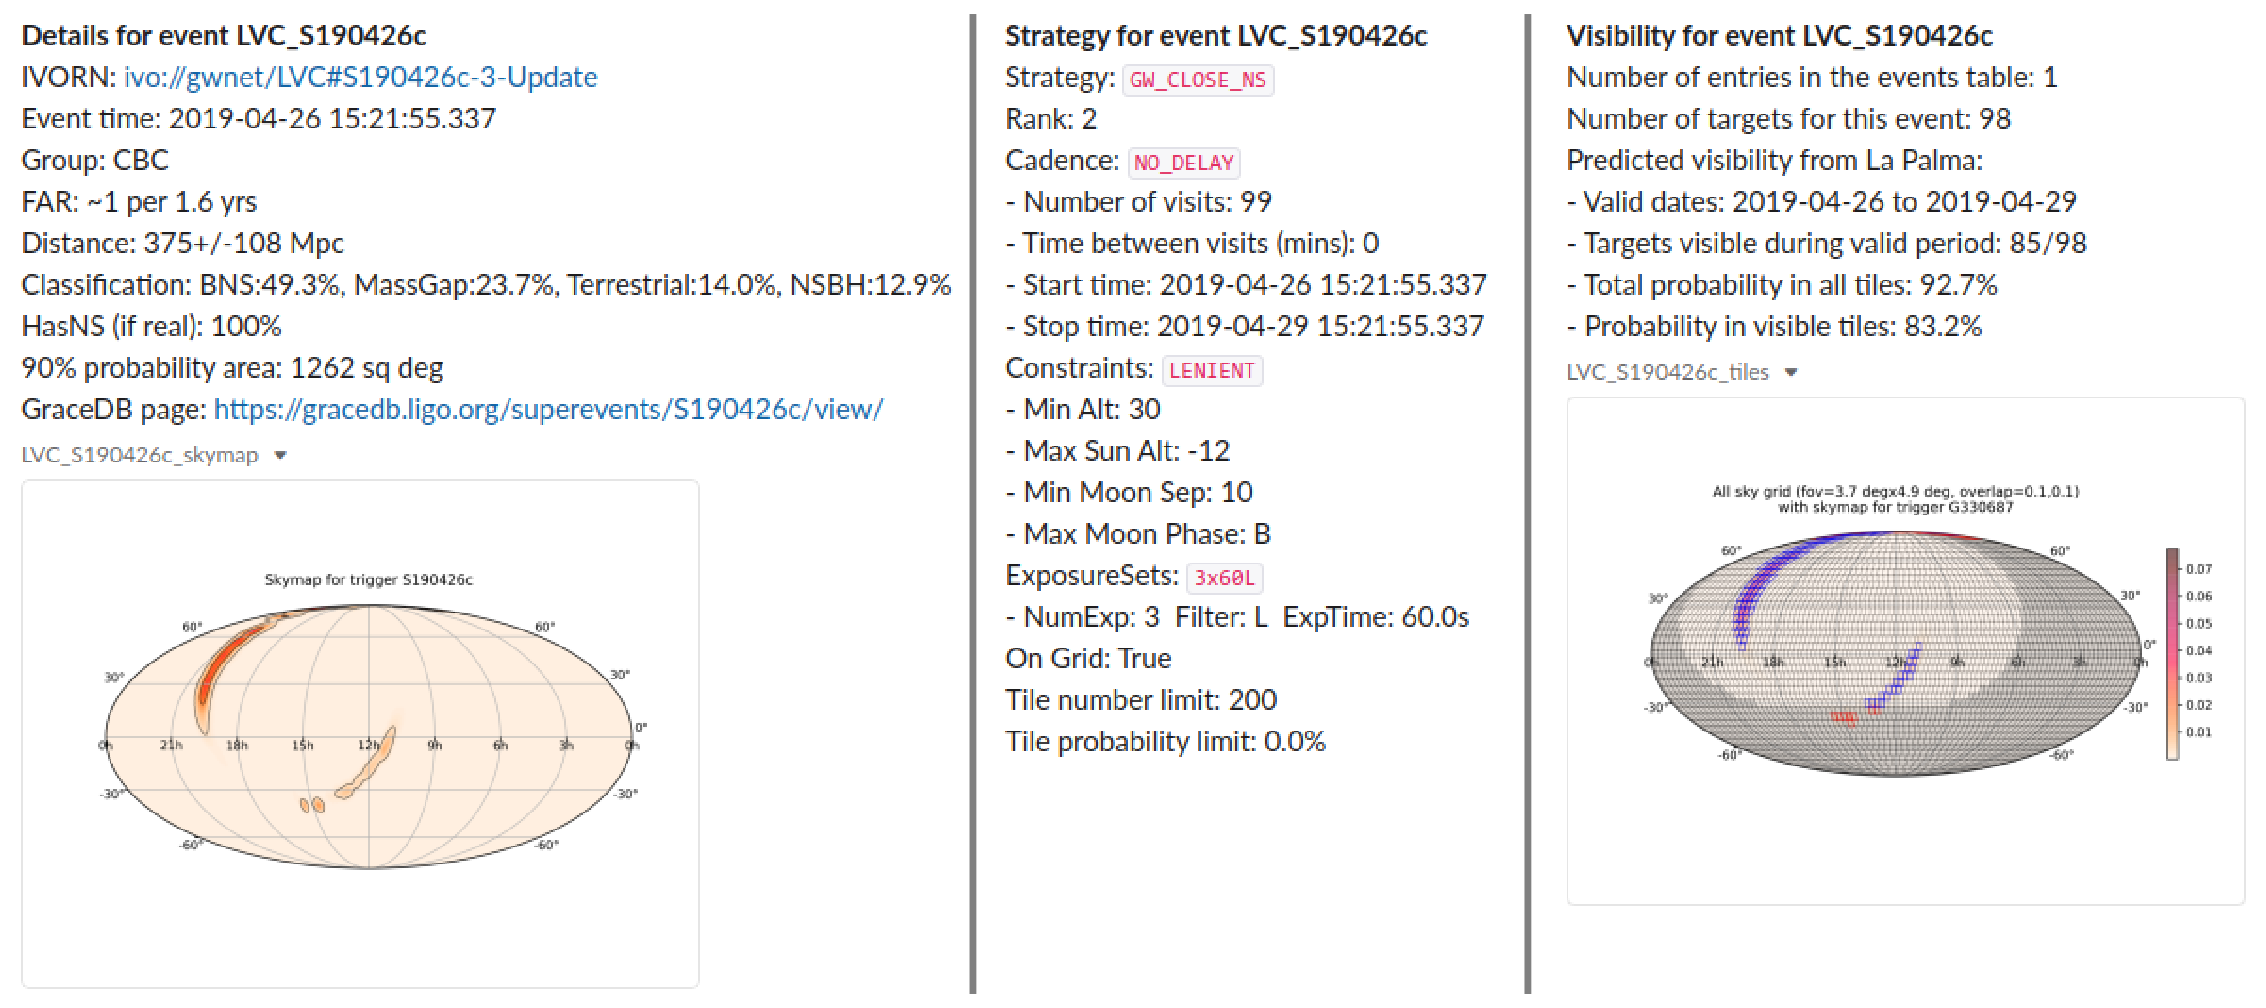
\includegraphics[width=\linewidth]{images/gototile_slack_side.png}
\end{center}
\caption[Slack alerts created by GOTO-tile for a GW event]{Slack alerts generated by the GOTO-tile event handler for a real gravitational wave event, S190426c.\\
\textbf{Left}: The first alert includes key information about the event gathered from the GCN notice, for \gls{gw} events that includes \gls{far}, classification and distance information, a link to the GraceDB entry and a skymap image generated by GOTO-tile.\\
\textbf{Centre}: The second alert details the event observing strategy (see \aref{sec:event_strategy}).\\
\textbf{Right}: The third alert gives the consequences of the applied strategy: the number of tiles inserted into the database and their visibility over the valid period. The attached GOTO-tile plot shows a prediction of which tiles covering the skymap will be visible.
}
\label{fig:gototile_slack}
\end{sidewaysfigure}

\end{colsection}

% ~~~~~~~~~~~~~~~~~~~~

\newpage

\subsection{Determining observation strategies}
\label{sec:event_strategy}
\begin{colsection}

An important function of the GOTO-alert event handler is to determine the specific strategy to be used to observe follow-up observations for each interesting event. The \gls{gtecs} observation database (see \aref{sec:obsdb}) contains a large number of tables and structures to enable tailoring observations to the properties of the triggering event, either by altering the validity, priority and cadence of the resulting pointings inserted into the scheduler queue (see \aref{sec:scheduler}) or by customising the commands issued by the pilot when that pointing is selected (see \aref{sec:pilot}).

The term \textit{strategy} is used deliberately to differentiate from the actions carried out by the on-site pilot, which might be better called \textit{tactics}. Properly defined, strategy defines long-term aims and objectives (consider generals directing a war far from the front lines, or the coach of a sports team) whereas tactics are the on-the-ground implementation details used to move towards those objectives (determined by the captain in the trenches or on the pitch). The sentinel decides the observing strategy for a particular event, using the structures and functions within GOTO-alert. These decisions are then communicated to the pilot through the observation database, which decides what to do independently using the scheduler and the local conditions. Only then are commands sent to the hardware daemons to put the plan into action: like the soldiers on the battlefield or players on the pitch theirs is not to reason why but to carry out their orders as issued.

The importance of defining such a distinction is that the strategies and objectives decided by the sentinel can only ever be aspirational, for the best-case scenario. A detailed plan of follow-up observations for a transient event can be determined, but if the target is not visible from La Palma, or it is currently raining, then the pilot will clearly not be able to implement those plans. The sentinel is designed to be aspirational and not consider smaller details such as these in order to make it independent of physical hardware. Ultimately GOTO is envisioned to occupy multiple sites across the world, as described in \aref{sec:goto_expansion}, but the intention is that they will all still be taking orders from a single central sentinel and database (see \aref{sec:gtecs_multisite}).

\newpage

\begin{figure}[t]
\begin{center}

\includegraphics[width=\linewidth]{images/strategy_flowchart.pdf}
\end{center}
\caption[Decision tree for determining event strategy]{Decision tree for determining event strategy.
}
\label{fig:strategy_flowchart}
\end{figure}

In order to decide the observation strategy for a given event the GOTO-alert event handler uses the decision tree shown in \aref{fig:strategy_flowchart}. The codes at the end of the branches (\code{GW\_CLOSE\_NS}, \code{GRB\_FERMI} etc) are the individual strategies, and they correspond to keys in the strategy dictionary defined within GOTO-alert as shown in \aref{tab:strategy_dict}. Each strategy corresponds to an integer rank as well as further keys relating to cadence, constraints and exposure sets which are keys in three additional dictionaries shown in \aref{tab:cadence_dict}, \aref{tab:constraints_dict} and \aref{tab:exposuresets_dict}. Through this structure all the values required for inserting an event into the database are defined, and it is also simple to modify these strategies or add in new ones.

\clearpage

% -----

\begin{table}[!p]
\begin{center}
\begin{tabular}{lclll}

Strategy             & Rank & Cadence                        & Constraints    & ExposureSets \\
\midrule
\code{GW\_CLOSE\_NS} &    2 & \code{NO\_DELAY}               & \code{LENIENT} & \code{3x60L} \\ % chktex 29
\code{GW\_FAR\_NS}   &   13 & \code{NO\_DELAY}               & \code{LENIENT} & \code{3x60L} \\ % chktex 29
\code{GW\_CLOSE\_BH} &   24 & \code{TWO\_NIGHTS}             & \code{LENIENT} & \code{3x60L} \\ % chktex 29
\code{GW\_FAR\_BH}   &  105 & \code{TWO\_NIGHTS}             & \code{LENIENT} & \code{3x60L} \\ % chktex 29
\code{GW\_BURST}     &   52 & \code{NO\_DELAY}               & \code{LENIENT} & \code{3x60L} \\ % chktex 29
\code{GRB\_SWIFT}    &  207 & \code{TWO\_FIRST\_ONE\_SECOND} & \code{NORMAL}  & \code{3x60L} \\ % chktex 29
\code{GRB\_FERMI}    &  218 & \code{TWO\_FIRST\_ONE\_SECOND} & \code{NORMAL}  & \code{3x60L} \\ % chktex 29

\end{tabular}
\end{center}
\caption[Event strategy dictionary keys]{Event strategy dictionary keys.}
\label{tab:strategy_dict}
\end{table}

% -----

\begin{table}[!p]
\begin{center}
\begin{tabular}{lccc}

Cadence                        & Number of visits & Hours between visits & Valid days \\
\midrule
\code{NO\_DELAY}               &               99 &                    0 &          3 \\
\code{TWO\_NIGHTS}             &                2 &                   12 &          3 \\
\code{TWO\_FIRST\_ONE\_SECOND} &                3 &                4, 12 &          3 \\

\end{tabular}
\end{center}
\caption[Cadence strategy dictionary keys]{Cadence strategy dictionary keys.}
\label{tab:cadence_dict}
\end{table}

% -----

\begin{table}[!p]
\begin{center}
\begin{tabular}{lcccl}

Constraints    & Min Alt          & Max Sun Alt       & Min Moon Separation & Max Moon Phase \\
\midrule
\code{LENIENT} & \SI{30}{\degree} & \SI{-15}{\degree} & \SI{30}{\degree}    &         Bright \\
\code{NORMAL}  & \SI{30}{\degree} & \SI{-12}{\degree} & \SI{30}{\degree}    &         Bright \\

\end{tabular}
\end{center}
\caption[Constraints strategy dictionary keys]{Constraints strategy dictionary keys.}
\label{tab:constraints_dict}
\end{table}

% -----

\begin{table}[!p]
\begin{center}
\begin{tabular}{lcccl}

ExposureSets   & Set position & Number of exposures &    Exposure time & Filter \\
\midrule
\code{3x60L}   &          1/1 &                   3 & \SI{60}{\second} &      \textit{L} \\ % chktex 29
\code{3x60RGB} &          1/3 &                   1 & \SI{60}{\second} &      \textit{R} \\ % chktex 29
               &          2/3 &                   1 & \SI{60}{\second} &      \textit{G} \\ % chktex 29
               &          3/3 &                   1 & \SI{60}{\second} &      \textit{B} \\ % chktex 29

\end{tabular}
\end{center}
\caption[ExposureSets strategy dictionary keys]{ExposureSets strategy dictionary keys.}
\label{tab:exposuresets_dict}
\end{table}

% -----

\clearpage

The strategies determined using \aref{fig:strategy_flowchart} and described in \aref{tab:strategy_dict}, \aref{tab:cadence_dict}, \aref{tab:constraints_dict} and \aref{tab:exposuresets_dict} are the ones used within the \gls{goto} sentinel at the time of writing. They were decided based on the priorities of the \gls{goto} project as described in the following pages.

The first distinction is between gravitational wave and gamma-ray burst events. \gls{goto}'s primary priority is searching for \gls{gw} counterparts, with any \gls{grb} follow-up being a useful but decidedly lower-priority use of \gls{goto}'s time. Therefore all \gls{gw} events have ranks considerably higher than \gls{grb} events, and due to their importance to the project \gls{gw} events also use more lenient constraints (defined in \aref{tab:constraints_dict}) than the normal ones used by \gls{grb} events and the all-sky survey.

The highest priority for \gls{goto} should always be \gls{gw} events that are predicted to contain a neutron star component, as they are the ones that are expected to produce an electromagnetic counterpart that \gls{goto} could detect (see the definitions of ``HasNS'' and ``HasRemnant'' in \aref{sec:event_handling}). This difference is expressed in the different cadence strategies used for each:

\begin{itemize}
    \item Neutron star events have no delay between visits, meaning once a pointing is completed it will be immediately re-inserted into the queue (with its rank increased by 10). So for these events once the telescope has observed all the visible tiles once it will immediately start covering the map again, and by default this will continue until it reaches the stop time three days after the event (or until it reaches 99 observations of each tile, which is inserted just as a maximum and isn't expected to be reached within three nights).
    \item Black hole events on the other hand have a more limited \code{TWO\_NIGHTS} strategy, which only requires two observations of each tile with at least 12 hours between them (which in practice means in two subsequent nights).
\end{itemize}

For both neutron star and black hole events a distinction is also made between ``close'' and ``far'' events based on their reported source distance: a close neutron star event is defined to be within \SI{400}{\mega\parsec} while a close binary black hole event is within \SI{100}{\mega\parsec}. The sole current detection of a gravitational wave counterpart, associated with GW170817, peaked in the optical at approximately 17th magnitude at a distance of \SI{40}{\mega\parsec} \citep{GW170817_followup}, corresponding to an absolute magnitude of -16. Using the equation for apparent magnitude

\begin{equation}
    m-M = -5 +5\log_{10}(d),
    \label{eq:magnitude}
\end{equation}

the GW170817 would have peaked above 19th magnitude out to a distance of \SI{100}{\mega\parsec} and above 22nd magnitude out to a distance of \SI{400}{\mega\parsec}. Binary-black hole mergers are not expected to produce the same amounts of ejected matter that would produce a kilonova, but some predictions suggest there may be material ejected from disks around one or more of the black holes which might reach 22nd magnitude if closer than \SI{100}{\mega\parsec} \citep{BBH_EM, BBH_Gompertz}. As a first approximation therefore the 22nd magnitude limits were adopted for the close/far distinction. Note this is a very arbitrary division, and not one particularly based on \gls{goto}'s capability (which is not able to detect sources down to 22nd magnitude). Instead it is a more a division into sources that \textit{could} have an optical counterpart visible from Earth.

The only difference in strategy between ``close'' and ``far'' events is that they are assigned different initial ranks when inserted into the database. The rest of the strategy including cadence and constraints are identical, and therefore the division is completely academic except in the case where multiple events exist in the observing queue at the same time. Should this happen then the ranking system provides a quick method to prioritise events for observations, assuming tiles for both events were visible at the same time. Using the ranks given in \aref{tab:strategy_dict} events from close neutron star mergers would be inserted at rank 2, while far mergers of the same type would be inserted at rank 13. As the rank of a pointing is increased by 10 every time it is observed this would prioritise two passes of the ``close'' skymap before the ``far'' skymap. The first observation would be at rank 2, the second at rank 12, and by the third it would be in the queue at rank 22. This however is lower than the initial rank of 13 for the ``far'' event, so that would then be higher in the queue. Any following observations would alternate between the two events: ``close'' pass 3 at rank 22, ``far'' pass 2 at rank 23, ``close'' pass 4 at rank 32 etc. The ranks for the other events are likewise carefully chosen: close \gls{bbh} events would be inserted at rank 24 and therefore fall behind the first three passes of a close NS or two passes of a far NS.\@ Far \gls{bbh} events are very unlikely to produce any visible optical counterparts, so although \gls{goto} will still consider them they are inserted at rank 105 well below several passes of any more promising \gls{gw} events.

What is currently not considered by the strategy definition is a \textit{maximum} valid distance, beyond which there is no point in \gls{goto} taking any action. \gls{lvc} detections have already reached out to the gigaparsec scale, and at those distances the chance of there being any optical counterpart visible from Earth is very low. At the time of writing \gls{gw} events are rare enough that there is little reason for \gls{goto} to follow up everything reported by the \gls{lvc}, in the future if necessary it would be easy to put a cap on what events \gls{goto} follows up based on distance or any other parameter (for example false-alarm rate).

Gravitational wave events from the LVC burst pipelines are hard to categorise as there is very little information to base any observation strategy on. As a compromise they use the same cadence strategy as neutron star events, but are inserted at rank 52 below any more promising events (aside from far \gls{bbh} events).

Gamma-ray burst events are also processed by the sentinel and inserted into the observation database. These are inserted at ranks above 200, ensuring that \gls{goto} will always prioritise gravitational wave follow up. \gls{grb} events use a different cadence strategy of \code{TWO\_FIRST\_ONE\_SECOND}, which as detailed in \aref{tab:cadence_dict} asks for three observations: two in the first night separated by 4 hours and another in the second night. This is a different test cadence recently implemented to attempt to account for the fast-fading nature of \gls{grb} afterglows, and is an example of more complex cadences allowed by the \gls{gtecs} scheduler. For gamma-ray burst events the only distinction is made between events originating from \textit{Swift} and \textit{Fermi}. Typically \textit{Swift}'s \gls{bat} detections are much better localised than those from \textit{Fermi}'s \gls{gbm}, and so in cases where a source is detected by both the \textit{Swift} detection should be prioritised. Further division could be made based on if the burst is classified by \textit{Fermi} as Long or Short, but this is not currently implemented.

Finally each strategy currently uses the same exposure sets as the all-sky survey: three sequential exposures using the \textit{L} filter lasting 60 seconds. A similar set of exposures using the coloured filters instead is shown in \aref{tab:exposuresets_dict} as a possible example of what could be defined, but is not currently used as part of any strategy.

It should be stressed that the strategies detailed in this sections are designed to just inform the default reaction of \gls{goto} to any incoming alert. It is not intended to be a perfect reaction in every case for the simple reason that there may well be later external input. For example the default strategy for a gravitational wave signal from a close neutron star source is to observe the tile inserted over and over until the three day limit has passed. In practice it should be clear after the first few passes if there is any counterpart candidate, in which case it is possible for a human to intervene and direct \gls{goto} to go take observations of particular tiles with promising candidates. Likewise after the first pass of a distant \gls{bbh} event no candidate is detected, and nothing has been reported from any other source, the decision could be made to not bother with the second pass the day after and just return to the all-sky survey. The strategies defined here are therefore designed to produce a reasonable default response from \gls{goto} but other human-guided are also an expected part of any follow-up campaign.

\end{colsection}

% ~~~~~~~~~~~~~~~~~~~~

\subsection{Inserting events into the observation database}
\label{sec:db_insert}
\begin{colsection}

Once the strategy has been defined then the sentinel needs to insert events into the observation database so they are visible to the scheduler (see Section \aref{sec:obsdb} and \aref{sec:scheduler}).

% ---------
\subsubsection{Previous records}

The first task is to check for existing records for this event in the observation database \code{Events} table. This is to account for updating events as revised VOEvent alerts are received, or in order to process retraction events. \gls{lvc} events have several stages: first a ``Preliminary'' alert is released as soon as the signal is detected, then an ``Initial'' alert is issued when it has been human-vetted. From then future versions are marked as ``Update'' alert, unless the event itself is found to be non-physical or below certain thresholds in which case a ``Retraction'' alert is issued. At any of these stages the event skymap might be modified shifting the observing area, and \gls{goto} needs to update to these changes. Therefore if a previous entry for a new event is detected then all of the old pointings that are still pending in the queue are deleted before the new ones are added. Should the event be of type \code{GWRetractionEvent} then this is where the function exits, as once the previous pointings are deleted then there are no more to replace them.

% ---------
\subsubsection{Mapping onto the all-sky grid}

Once previous event have been dealt with then the new entries in the database need to be created. All \gls{goto} pointings from the sentinel are defined \textit{on-grid}, meaning that they need to be mapped to the current GOTO-tile sky grid (see \aref{sec:grids}). The database \code{Grids} table contains the field of view and overlap parameters of the current grid as well as the algorithm used (see \aref{sec:algorithms}), allowing it to be reconstructed using GOTO-tile within the event handler. Once a GOTO-tile \code{SkyGrid} class has been created then a corresponding \code{SkyMap} class is made based on the information in the event. If it was created from a gravitational wave alert then it should have a URL to download the \gls{lvc}-created skymap. If instead it just has a coordinate and error radius, i.e.\ a \gls{grb} alert, then a new Gaussian skymap is constructed as described in \aref{sec:gaussian_skymaps}. Once both grid and map are ready then the skymap is mapped onto the grid simply using the class method \code{SkyGrid.apply\_skymap(SkyMap)}, which returns a table of tiles and associated contained probabilities (calculated as described in \aref{sec:mapping_skymaps}). %chktex 36

% ---------
\subsubsection{Selecting tiles}

The tile probability table created by GOTO-tile contains entries for every one of the thousands of tiles within the all-sky grid, of which a vast majority will contain a very small amount of the overall probability for any reasonably-well located skymap. Adding an entry to the database for every tile would therefore be unnecessary, and even harmful as the scheduling system is designed to complete a full pass of the visible tiles before going on to re-observe those already completed. On the other hand it's still important to add in enough tiles covering enough of the probability area to maximise the chance of detecting the source. Therefore there is a balance required between adding too many or too few tiles into the database.

There are multiple ways to chose which tiles to select. Initially GOTO-alert used a simple cut-off in terms of each tile's contained probability, chose each tile that contains greater than (for example)$1\%$ of the total probability. This hard limit however quickly proved to be unsuitable: spread-out skymaps might have few if any tiles which reach the limit, while for well-localised events adding tiles down to the $1\%$ level is redundant and would waste time observing them compared to revisiting higher probability tiles.

A different option was to keep the hard cut-off in terms of contained probability, but modify the limit for each skymap. One way of calculating thi was making the cut-off a function of the highest tile probability. For example a well-localised event might result in the highest-probability tile containing $30\%$ of the probability, so with a 10\% cut-off all tiles containing 3\% or above would be added. On the other hand a spread-out skymap might have a highest tile only containing 2\%, so then all tiles with 0.2\% or above would be added. Other possible values to base this off were the on-sky areas of the 90\% or 50\% contours. Ultimately all the methods that used a hard contained probability cut-off proved to be not very responsive to the geographic spread of the skymap, and determining the precise proportionality constant (e.g. 10\% in the above example) was hard to balance between large and small maps.

Another alternative method was to start with the highest probability tile and then add on subsequent tiles until the total probability covered reaches some target value, e.g. 90\% of the skymap. This method was originally used by GOTO-tile, but is relatively complicated to calculate when considering grids with overlap between the tiles. Just selecting tiles based on their contained probability will over-count overlapping regions, and so the final selected tiles which nominally contain 90\% of the probability will actually contain less. The solution to this is to re-generate the skymap after selecting each tile with the already-selected pixels set to 0, but this then becomes a non-trivial optimisation problem that is computationally intensive for limited gain compared to other possibilities.

The ultimately preferred alternative is to instead select tiles based on their position in the sky contours. As discussed in \aref{sec:mapping_skymaps} finding which contour each tile falls within is not easy to calculate. You could, for example, say a tile is only within a given contour area if \textit{every} pixel contained within the tile is within that contour. However \gls{goto}'s large tile areas are often wider than the long, stretched out probability areas typical of \gls{lvc} skymaps, so few if any tiles would meet this strict criteria. The mirror to this is to say a tile is within a contour if \textit{any} of its contained pixels are within the contour, which is the same as using the minimum of the contained contour values. This will find every tile covering the contour area even if only the smallest fraction of the tile's area is within that region, which leads to over-selecting tiles. The balanced alternative is to find the \textit{mean} contour value within the tile, which is the chosen method used within GOTO-alert: selecting all tiles which have a mean contour value within 90\%.

Four different algorithms applied to real \gls{lvc} skymaps are shown below in Figure \aref{fig:tiling_S190521r}, \aref{fig:tiling_GW170817} and \aref{fig:tiling_S190425z}. The upper plot in each shows the probability skymap as received from the \gls{lvc}. The green and red tile selections in the centre-left and centre-right plots show selecting all tiles based on their minimum contour value, with at least some portion located within the 50\% and 90\% contour areas respectively. The lower-left plot shows tiles containing more than 1\% of the total probability in blue, and the lower-right plot shows the compromise solution of the tiles with a mean pixel contour value of 90\% or less in yellow.

% -----

\begin{figure}[p]
\begin{center}
\begin{tabular}{cc}
\multicolumn{2}{c}{Prefered probability skymap for superevent S190521r:}
\\
\multicolumn{2}{c}{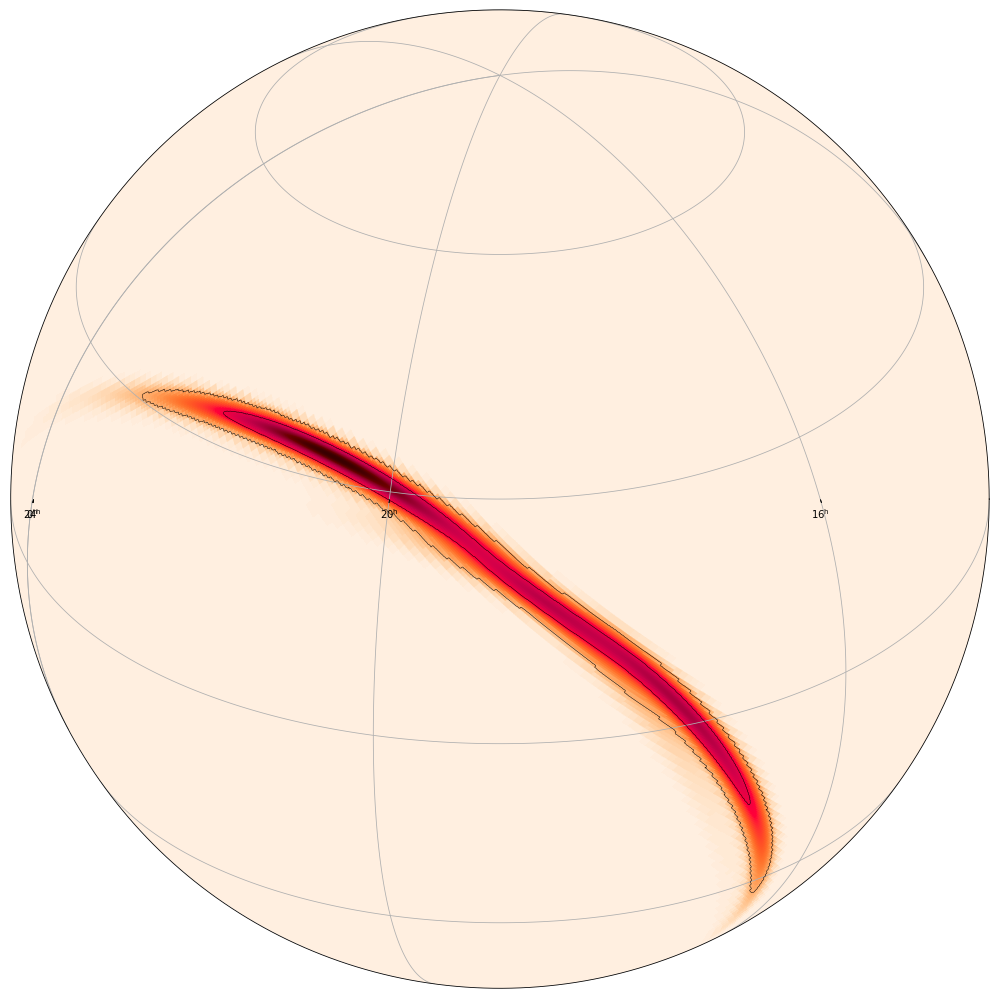
\includegraphics[width=0.5\linewidth]{images/tiling/1_0.png}}
\\
Tiles within 50\% contour: &
Tiles within 90\% contour:
\\
47 tiles, covering 86\% &
86 tiles, covering 98\%
\\
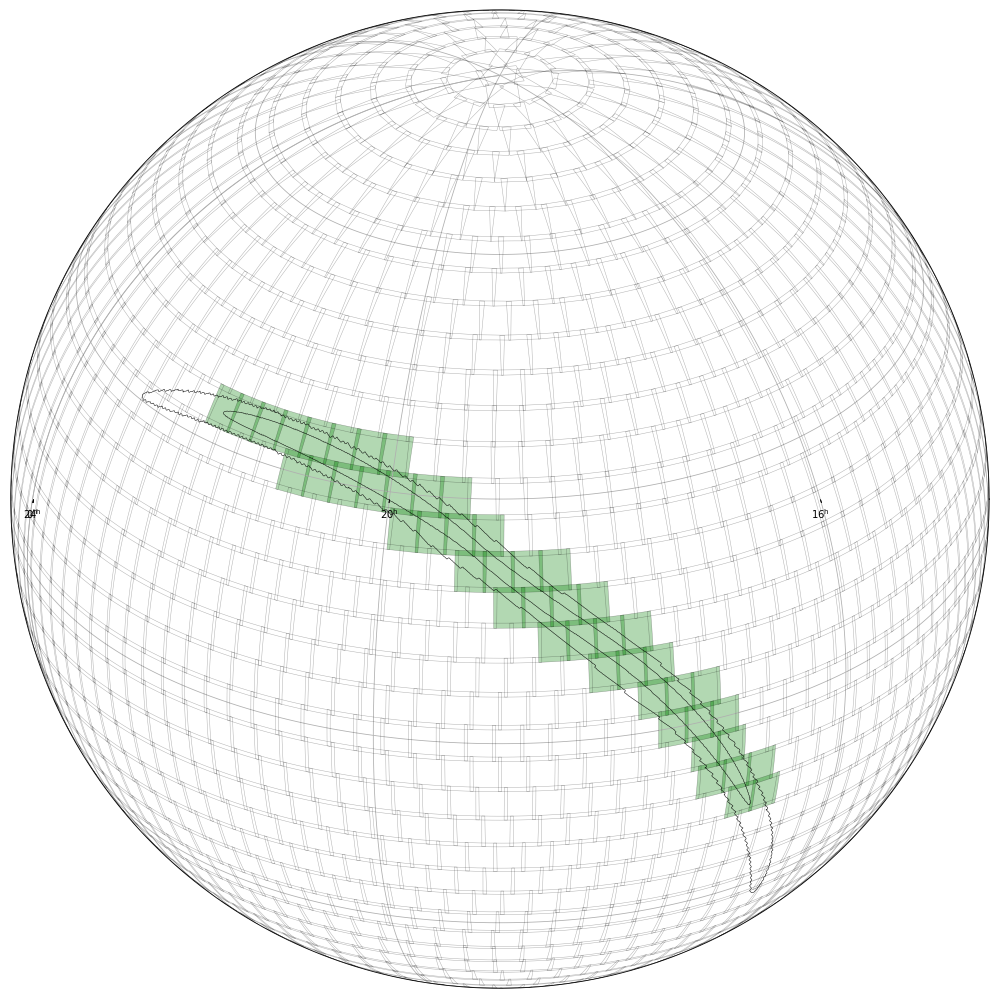
\includegraphics[width=0.25\linewidth]{images/tiling/1_c.png} &
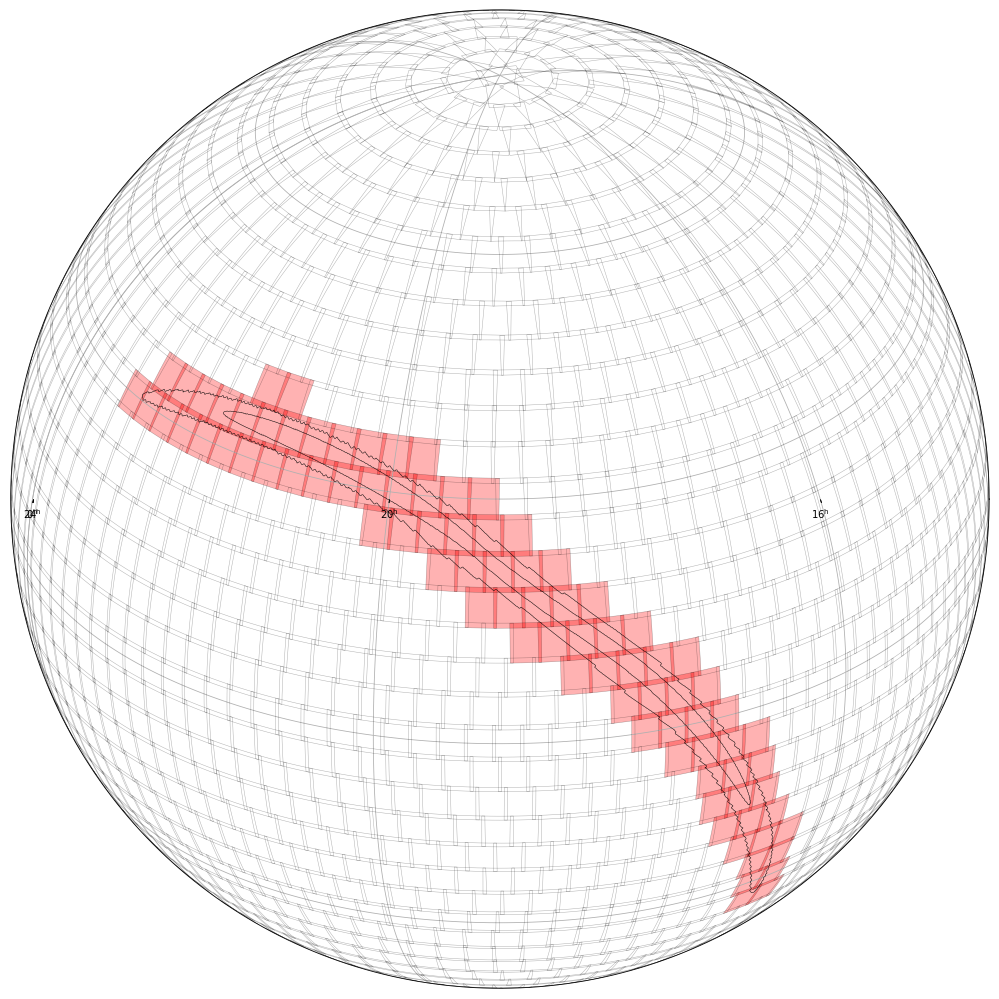
\includegraphics[width=0.25\linewidth]{images/tiling/1_d.png}
\\
Tiles with probability > 1\%: &
Tiles with mean contour within 90\%:
\\
41 tiles, covering 90\% &
42 tiles, covering 91\%
\\
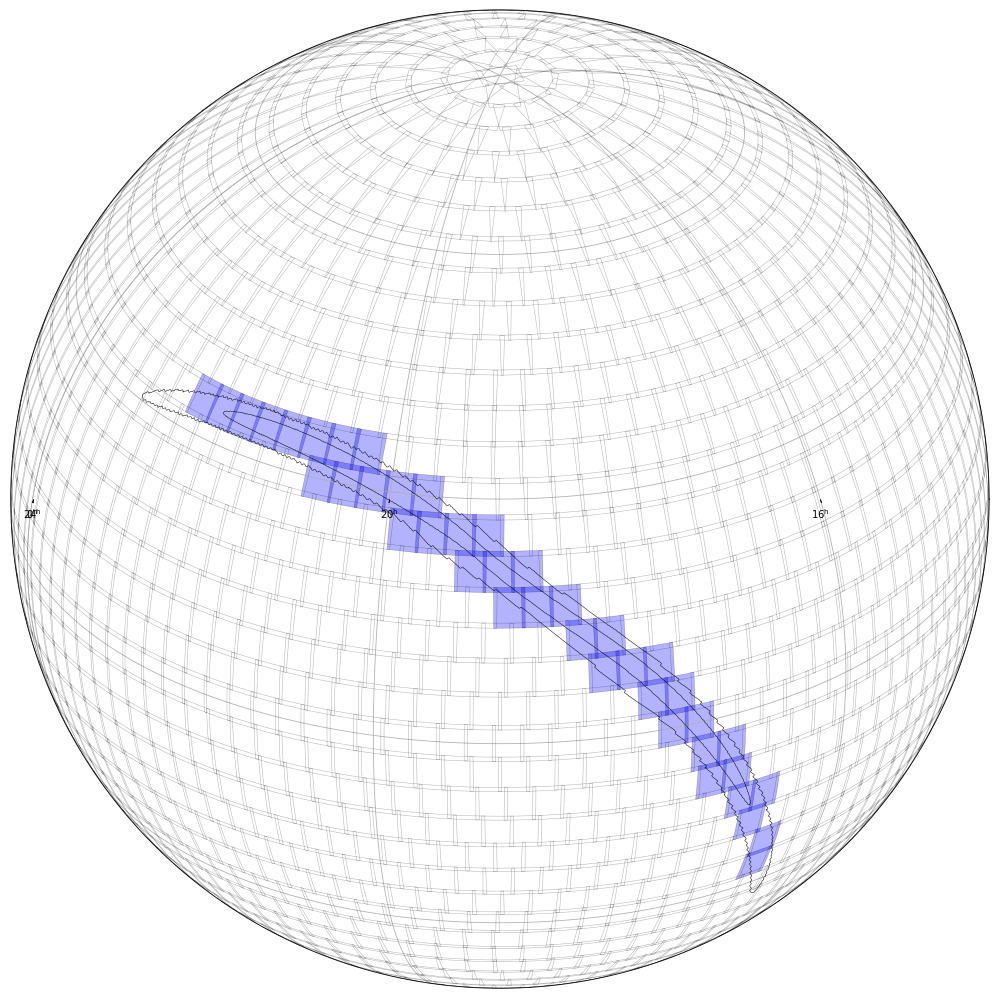
\includegraphics[width=0.25\linewidth]{images/tiling/1_a.png} &
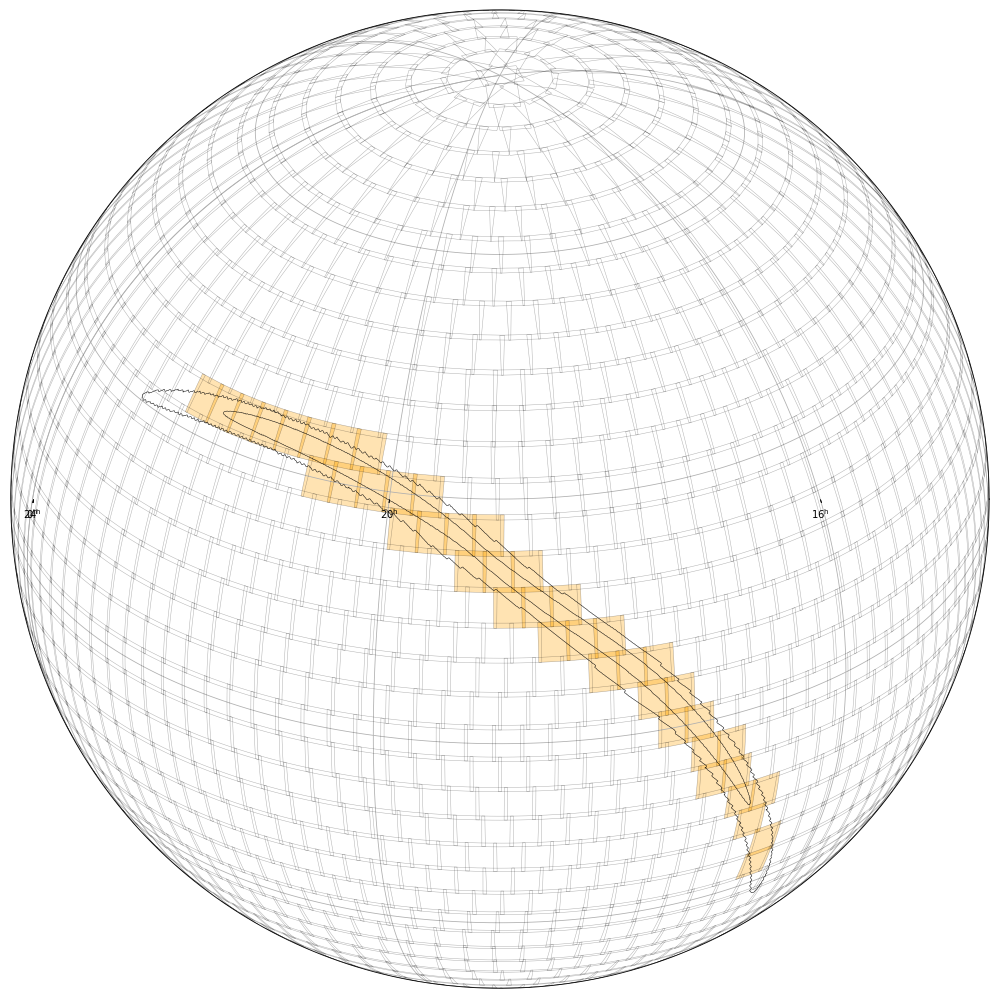
\includegraphics[width=0.25\linewidth]{images/tiling/1_b.png}
\\

\end{tabular}
\end{center}
\caption[Different tile selection methods for S190521r]{Different tile selection methods applied to the skymap for \gls{lvc} event S190521r.\\
This is a very typical \gls{gw} skymap, and one for which the basic method of choosing tiles with a contained probability of greater than 1\% (lower-left, in blue) works well and produces almost the same set of tiles as the improved mean contour method (lower-right, in yellow). Note the inefficiencies of covering the full contours, the 50\% contour (centre-left, in green) covers less probability with more tiles than either of the lower two methods.
}
\label{fig:tiling_S190521r}
\end{figure}

% -----

\begin{figure}[p]
\begin{center}
\begin{tabular}{cc}
\multicolumn{2}{c}{Final probability skymap for event GW170817:}
\\
\multicolumn{2}{c}{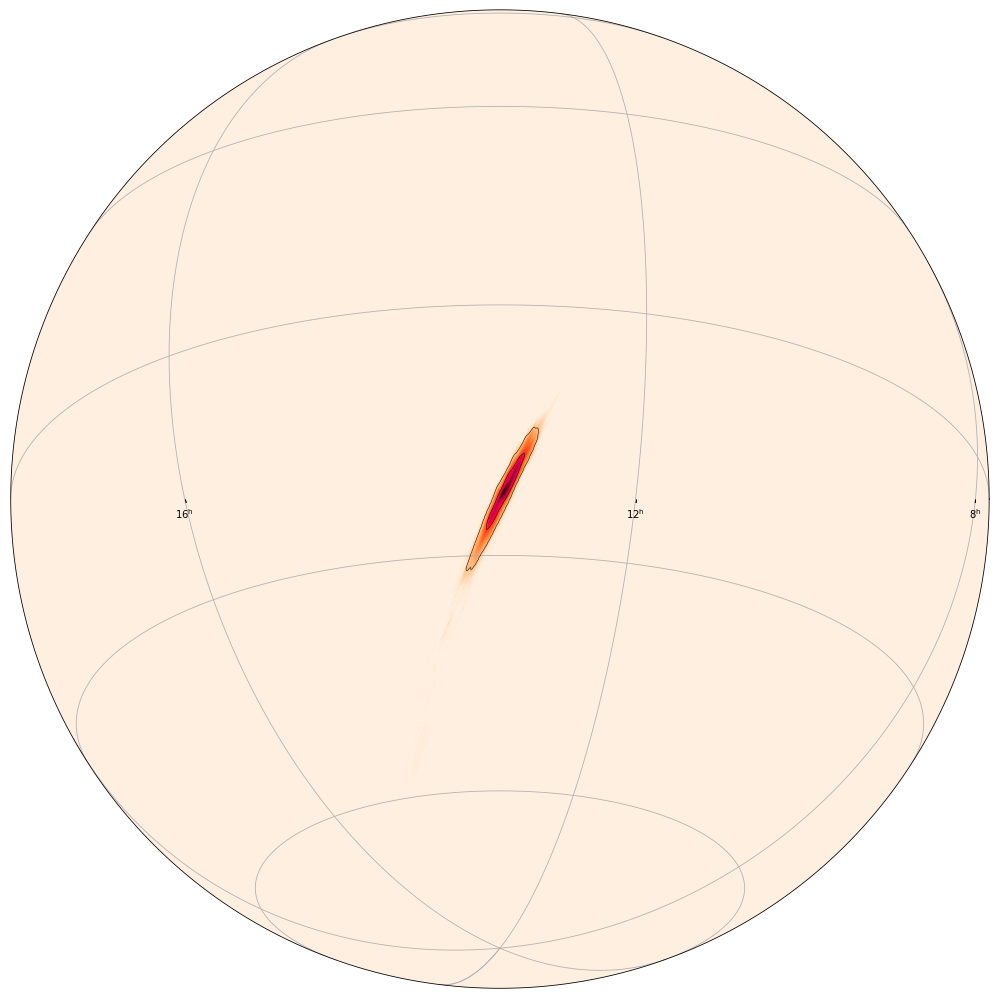
\includegraphics[width=0.5\linewidth]{images/tiling/2_0.png}}
\\
Tiles within 50\% contour: &
Tiles within 90\% contour:
\\
6 tiles, covering 88\% &
11 tiles, covering 96\%
\\
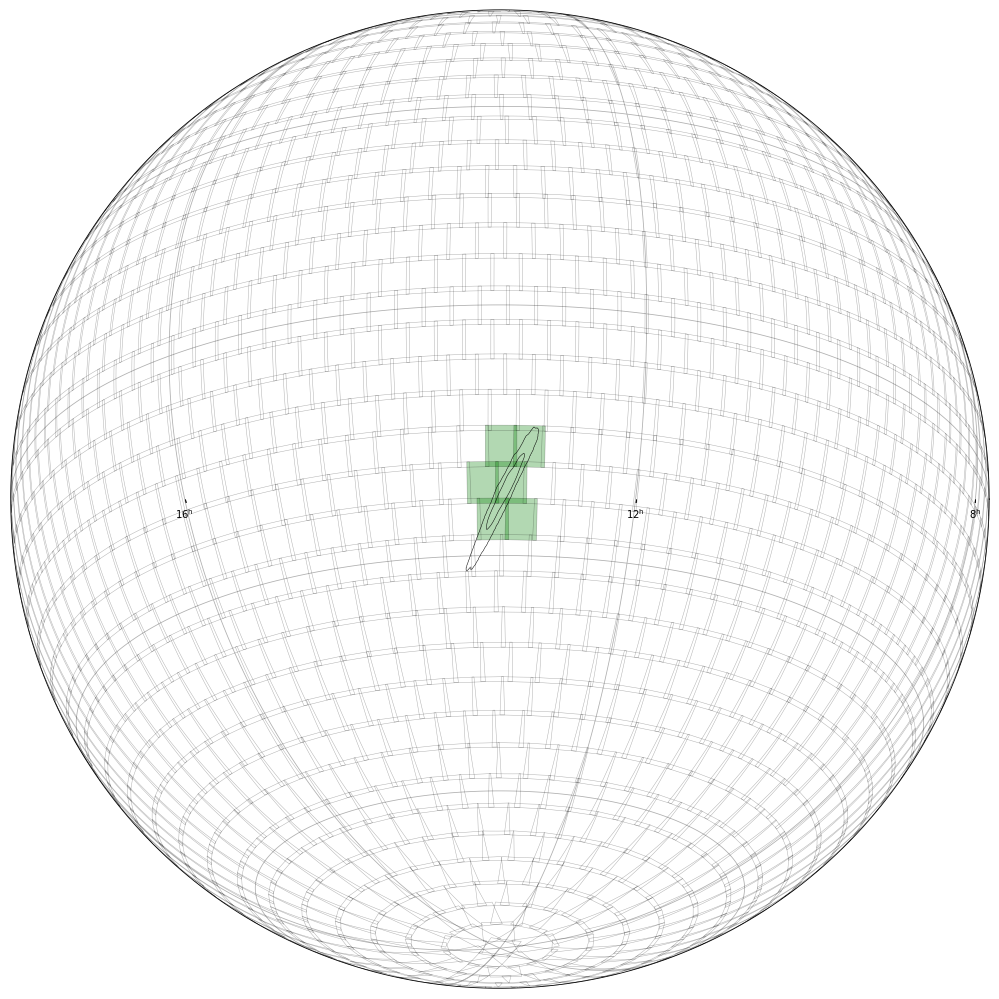
\includegraphics[width=0.25\linewidth]{images/tiling/2_c.png} &
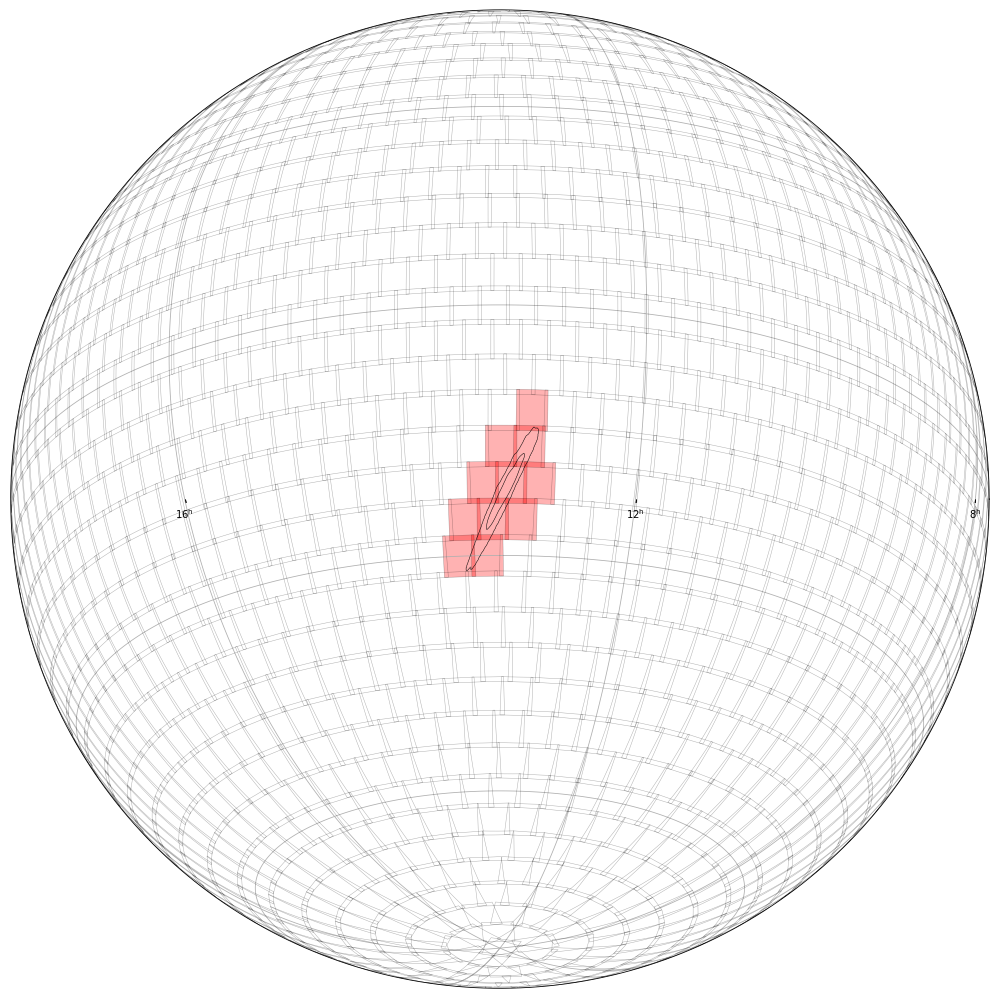
\includegraphics[width=0.25\linewidth]{images/tiling/2_d.png}
\\
Tiles with probability > 1\%: &
Tiles with mean contour within 90\%:
\\
10 tiles, covering 98\% &
3 tiles, covering 88\%
\\
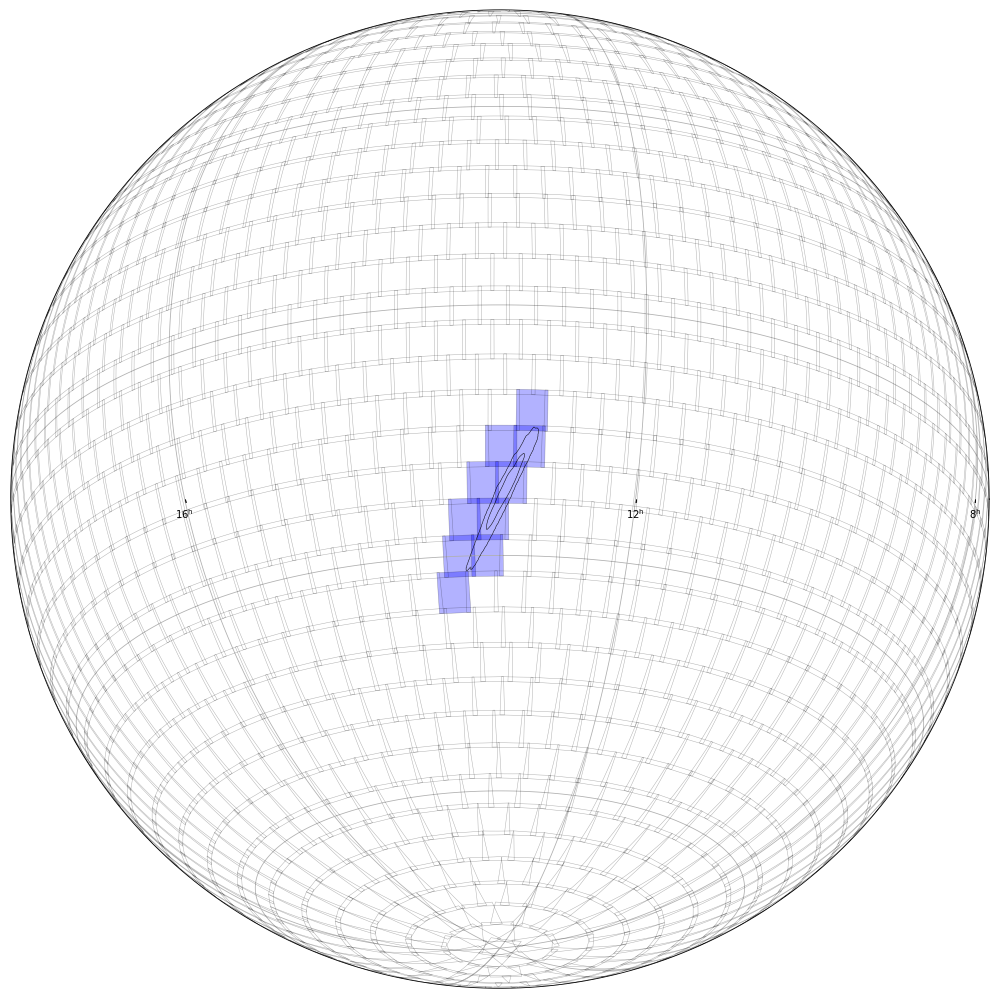
\includegraphics[width=0.25\linewidth]{images/tiling/2_a.png} &
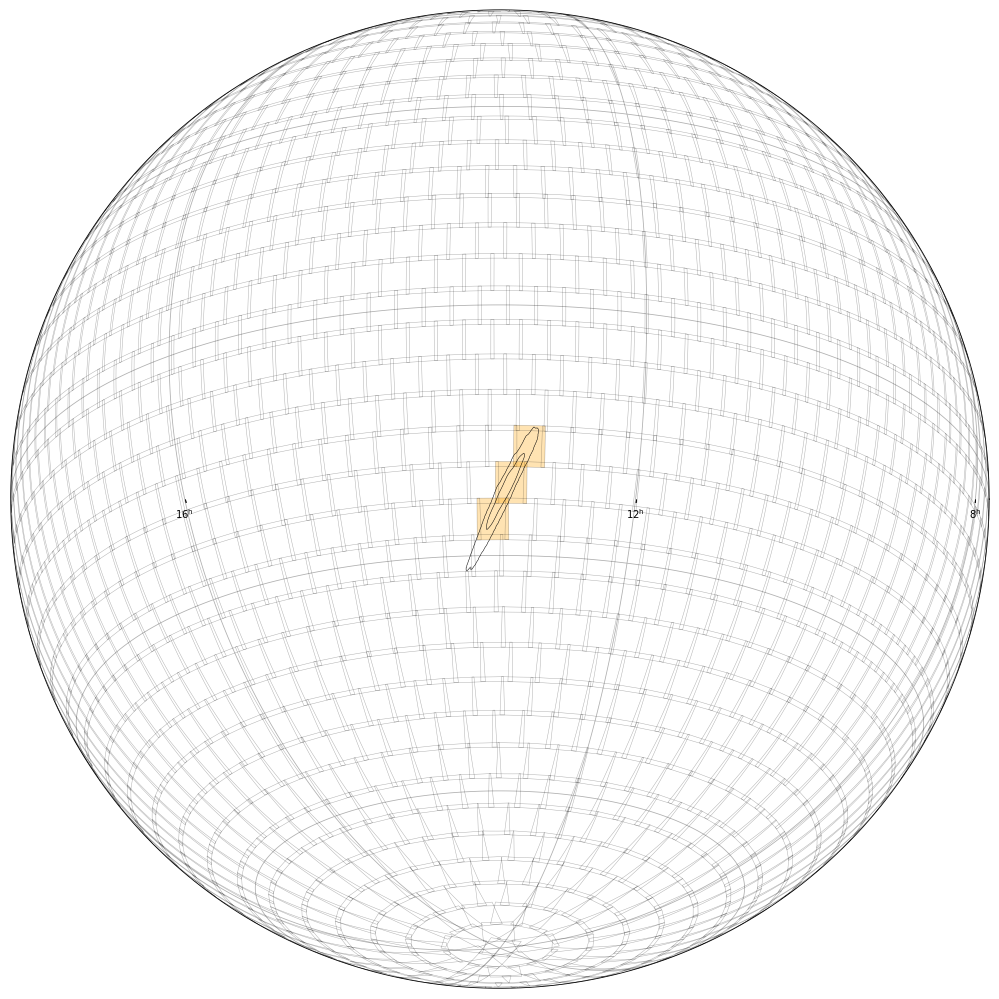
\includegraphics[width=0.25\linewidth]{images/tiling/2_b.png}
\\

\end{tabular}
\end{center}
\caption[Different tile selection methods for GW170817]{Different tile selection methods applied to the skymap for \gls{lvc} event GW170817.\\
This skymap is atypically well localised. In this case the simple 1\% limit (lower-left, in blue) selects a large number of redundant tiles. The inefficiencies of the contour methods are also visible, the 50\% selection limit (centre-left, in green) covers the same total probability as the mean contour method (lower-right, in yellow) but with twice the number of tiles. Note the location of the actual counterpart (as shown in \aref{fig:170817_gw}) was selected by all of these methods.
}
\label{fig:tiling_GW170817}
\end{figure}

% -----

\begin{figure}[p]
\begin{center}
\begin{tabular}{cc}
\multicolumn{2}{c}{Prefered probability skymap for superevent S190425z:}
\\
\multicolumn{2}{c}{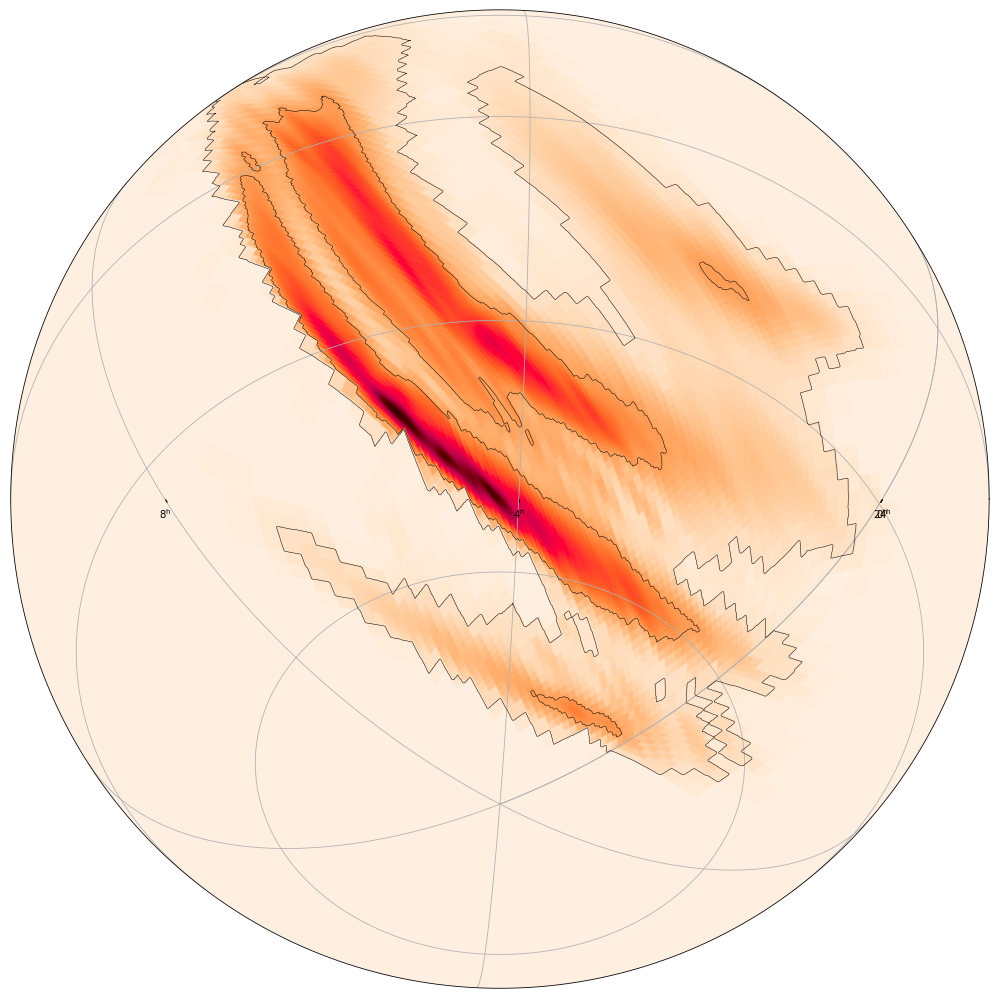
\includegraphics[width=0.5\linewidth]{images/tiling/3_0.png}}
\\
Tiles within 50\% contour: &
Tiles within 90\% contour:
\\
207 tiles, covering 67\% &
753 tiles, covering 95\%
\\
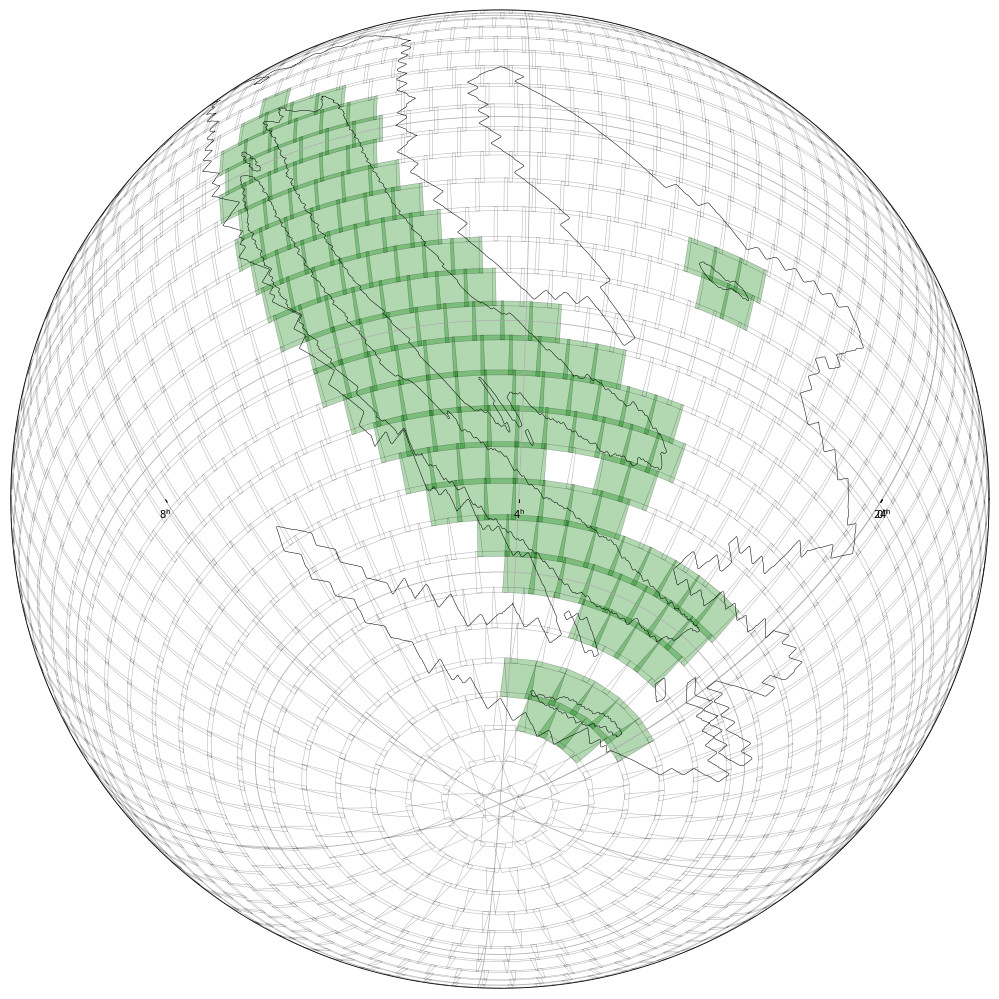
\includegraphics[width=0.25\linewidth]{images/tiling/3_c.png} &
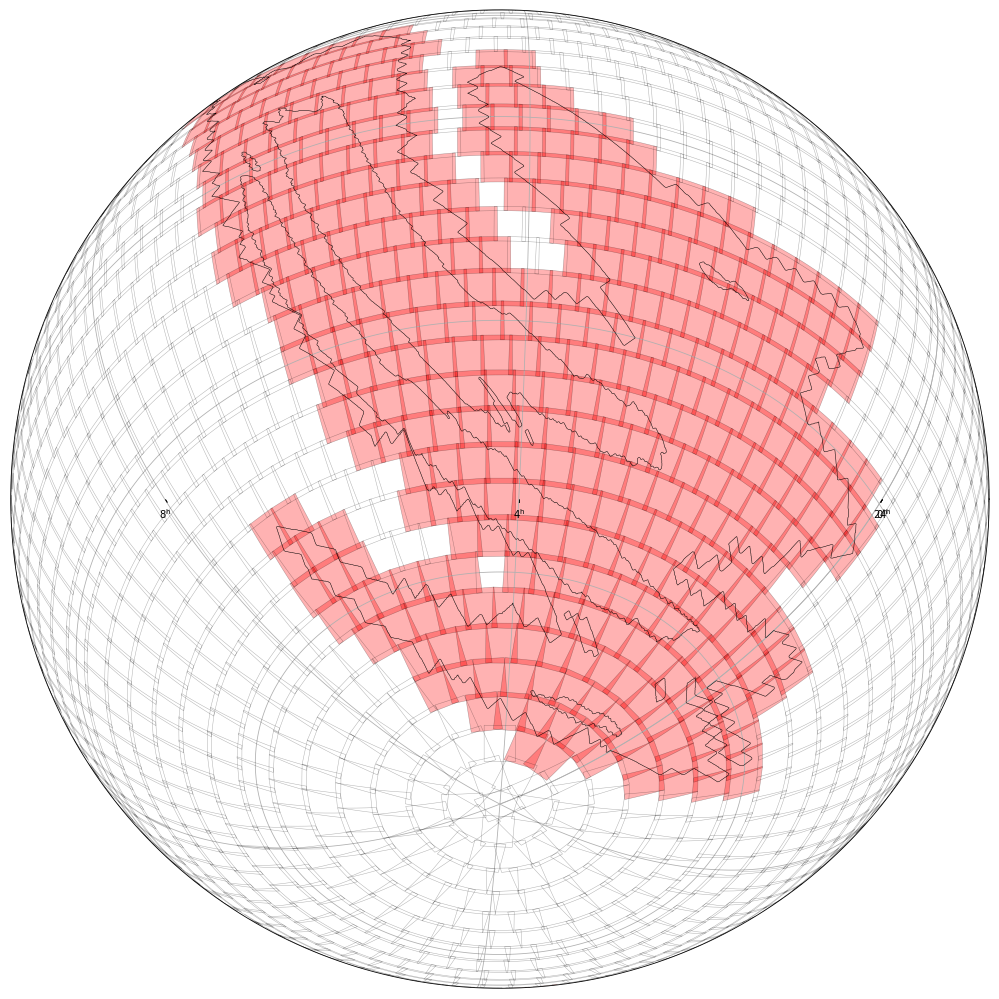
\includegraphics[width=0.25\linewidth]{images/tiling/3_d.png}
\\
Tiles with probability > 1\%: &
Tiles with mean contour within 90\%:
\\
10 tiles, covering 11\% &
548 tiles, covering 91\%
\\
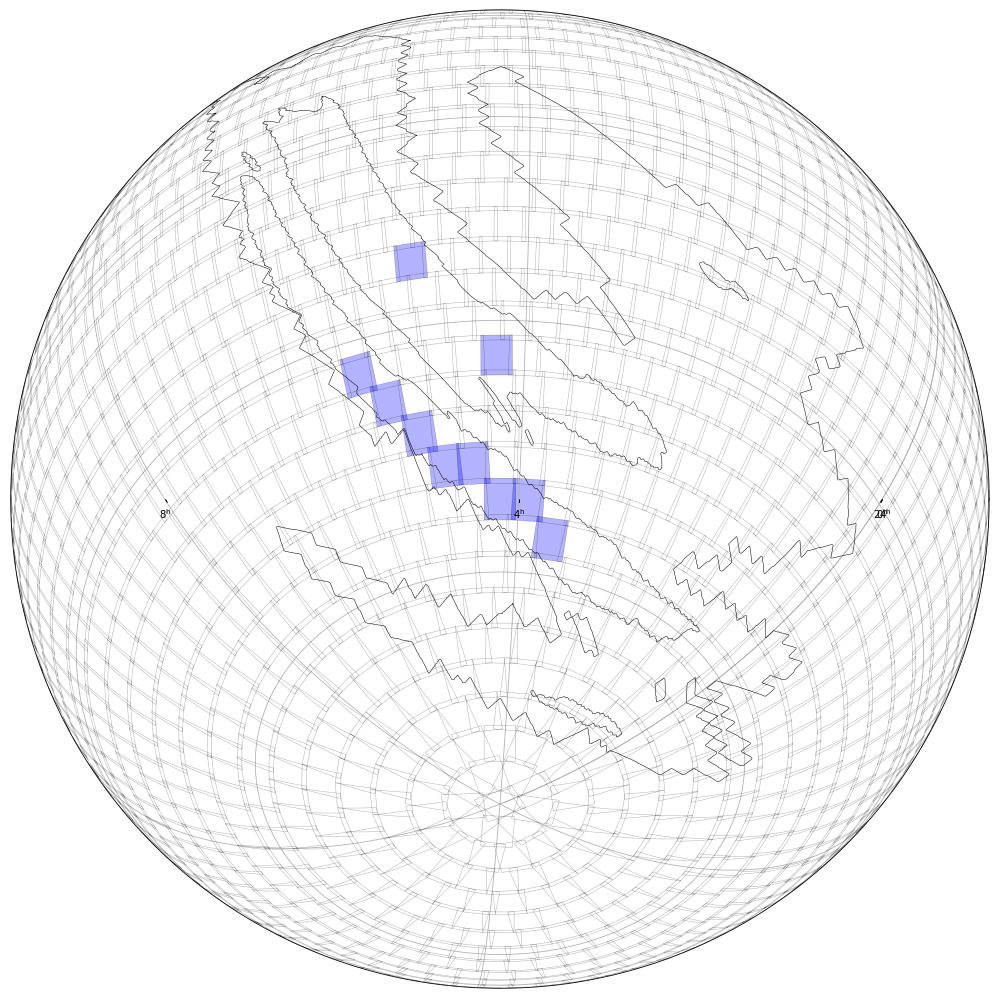
\includegraphics[width=0.25\linewidth]{images/tiling/3_a.png} &
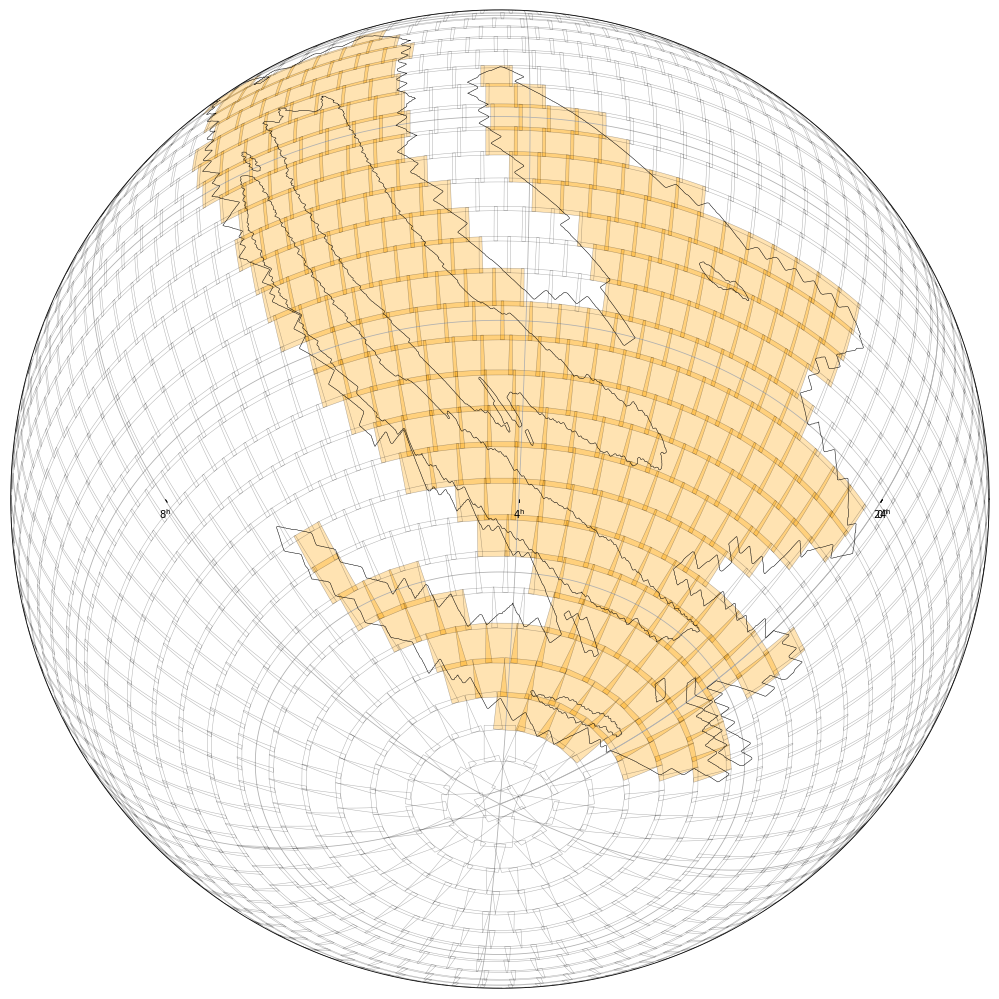
\includegraphics[width=0.25\linewidth]{images/tiling/3_b.png}
\\

\end{tabular}
\end{center}
\caption[Different tile selection methods for S190425z]{Different tile selection methods applied to the skymap for \gls{lvc} event S190425z.\\
This is an atypically large skymap. The fixed 1\% limit (lower-left, in blue) is clearly unsuitable to be used in this case. The mean contour method (lower-right, in yellow) is a reasonable compromise between the two centre contour methods, covering just 4\% less than the full 90\% contour selection but with 205 fewer tiles. Note 548 tiles would still be too many to easily observe for the 4-UT system, so they would be limited to the top 200 sorted by probability.
}
\label{fig:tiling_S190425z}
\end{figure}

% -----

\clearpage

Once the chosen tiles have been selected then entries can be inserted into the observing database (defined in \aref{sec:obsdb}). First a new entry in the \code{events} table is added for this event, containing the source, type, ID and \gls{ivorn}. Then an entry in the \code{surveys} table is also created in order to group together all the pointings from this particular event. Although it is currently not used, the database is defined to allow multiple surveys per event. For example, there could be a quick initial survey in a wide-passband filter that prioritises possible host galaxies followed by a slower survey using the colour filters and longer exposure times that focuses on covering the skymap. But at the time of writing each event only has a single survey defined.

Finally the individual tiles are inserted as entries in the \code{mpointings} table. Each is connected to an entry in the \code{grid\_tiles} table for this particular grid, and the tile probabilities are stored as corresponding entries in the \code{survey\_tiles} table. The most important entries for the mpointings are the rank, target constraint values (minimum altitude, moon phase etc), the time block parameters (the time between pointings being valid) and the actual exposure settings (exposure time, filter, number in a set). These are found from the event strategy as described in \aref{sec:event_strategy}. Once the mpointings are defined the first pointings are also created and added to the database \code{pointings} table, to insure they become immediately valid in the queue without having to wait for the caretaker to create them.

After all of these entries are added to the database then the event has been successfully handled. When the scheduler next fetches the queue the pointings should be there ready to observe, and if they are valid the highest priority will be sent to the pilot to begin follow-up observations.

\end{colsection}

% ~~~~~~~~~~~~~~~~~~~~

\end{colsection}

% ########################################
